% !TEX program = xelatex
\documentclass[11pt,a4paper,fontset=fandol]{ctexart}

\newcommand{\coursecode}{SC4061}
\newcommand{\coursetitle}{AI for Computer Vision}
\newcommand{\academicyear}{AY2026--27 Semester 1}
\usepackage[margin=25mm]{geometry}
\usepackage{amsmath,amssymb,amsthm,bm,mathtools}
\usepackage{booktabs,tabularx}
\usepackage{enumitem}
\usepackage{graphicx}
\usepackage{xcolor}
\usepackage{tikz}
\usepackage{fancyhdr}
\usepackage{hyperref}
\usepackage[nameinlink,noabbrev]{cleveref}
\usetikzlibrary{arrows.meta,calc,fit,positioning}

\definecolor{ntuRed}{HTML}{D71440}
\definecolor{noteBlue}{HTML}{1F4E79}
\definecolor{verifyOrange}{HTML}{A64B00}

\hypersetup{
  colorlinks=true,
  linkcolor=noteBlue,
  citecolor=noteBlue,
  urlcolor=noteBlue,
  pdftitle={\coursecode: \coursetitle},
  pdfsubject={\academicyear\ 课程学习笔记}
}

\setlength{\parindent}{0pt}
\setlength{\parskip}{0.6em}
\setlist{itemsep=0.25em,topsep=0.35em}
\graphicspath{{figures/}}

\pagestyle{fancy}
\fancyhf{}
\lhead{\coursecode}
\rhead{\coursetitle}
\cfoot{\thepage}
\setlength{\headheight}{14pt}

\newtheorem{definition}{Definition（定义）}[section]
\newtheorem{theorem}[definition]{Theorem（定理）}
\newtheorem{proposition}[definition]{Proposition（命题）}
\newtheorem{example}[definition]{Example（例）}
\newtheorem{remark}[definition]{Remark（说明）}

\newcommand{\recordid}[1]{%
  \textcolor{noteBlue}{\textbf{编号：} \texttt{#1}}%
}

\newcommand{\lecturemeta}[6]{%
  \begin{center}
    \begin{tabularx}{\textwidth}{@{}lX@{}}
      \toprule
      课堂编号 & \texttt{#1} \\
      上课日期 & #2 \\
      主要资料 & #3 \\
      覆盖范围 & #4 \\
      视频补充 & #5 \\
      人工确认 & #6 \\
      \bottomrule
    \end{tabularx}
  \end{center}
}

\newcommand{\exercisemeta}[5]{%
  \begin{center}
    \begin{tabularx}{\textwidth}{@{}lX@{}}
      \toprule
      题组编号 & \texttt{#1} \\
      对应日期 & #2 \\
      主要来源 & #3 \\
      核对状态 & #4 \\
      人工确认 & #5 \\
      \bottomrule
    \end{tabularx}
  \end{center}
}

% Course introductions: lectures and tutorials use the same horizontal frame.
% Use noteintro when the existing source information is written as prose.
\newcommand{\noteintro}[1]{%
  \begin{center}
    \begin{tabularx}{\textwidth}{@{}X@{}}
      \toprule
      #1 \\
      \bottomrule
    \end{tabularx}
  \end{center}
}

% Keep the tutorial and lecture-example interfaces distinct. Written-assignment
% documents retain exercisemeta and their existing local formatting overrides.
\newcommand{\tutorialmeta}[5]{\exercisemeta{#1}{#2}{#3}{#4}{#5}}
\newcommand{\examplemeta}[5]{%
  \par\textbf{题组编号：}\texttt{#1}\quad\textbf{对应日期：}#2\par
  \textbf{主要来源：}#3\par
  \textbf{核对状态：}#4\quad\textbf{人工确认：}#5\par
}

\newcommand{\lecturetopic}[2]{%
  \subsection{#2}\label{topic:#1}%
  \recordid{#1}\par
}

% Course notes use category -> exercise group -> question. Written-assignment
% documents retain their existing section -> question hierarchy.
\newcommand{\exercisegroup}[2]{%
  \subsection{#2}\label{exercisegroup:#1}%
}

\newcommand{\exercisequestionheading}{\subsection}

\newenvironment{groupedexercises}
  {\renewcommand{\exercisequestionheading}{\subsubsection}}
  {}

\newcommand{\exercisequestion}[2]{%
  \exercisequestionheading{#2}\label{exercise:#1}%
  \recordid{#1}\par
}

% A compact notes TOC with enough number width for headings such as 14.10.3.
% The local group leaves written-assignment TOCs and body spacing unchanged.
\makeatletter
\newcommand{\coursenotestoc}{%
  \begingroup
  \small
  \setlength{\parskip}{0.15em}%
  \renewcommand*\l@subsection{\@dottedtocline{2}{1.5em}{3.0em}}%
  \renewcommand*\l@subsubsection{\@dottedtocline{3}{4.5em}{4.2em}}%
  \tableofcontents
  \endgroup
}
\makeatother

\newcommand{\relatedtopic}[2]{%
  \hyperref[topic:#1]{#2}~(\texttt{#1})%
}

\newcommand{\relatedexercise}[2]{%
  \hyperref[exercise:#1]{#2}~(\texttt{#1})%
}

\newcommand{\codeassignmentref}[2]{%
  \texttt{#1}~(\nolinkurl{#2})%
}

\newcommand{\verify}[1]{%
  \textcolor{verifyOrange}{\textbf{[Verify:} #1\textbf{]}}%
}

\newcommand{\keyidea}[1]{%
  \par\textcolor{noteBlue}{\textbf{核心。}} #1\par
}

\newenvironment{workedsolution}
  {\par\textbf{参考解答。}\par}
  {\hfill$\square$\par}

\newenvironment{checkedsolution}
  {\par\textbf{核对后的解答。}\par}
  {\hfill$\square$\par}

\title{\textcolor{ntuRed}{\coursecode}\\[0.4em]\coursetitle}
\author{课程学习笔记}
\date{\academicyear}


% Keep technical cross-reference IDs in source and the course map, not prose.
\renewcommand{\recordid}[1]{}
\renewcommand{\relatedtopic}[2]{\hyperref[topic:#1]{#2}}
\renewcommand{\relatedexercise}[2]{\hyperref[exercise:#1]{#2}}

\begin{document}
\maketitle
\coursenotestoc
\clearpage

\section{课程内容映射}

本表同时记录实际课堂顺序、原始材料范围和对应练习。主题与习题通过稳定 ID 关联，不依赖会变化的 PDF 页码。

\begingroup
\footnotesize
\begin{tabularx}{\textwidth}{@{}>{\raggedright\arraybackslash}p{2.35cm}>{\raggedright\arraybackslash}X>{\raggedright\arraybackslash}p{3.15cm}>{\raggedright\arraybackslash}p{3.15cm}>{\raggedright\arraybackslash}p{1.25cm}@{}}
  \toprule
  课堂 & 原始材料与精确范围 & 主题 ID & 习题/代码作业 ID & 状态 \\
  \midrule
  L01（2026-08-11） & L0 pp.~1--21；L1 pp.~1--24
  & \texttt{SC4061-L01-T01}--\texttt{T06}
  & \texttt{SC4061-L01-E01}--\texttt{E02}
  & 已确认 \\
  L02（2026-08-18） & L1 pp.~25--40；L1\_MATLAB.m 全部
  & \texttt{SC4061-L02-T01}--\texttt{T06}
  & \texttt{SC4061-L02-E01}--\texttt{E03}
  & 已确认 \\
  L03（2026-08-25） & L2 pp.~1--40（Parts 1--3 全部）
  & \texttt{SC4061-L03-T01}--\texttt{T07}
  & \texttt{SC4061-L03-E01}--\texttt{E04}
  & 已确认 \\
  L04（2026-09-01） & L3 pp.~1--32（Parts 1--2）；\texttt{test2\_FT.m}
  & \texttt{SC4061-L04-T01}--\texttt{T06}
  & \texttt{SC4061-L04-E01}--\texttt{E03}
  & 已确认 \\
  L05（2026-09-08） & L3 pp.~32--45（Part 3，p.~32 为 quiz 收尾）；L4 pp.~1--19（Part 1）
  & \texttt{SC4061-L05-T01}--\texttt{T07}
  & \texttt{SC4061-L05-E01}--\texttt{E04}
  & 已确认 \\
  L06（2026-09-15） & L4 pp.~20--40（Parts 2--3）
  & \texttt{SC4061-L06-T01}--\texttt{T03}
  & \texttt{SC4061-L06-E01}--\texttt{E02}
  & 已确认 \\
  L07（2026-09-22） & LEC05 pp.~1--26；本次学习前两个视频（Introduction、Thresholding），非教师标注的周次边界
  & \texttt{SC4061-L07-T01}--\texttt{T04}
  & \texttt{SC4061-L07-E01}--\texttt{E04}
  & 已确认 \\
  L08（2026-10-06） & LEC05 pp.~27--50；Texture 与 Semantic Segmentation
  & \texttt{SC4061-L08-T01}--\texttt{T04}
  & \texttt{SC4061-L08-E01}--\texttt{E04}
  & 已确认 \\
  L09（2026-10-13） & LEC06 pp.~1--23；Introduction、SIFT 与 BoVW
  & \texttt{SC4061-L09-T01}--\texttt{T04}
  & \texttt{SC4061-L09-E01}--\texttt{E04}
  & 已确认 \\
  L10（2026-10-20） & LEC06 pp.~24--45；SVM、评价指标与 CNN
  & \texttt{SC4061-L10-T01}--\texttt{T03}
  & \texttt{SC4061-L10-E01}--\texttt{E04}
  & 已确认 \\
  TUT01（2026-08-25） & Tutorial 1 (Camera Systems)，Questions 1--4
  & \texttt{SC4061-L01-T03}--\texttt{T04}；\texttt{SC4061-L02-T03}
  & \texttt{SC4061-TUT01}\newline\texttt{Q01--Q04}
  & 已确认 \\
  TUT02（2026-09-01） & Tutorial 2 (Image Enhancement in the Spatial Domain)，Questions 1--3
  & \texttt{SC4061-L03-T02}；\texttt{SC4061-L03-T04}
  & \texttt{SC4061-TUT02}\newline\texttt{Q01--Q03}
  & 已确认 \\
  TUT03（2026-09-08） & Tutorial 3 (Image Enhancement in the Frequency Domain)，Questions 1--3
  & \texttt{SC4061-L04-T02}\newline--\texttt{T05}；\newline\texttt{SC4061-L05-T04}
  & \texttt{SC4061-TUT03}\newline\texttt{Q01--Q03}
  & 已确认 \\
  TUT04（2026-09-15） & Tutorial 4 (Image Edge Processing)，Questions 1--3
  & \texttt{SC4061-L05-T05}--\texttt{T06}；\newline\texttt{SC4061-L06-T01}--\texttt{T02}
  & \texttt{SC4061-TUT04}\newline\texttt{Q01--Q03}
  & 已确认 \\
  TUT05（2026-10-20） & Tutorial 5 (Image Segmentation)，PDF p.~1，Questions 1--3
  & \texttt{SC4061-L07-T02}--\texttt{T03}；\newline\texttt{SC4061-L08-T01}--\texttt{T02}
  & \texttt{SC4061-TUT05}\newline\texttt{Q01--Q03}
  & 已确认 \\
  \bottomrule
\end{tabularx}
\endgroup


\clearpage
\part{讲义精讲}
% Actual class: 01
% Slide decks: L0 Introduction Slides (Week 1); L1 Imaging v1 full
% Exact scope: L0 pp. 1--21; L1 pp. 1--24
% NTULearn supplement: Not used
% Human verified: Yes

\section{第 01 节课：Imaging、Photometry 与 Digital Image Formation}
\label{lecture:SC4061-L01}

\lecturemeta
  {SC4061-L01}
  {2026-08-11}
  {L0 Introduction Slides (Week 1)；L1 Imaging v1 full}
  {L0 pp.~1--21；L1 pp.~1--24}
  {未使用}
  {已确认（2026-08-11）}

\subsection{本讲主线}

本讲说明 digital image（数字图像）如何形成：三维 scene（场景）中的光经过 surface reflection（表面反射）、lens/aperture（透镜/光圈）和 sensor（传感器），再经 sampling（采样）与 quantization（量化）成为矩阵。Computer Vision（计算机视觉）则尝试从最终图像反推出场景信息。

\lecturetopic{SC4061-L01-T01}{Computer Vision 是一个 Inverse Problem}

\keyidea{Image（图像）不是 scene（场景）的直接副本，而是 lighting（光照）、material（材质）、geometry（几何）、optics（光学系统）和 digitization（数字化）共同作用的结果。}

伪装场景说明 local appearance（局部外观）不足以可靠确定 object boundary（物体边界），识别还需要 global shape（整体形状）和 context（上下文）。光照错觉则说明相同 measured intensity（测量强度）在不同环境中可能对应不同的 perceptual interpretation（感知解释）。

\begin{figure}[htbp]
  \centering
  \resizebox{\textwidth}{!}{\begin{tikzpicture}[
  >=Latex,
  stage/.style={draw=noteBlue,rounded corners=2pt,fill=blue!5,
    minimum width=2.7cm,minimum height=1.2cm,align=center},
  flow/.style={->,thick,draw=noteBlue},
  inverse/.style={<-,dashed,very thick,draw=ntuRed}
]
  \node[stage] (scene) {3D scene\\（三维场景）};
  \node[stage,right=0.55cm of scene] (radiance) {lighting \& reflection\\（光照与反射）};
  \node[stage,right=0.55cm of radiance] (optics) {lens \& aperture\\（透镜与光圈）};
  \node[stage,right=0.55cm of optics] (sensor) {sensor exposure\\（传感器曝光）};
  \node[stage,right=0.55cm of sensor] (digital) {sampling + quantization\\digital image（数字图像）};

  \draw[flow] (scene) -- (radiance);
  \draw[flow] (radiance) -- (optics);
  \draw[flow] (optics) -- (sensor);
  \draw[flow] (sensor) -- (digital);

  \draw[inverse]
    ([yshift=-0.25cm]scene.south) to[bend right=22]
    node[below,align=center]{Computer Vision（计算机视觉）：\\从 image evidence（图像证据）反推 scene properties（场景属性）}
    ([yshift=-0.25cm]digital.south);
\end{tikzpicture}
}
  \caption{从 scene（场景）到 digital image（数字图像）的 forward process（正向过程），以及 Computer Vision（计算机视觉）的反向推断目标。}
  \label{fig:sc4061-l01-imaging-pipeline}
\end{figure}

由于多个不同场景可能产生相似图像，从 image（图像）恢复 scene properties（场景属性）通常是 ill-posed inverse problem（不适定逆问题），需要先验知识、上下文或多个观测约束答案。

\lecturetopic{SC4061-L01-T02}{Camera Imaging System}

一个简化的 camera imaging system（相机成像系统）包含 aperture（光圈）、optical system（光学系统）和 image sensor（图像传感器）。

\begin{center}
\small
\begin{tabularx}{\textwidth}{@{}>{\raggedright\arraybackslash}p{2.5cm}>{\raggedright\arraybackslash}p{2.7cm}>{\raggedright\arraybackslash}p{3.1cm}>{\raggedright\arraybackslash}X@{}}
  \toprule
  Human eye（人眼） & Camera（相机） & 核心变量 & 作用 \\
  \midrule
  pupil（瞳孔） & aperture（光圈） & aperture diameter（光圈直径） & 控制进光量，并影响 depth of field（景深） \\
  eye lens（晶状体） & camera lens（相机镜头） & focal length（焦距） & 改变光线方向，在 image plane（像平面）形成聚焦 \\
  retina（视网膜） & sensor（传感器） & exposure（曝光量） & 把到达的光能转换为可数字化的电信号 \\
  \bottomrule
\end{tabularx}
\end{center}

Optical axis（光轴）是系统的中心参考轴。Aperture（光圈）限制允许进入的 ray bundle（光线束），lens（透镜）决定几何映射，sensor plane（传感器平面）记录 image irradiance（图像辐照度）。

\lecturetopic{SC4061-L01-T03}{Thin Lens Model 与 Magnification}

Thin lens model（薄透镜模型）用三个理想化 principal rays（主光线）确定物点的像点：平行于光轴的光线折射后通过远焦点；通过近焦点的光线折射后平行于光轴；通过 optical center（光心）的光线在薄透镜近似下保持直线。

\begin{figure}[htbp]
  \centering
  \resizebox{0.94\textwidth}{!}{\begin{tikzpicture}[>=Latex,font=\small]
  \draw[->,thin] (-6,0) -- (3.3,0) node[right] {optical axis（光轴）};

  % Thin lens and focal points.
  \draw[very thick,draw=noteBlue]
    (0,-2.15) .. controls (-0.28,-1.2) and (-0.28,1.2) .. (0,2.15)
    .. controls (0.28,1.2) and (0.28,-1.2) .. (0,-2.15);
  \fill[noteBlue] (-1.55,0) circle (2pt) node[below] {$F_l$};
  \fill[noteBlue] (1.55,0) circle (2pt) node[above] {$F_r$};
  \fill[noteBlue] (0,0) circle (2pt) node[below left] {$O$};

  % Object and inverted image.
  \draw[->,very thick,draw=ntuRed] (-5,0) -- node[midway,left] {$Y$} (-5,2.4)
    node[above] {$P$};
  \draw[->,very thick,draw=ntuRed] (2.2,0) -- node[midway,right] {$y$} (2.2,-1.03)
    node[below] {$p$};
  \node[draw=gray,rounded corners=1pt,fill=white,inner sep=2pt]
    at (-4.25,-0.58) {$X:\ \odot$};
  \node[draw=gray,rounded corners=1pt,fill=white,inner sep=2pt]
    at (2.72,0.58) {$x:\ \otimes$};

  % Three principal rays.
  \draw[thick,draw=orange!90!black] (-5,2.4) -- (0,2.4) -- (2.2,-1.03);
  \draw[thick,draw=noteBlue] (-5,2.4) -- (0,0) -- (2.2,-1.03);
  \draw[thick,draw=green!45!black] (-5,2.4) -- (0,-1.03) -- (2.2,-1.03);

  % Distance guides.
  \draw[<->] (-5,-1.72) -- node[fill=white,inner sep=1pt] {$u=\hat Z$} (0,-1.72);
  \draw[<->] (0,-1.72) -- node[fill=white,inner sep=1pt] {$v=\hat z$} (2.2,-1.72);
  \draw[<->,draw=gray] (-1.55,-1.35) -- node[fill=white,inner sep=1pt] {$f$} (0,-1.35);
  \draw[<->,draw=gray] (0,-1.35) -- node[fill=white,inner sep=1pt] {$f$} (1.55,-1.35);
\end{tikzpicture}
}
  \caption{Thin lens（薄透镜）的三条 principal rays（主光线）。$Y/y$ 位于图示截面内；$X/x$ 垂直于图示截面，$\odot/\otimes$ 分别表示指向纸外/纸内。}
  \label{fig:sc4061-l01-thin-lens}
\end{figure}

\begin{samepage}
令 $u=\hat Z$ 为 object distance（物距），$v=\hat z$ 为 image distance（像距），$f$ 为 focal length（焦距），则
\[
  \boxed{\frac{1}{u}+\frac{1}{v}=\frac{1}{f}}.
\]
Signed magnification（带符号放大率）为
\[
  \boxed{m=\frac{y}{Y}=\frac{x}{X}=-\frac{v}{u}}.
\]
负号表示 real image（实像）相对物体倒立。讲义图中的 $X/x$ 是垂直于所画截面的另一组横向坐标，与 $Y/y$ 满足相同缩放关系。
\end{samepage}

\textbf{对应例题：}\relatedexercise{SC4061-L01-E01}{Thin Lens 成像与放大率}。

\lecturetopic{SC4061-L01-T04}{Depth of Field 与 Aperture Trade-off}

严格聚焦的 object plane（物平面）会映射为 sensor 上的理想 image plane（像平面）。其他深度的物点在 sensor 上形成 circle of confusion（弥散圆）；当其小于可接受阈值时，视觉上仍被认为清晰。Depth of field（景深）就是满足该清晰标准的物距范围。

对于 off-axis point（离轴点）$P$，通过 optical center（光心）$O$ 的 chief ray（主光线）在 thin-lens approximation（薄透镜近似）下不偏折，因此理想像点 $q$ 必须位于该直线上，而不会落到 optical axis（光轴）上。Sensor plane（传感器平面）与 $q$ 所在的 ideal image plane（理想像平面）不重合时，才形成以 chief ray 与 sensor 交点为中心的 blur circle（模糊圆）。

\begin{figure}[htbp]
  \centering
  \resizebox{0.88\textwidth}{!}{\begin{tikzpicture}[>=Latex,font=\small]
  \draw[->,thin] (-4.8,0) -- (6.7,0) node[right] {optical axis（光轴）};
  \draw[very thick,draw=noteBlue]
    (0,-1.75) .. controls (-0.22,-0.9) and (-0.22,0.9) .. (0,1.75)
    .. controls (0.22,0.9) and (0.22,-0.9) .. (0,-1.75);
  \fill[noteBlue] (0,0) circle (2pt) node[above right] {$O$};

  \draw[dashed,draw=gray] (3.7,-1.85) -- (3.7,1.45);
  \node[above,align=center] at (3.7,1.45) {ideal image\\plane};
  \draw[very thick] (5.0,-2.0) -- (5.0,1.55);
  \node[above] at (5.0,1.55) {sensor plane};

  \fill[ntuRed] (-4,1.0) circle (2.5pt)
    node[above] {off-axis scene point $P$（离轴场景点）};
  \fill[black] (3.7,-0.925) circle (2.2pt)
    node[below right] {$q$};

  % The chief ray passes through the optical center without bending.
  \draw[dashed,thick,draw=gray] (-4,1.0) -- (0,0) -- (5.0,-1.25);

  % Wide aperture ray bundle.
  \draw[thick,draw=ntuRed] (-4,1.0) -- (0,1.1) -- (3.7,-0.925) -- (5.0,-1.636);
  \draw[thick,draw=ntuRed] (-4,1.0) -- (0,-1.1) -- (3.7,-0.925) -- (5.0,-0.864);
  \draw[line width=3.2pt,draw=ntuRed] (5.0,-1.636) -- (5.0,-0.864);

  % Narrow aperture ray bundle.
  \draw[thick,draw=noteBlue] (-4,1.0) -- (0,0.4) -- (3.7,-0.925) -- (5.0,-1.391);
  \draw[thick,draw=noteBlue] (-4,1.0) -- (0,-0.4) -- (3.7,-0.925) -- (5.0,-1.109);
  \draw[line width=3.2pt,draw=noteBlue] (5.07,-1.391) -- (5.07,-1.109);

  \node[text=ntuRed,anchor=west,align=left] at (5.28,-0.70) {larger\\blur circle};
  \node[text=noteBlue,anchor=west,align=left] at (5.28,-1.72) {smaller\\blur circle};

  \draw[very thick,draw=ntuRed] (-1.5,-1.55) -- (-0.8,-1.55)
    node[right,text=black]{wide aperture（大光圈）};
  \draw[very thick,draw=noteBlue] (-1.5,-1.90) -- (-0.8,-1.90)
    node[right,text=black]{narrow aperture（小光圈）};
  \draw[dashed,thick,draw=gray] (-1.5,-2.24) -- (-0.8,-2.24)
    node[right,text=black]{chief ray（主光线）};
\end{tikzpicture}
}
  \caption{离轴场景点 $P$ 聚焦到离轴像点 $q$；sensor plane（传感器平面）偏离理想像平面时，wide aperture（大光圈）产生更大的 blur circle（模糊圆）。}
  \label{fig:sc4061-l01-depth-of-field}
\end{figure}

\[
  \begin{gathered}
    \text{smaller aperture（更小光圈）}
    \Longrightarrow \text{smaller blur circle（更小模糊圆）}\\
    \Longrightarrow \text{larger DoF（更大景深）}
  \end{gathered}
\]
代价是进光量减少，通常需要 longer exposure（更长曝光）或 higher gain（更高增益）；光圈过小时还会受到 diffraction（衍射）限制。Pinhole camera（针孔相机）是 aperture 趋近于零的极端情况，景深大但进光量很小。

\lecturetopic{SC4061-L01-T05}{Photometry：从光照到 Pixel Intensity}

在 Lambertian reflection（朗伯反射）假设下，scene point（场景点）$P$ 的 radiance（辐亮度）可写为
\[
  L(P)=\rho\max\!\left(0,\bm I^{\mathsf T}\bm n\right),
\]
其中 $\rho$ 是 albedo（反照率），$\bm I$ 是 source radiance vector（光源辐亮度向量），$\bm n$ 是 surface normal（表面法向量）。Dot product（点积）描述表面朝向与入射光方向的匹配程度。

\begin{figure}[htbp]
  \centering
  \resizebox{\textwidth}{!}{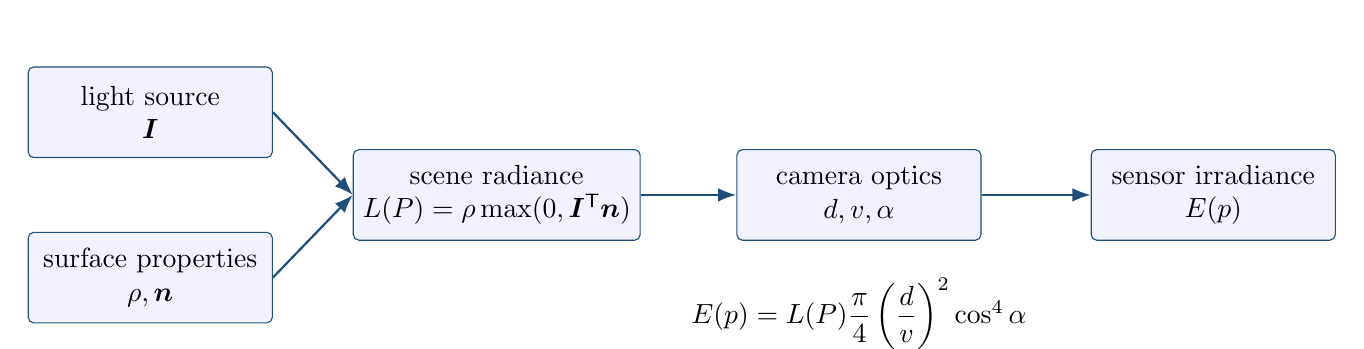
\begin{tikzpicture}[
  >=Latex,
  stage/.style={draw=noteBlue,rounded corners=2pt,fill=blue!5,
    minimum width=3.1cm,minimum height=1.15cm,align=center},
  flow/.style={->,thick,draw=noteBlue}
]
  \node[stage] (light) at (0,1.05) {light source\\$\bm I$};
  \node[stage] (surface) at (0,-1.05) {surface properties\\$\rho,\bm n$};
  \node[stage] (radiance) at (4.4,0) {scene radiance\\$L(P)=\rho\max(0,\bm I^{\mathsf T}\bm n)$};
  \node[stage] (optics) at (9.0,0) {camera optics\\$d,v,\alpha$};
  \node[stage] (irradiance) at (13.5,0) {sensor irradiance\\$E(p)$};

  \draw[flow] (light.east) -- (radiance.west);
  \draw[flow] (surface.east) -- (radiance.west);
  \draw[flow] (radiance) -- (optics);
  \draw[flow] (optics) -- (irradiance);

  \node[below=0.35cm of optics,align=center]
    {$E(p)=L(P)\dfrac{\pi}{4}\left(\dfrac{d}{v}\right)^2\cos^4\alpha$};
\end{tikzpicture}
}
  \caption{Photometric image formation（光度成像）的两个阶段：表面产生 radiance，光学系统把它转换为 sensor irradiance。}
  \label{fig:sc4061-l01-photometry}
\end{figure}

在讲义采用的理想模型中，sensor point（传感器点）$p$ 的 irradiance（辐照度）为
\[
  E(p)=L(P)\frac{\pi}{4}\left(\frac{d}{v}\right)^2\cos^4\alpha,
\]
其中 $d$ 是 aperture diameter（光圈直径），$v$ 是 image distance（像距），$\alpha$ 是光线相对 optical axis（光轴）的夹角。该式说明进光量近似随 $d^2$ 增加，离轴位置因 $\cos^4\alpha$ 出现 vignetting（暗角）。

更常用的简化表达是
\[
  f(x,y)=i(x,y)r(x,y),
\]
其中 $i$ 为 illumination（光照），$r$ 为 reflectance（反射率）。只观察 $f$ 无法唯一分离 $i$ 与 $r$，这正是 inverse problem（逆问题）的一个具体来源。

\lecturetopic{SC4061-L01-T06}{Sensor、Sampling、Quantization 与 Image Matrix}

Sensor array（传感器阵列）由二维 photo-detectors（光电探测器）组成。每个探测器记录的信号与 exposure（曝光量）相关：
\[
  \text{exposure}=\text{irradiance}\times\text{exposure time}.
\]
单个探测器主要测量强度；Bayer mask（拜耳滤色阵列）让不同位置分别采集 R/G/B（红/绿/蓝）通道，再通过 demosaicing（去马赛克）估计每个 pixel（像素）的完整颜色。

\begin{figure}[htbp]
  \centering
  \resizebox{0.94\textwidth}{!}{\begin{tikzpicture}[>=Latex,font=\small]
  % Sampling panel.
  \begin{scope}
    \draw[->] (0,0) -- (5.4,0) node[right] {$x$};
    \draw[->] (0,0) -- (0,3.6) node[above] {intensity};
    \draw[very thick,draw=orange!90!black,smooth]
      plot coordinates {(0.25,0.55) (0.8,1.25) (1.35,0.9) (1.9,2.35)
                        (2.45,1.55) (3.0,3.05) (3.55,1.25) (4.1,2.15)
                        (4.65,1.65) (5.05,2.65)};
    \foreach \x/\y in {0.5/0.85,1.1/1.05,1.7/1.8,2.3/1.7,2.9/2.8,3.5/1.3,4.1/2.15,4.7/1.75}{
      \draw[->,draw=noteBlue] (\x,0) -- (\x,\y);
      \fill[noteBlue] (\x,\y) circle (1.8pt);
    }
    \node[below=0.55cm,align=center] at (2.7,0)
      {sampling（采样）\\$x=m\Delta x$};
  \end{scope}

  \draw[->,very thick,draw=ntuRed] (5.9,1.8) -- node[above] {$Q(\cdot)$} (7.1,1.8);

  % Quantization panel.
  \begin{scope}[xshift=7.5cm]
    \draw[->] (0,0) -- (5.4,0) node[right] {$m$};
    \draw[->] (0,0) -- (0,3.6) node[above] {level};
    \foreach \y in {0.8,1.6,2.4,3.2}{
      \draw[dotted,draw=gray] (0,\y) -- (5.1,\y);
    }
    \foreach \x/\y in {0.5/0.8,1.1/0.8,1.7/1.6,2.3/1.6,2.9/3.2,3.5/1.6,4.1/2.4,4.7/1.6}{
      \draw[->,draw=noteBlue] (\x,0) -- (\x,\y);
      \fill[noteBlue] (\x,\y) circle (1.8pt);
    }
    \node[below=0.55cm,align=center] at (2.7,0)
      {quantization（量化）\\continuous value $\rightarrow$ finite levels};
  \end{scope}
\end{tikzpicture}
}
  \caption{Sampling（采样）离散化空间位置，quantization（量化）把测量值映射到有限灰度等级。}
  \label{fig:sc4061-l01-sampling-quantization}
\end{figure}

二维数字化过程可统一写成
\[
  \boxed{g[m,n]=Q\!\left(f(m\Delta x,n\Delta y)\right)}.
\]
Sampling interval（采样间隔）过大会丢失空间细节并引发 aliasing（混叠）；quantization levels（量化等级）过少会产生 banding（色带）或明显的强度跳变。$b$-bit quantization（$b$ 位量化）共有 $2^b$ 个等级，例如 8-bit 灰度通常为 $0$--$255$。

Grayscale image（灰度图像）可视为 scalar function（标量函数）$f(x,y)$ 或二维矩阵；RGB image（彩色图像）可视为三个通道组成的三维数组。代码中通常采用
\[
  \boxed{I[\text{row},\text{column}]=I[y,x]},
\]
即 $x$ 对应 column（列），$y$ 对应 row（行）。Python/NumPy 通常从 0 编号，MATLAB 通常从 1 编号。

PNG/TIFF 常用于 lossless representation（无损表示），JPEG 使用 lossy compression（有损压缩），JPEG~2000 使用 wavelet-based compression（基于小波的压缩）。文件大小不能只由 pixel count（像素数）决定，还必须说明 channel count（通道数）、bit depth（位深）和 compression（压缩方式）。

\textbf{对应例题：}\relatedexercise{SC4061-L01-E02}{Sampling、Quantization 与存储量}。

\subsection{一分钟回顾}

三维 scene（场景）先通过 lighting 与 reflection（光照与反射）产生 radiance（辐亮度），再由 lens 和 aperture（透镜和光圈）映射为 sensor irradiance（传感器辐照度），最后经 sampling 与 quantization（采样与量化）成为 image matrix（图像矩阵）。Thin lens equation（薄透镜公式）描述几何成像；aperture（光圈）同时影响亮度和 depth of field（景深）；pixel intensity（像素强度）并不等于物体固有属性。Computer Vision（计算机视觉）则试图沿这条链反向推断场景。

% Actual class: 02
% Slide deck: L1 Imaging v1 full
% Exact scope: pp. 25--40; L1_MATLAB.m, all sections
% NTULearn supplement: L1 Part 3 and MATLAB Demo transcripts
% Human verified: Yes

\section{第 02 节课：Extended Imaging、Perceptron 与 MATLAB Image Operations}
\label{lecture:SC4061-L02}

\lecturemeta
  {SC4061-L02}
  {2026-08-18}
  {L1 Imaging v1 full；L1\_MATLAB.m}
  {L1 pp.~25--40；MATLAB 示例全部内容}
  {课程视频 L1 Part 3 与 MATLAB Demo（字幕核对）}
  {已确认（2026-08-18）}

\subsection{本讲主线}

本讲从 traditional camera（传统相机）扩展到 computational imaging（计算成像）与其他 sensing modalities（传感模态），随后用 Perceptron（感知机）说明如何从 labelled samples（带标签样本）学习 decision boundary（决策边界）。MATLAB 部分把 image（图像）视为数组，并用 subsampling（下采样）和 logical mask（逻辑掩膜）完成最基本的图像操作。

\lecturetopic{SC4061-L02-T01}{Beyond a Conventional 2D Camera}

\begin{center}
\small
\begin{tabularx}{\textwidth}{@{}>{\raggedright\arraybackslash}p{3.5cm}>{\raggedright\arraybackslash}p{4.2cm}>{\raggedright\arraybackslash}X@{}}
  \toprule
  Imaging method（成像方式） & Measurement（测量量） & 关键结论 \\
  \midrule
  Light-field camera（光场相机） & lenslet array（微透镜阵列）采样光线的位置与方向 & 可进行 post-capture refocusing（拍摄后重聚焦），代价是数据量与空间分辨率折衷 \\
  LiDAR（激光雷达） & laser pulse（激光脉冲）的 round-trip time of flight（往返飞行时间） & 估计 depth（深度），常得到 sparse point cloud（稀疏点云） \\
  Ultrasound（超声） & 声波回波 & 不依赖可见光，可用于体内结构成像 \\
  X-ray / CT（X 射线/计算机断层成像） & X 射线穿透后的 attenuation（衰减） & radiograph（投影片）给出二维投影；CT 由多角度投影重建截面或三维体数据 \\
  MRI（磁共振成像） & magnetic resonance signal（磁共振信号） & 形成体数据，不使用 ionizing X-ray（电离 X 射线） \\
  \bottomrule
\end{tabularx}
\end{center}

LiDAR 的理想 range equation（测距公式）为
\[
  \boxed{d=\frac{c\,\Delta t}{2}},
\]
其中 $c$ 是光速，$\Delta t$ 是 round-trip time（往返时间）。除以 $2$ 是因为脉冲走过的总路程是 $2d$。

\begin{figure}[htbp]
  \centering
  \resizebox{0.82\textwidth}{!}{\begin{tikzpicture}[>=Latex,font=\small]
  \node[draw=noteBlue,rounded corners=2pt,fill=blue!5,
    minimum width=2.5cm,minimum height=1.6cm,align=center] (sensor)
    {emitter + receiver\\（发射器与接收器）};
  \node[draw=ntuRed,very thick,minimum width=0.25cm,minimum height=3.0cm,
    right=8.6cm of sensor] (target) {};
  \node[right=0.2cm of target,align=left] {object surface\\（物体表面）};

  \draw[->,very thick,draw=ntuRed]
    ([yshift=0.42cm]sensor.east) -- node[above]{emitted pulse（发射脉冲）} ([yshift=0.42cm]target.west);
  \draw[->,very thick,draw=noteBlue]
    ([yshift=-0.42cm]target.west) -- node[below]{returned pulse（返回脉冲）} ([yshift=-0.42cm]sensor.east);

  \draw[<->,draw=gray,thick]
    ([yshift=-1.45cm]sensor.east) -- node[fill=white,inner sep=2pt] {$d$} ([yshift=-1.45cm]target.west);
  \node[below=0.72cm of sensor,align=center]
    {$t_0$：send\\$t_0+\Delta t$：receive};
  \node[below=1.0cm of target,anchor=east,align=right]
    {$2d=c\Delta t$\\$d=c\Delta t/2$};
\end{tikzpicture}
}
  \caption{Time-of-Flight（飞行时间）测距：同一个传感器记录 pulse（脉冲）的发射与返回时刻。}
  \label{fig:sc4061-l02-tof}
\end{figure}

\textbf{对应例题：}\relatedexercise{SC4061-L02-E02}{LiDAR Time-of-Flight 测距}。

\lecturetopic{SC4061-L02-T02}{Perceptron as a Linear Classifier}

将 bias（偏置）吸收到增广向量中：
\[
  \tilde{\bm x}=\begin{bmatrix}\bm x\\1\end{bmatrix},
  \qquad
  \tilde{\bm w}=\begin{bmatrix}\bm w\\b\end{bmatrix},
  \qquad
  s=\tilde{\bm w}^{\mathsf T}\tilde{\bm x}.
\]
Perceptron 使用 weighted sum（加权和）与 threshold（阈值）分类：$s>0$ 判为 $C_1$，$s<0$ 判为 $C_2$；$s=0$ 构成 decision boundary：
\[
  \boxed{\tilde{\bm w}^{\mathsf T}\tilde{\bm x}=0}.
\]
二维时它是一条直线，高维时是 hyperplane（超平面）。Weights（权重）改变边界的方向，bias 改变边界的位置。

\lecturetopic{SC4061-L02-T03}{Perceptron Learning Rule}

给定 learning rate（学习率）$\alpha>0$，仅在样本被误分类或恰好落在边界上时更新：
\[
\tilde{\bm w}(k+1)=
\begin{cases}
\tilde{\bm w}(k)+\alpha\tilde{\bm x}(k),
  & \tilde{\bm x}(k)\in C_1,\ s(k)\le 0,\\
\tilde{\bm w}(k)-\alpha\tilde{\bm x}(k),
  & \tilde{\bm x}(k)\in C_2,\ s(k)\ge 0,\\
\tilde{\bm w}(k), & \text{otherwise}.
\end{cases}
\]
每次更新都会提高当前误分类样本在正确方向上的 score（得分）。但 convergence（收敛）只在 linearly-separable（线性可分）数据上有保证；即使收敛，得到的分界线也不一定具有最大 margin（间隔）。

\textbf{对应例题：}\relatedexercise{SC4061-L02-E01}{Perceptron 权重更新}。

\newpage
\lecturetopic{SC4061-L02-T04}{From Perceptron to Multi-layer Neural Networks}

Single perceptron（单个感知机）只能产生一个 linear decision boundary（线性决策边界），因此不能表示 XOR：移动或旋转一条直线都无法把对角分布的两类点完全分开。

\begin{figure}[htbp]
  \centering
  \resizebox{0.9\textwidth}{!}{\begin{tikzpicture}[>=Latex,font=\small]
  \begin{scope}
    \draw[->] (-0.25,0) -- (4.0,0) node[right] {$x_1$};
    \draw[->] (0,-0.25) -- (0,4.0) node[above] {$x_2$};
    \draw[very thick,draw=noteBlue] (0,3) -- (3,0)
      node[pos=0.58,above right,rotate=-45] {$x_1+x_2-3=0$};
    \fill[ntuRed] (3,3) circle (3pt) node[above right] {$C_1$};
    \draw[very thick,draw=noteBlue,fill=white] (1,1) circle (3pt) node[below left] {$C_2$};
    \node[align=center] at (1.9,-0.75) {linearly separable\\（线性可分）};
  \end{scope}

  \begin{scope}[xshift=7.0cm,scale=2.15]
    \draw[->] (-0.15,0) -- (1.55,0) node[right] {$x_1$};
    \draw[->] (0,-0.15) -- (0,1.55) node[above] {$x_2$};
    \fill[ntuRed] (0,1) circle (1.5pt);
    \fill[ntuRed] (1,0) circle (1.5pt);
    \draw[very thick,draw=noteBlue,fill=white] (0,0) circle (1.5pt);
    \draw[very thick,draw=noteBlue,fill=white] (1,1) circle (1.5pt);
    \draw[dashed,draw=gray] (-0.05,0.55) -- (1.2,0.55);
    \draw[dashed,draw=gray] (0.55,-0.05) -- (0.55,1.2);
    \node[scale=0.48,align=center] at (0.62,-0.38) {XOR: no single line works\\（不存在单一直线分隔）};
    \node[scale=0.48,text=ntuRed,anchor=west] at (1.18,1.18) {$C_1$: output 1};
    \node[scale=0.48,text=noteBlue,anchor=west] at (1.18,0.96) {$C_2$: output 0};
  \end{scope}
\end{tikzpicture}
}
  \caption{左：线性可分样本可由一个 Perceptron 分类；右：XOR 不存在单一直线分隔。}
  \label{fig:sc4061-l02-perceptron-xor}
\end{figure}

另一种训练思路是显式最小化 squared-error loss（平方误差损失）：
\[
  E(\bm w)=\frac12\left(r-\bm w^{\mathsf T}\bm x\right)^2,
  \qquad
  \boxed{\bm w(k+1)=\bm w(k)+\alpha
  \left[r(k)-\bm w^{\mathsf T}(k)\bm x(k)\right]\bm x(k)}.
\]
这来自 gradient descent（梯度下降）$\bm w\leftarrow\bm w-\alpha\nabla E$。与基于“是否分错”的第一种规则相比，它直接根据 prediction error（预测误差）的大小更新权重。

Multi-layer neural network（多层神经网络）把多个 neurons（神经元）分层连接，并在层间加入 nonlinear activation（非线性激活），从而组合出非线性边界。若各层之间没有非线性激活，多层线性变换仍等价于单个线性变换，不能解决 XOR。Training（训练）通常包括：
\[
\begin{aligned}
  \text{forward pass（前向传播）}
  &\longrightarrow \text{loss（损失）}\\
  &\longrightarrow \text{backpropagation（反向传播）}
  \longrightarrow \text{weight update（权重更新）}.
\end{aligned}
\]
Backpropagation 本质上用 chain rule（链式法则）高效计算各层参数的 gradient（梯度）。本课程在此只建立概念联系，不要求从零搭建完整神经网络。

\lecturetopic{SC4061-L02-T05}{MATLAB: Images Are Arrays}

MATLAB 默认以 radians（弧度）解释三角函数参数，因此
\[
  \texttt{sin(30)}\ne 0.5,
  \qquad
  \texttt{sin(30/180*pi)}=0.5.
\]
在 script（脚本）中，分号抑制命令行输出，\texttt{\%} 开始注释，\texttt{\%\%} 划分可单独运行的 section（代码节）。

\begin{center}
\small
\begin{tabularx}{\textwidth}{@{}lX@{}}
  \toprule
  MATLAB expression（表达式） & 含义 \\
  \midrule
  \texttt{a=imread('Singapore.jpg')} & 读取本地 RGB image；本次示例得到 $600\times1280\times3$ 的 \texttt{uint8} array（数组） \\
  \texttt{a(i,j,c)} & 第 $i$ 行、第 $j$ 列、第 $c$ 个 channel（通道）；索引顺序是 row, column, channel \\
  \texttt{a(i,j,:)} & 取一个 pixel（像素）的全部 RGB 分量 \\
  \texttt{a(1:s:end,1:s:end,:)} & 两个空间方向每隔 $s$ 个像素取样，保留全部通道 \\
  \bottomrule
\end{tabularx}
\end{center}

若两个方向都采用 stride（步长）$s$，高度和宽度约缩为原来的 $1/s$，pixel count（像素数）约缩为 $1/s^2$。这是 lossy downsampling（有损下采样），并不等同于一般的 image compression（图像压缩）；只有把结果重新编码保存后，文件大小才会相应变化。

\lecturetopic{SC4061-L02-T06}{Logical Mask 与 Vectorized Operation}

课程示例把满足 $R+G+B>300$ 的 bright pixels（亮像素）置为 $(60,60,60)$。先把 \texttt{uint8} image 转为 \texttt{double} 可避免整数运算的范围限制：
\[
  M(i,j)=\mathbf 1\!\left[R(i,j)+G(i,j)+B(i,j)>300\right].
\]
然后对每个 channel $c$ 统一更新：
\[
  B_c=A_c(1-M)+60M.
\]

\begin{figure}[htbp]
  \centering
  \resizebox{\textwidth}{!}{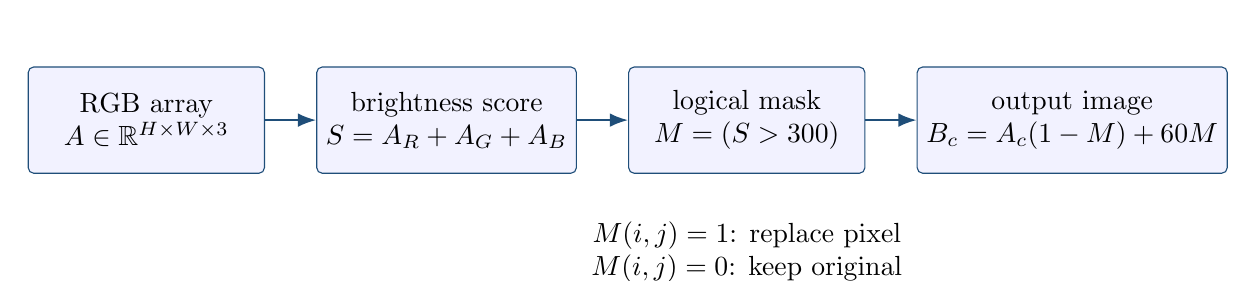
\begin{tikzpicture}[
  >=Latex,
  stage/.style={draw=noteBlue,rounded corners=2pt,fill=blue!5,
    minimum width=3.0cm,minimum height=1.35cm,align=center},
  flow/.style={->,thick,draw=noteBlue}
]
  \node[stage] (rgb) {RGB array\\$A\in\mathbb{R}^{H\times W\times3}$};
  \node[stage,right=0.65cm of rgb] (score) {brightness score\\$S=A_R+A_G+A_B$};
  \node[stage,right=0.65cm of score] (mask) {logical mask\\$M=(S>300)$};
  \node[stage,right=0.65cm of mask] (output) {output image\\$B_c=A_c(1-M)+60M$};

  \draw[flow] (rgb) -- (score);
  \draw[flow] (score) -- (mask);
  \draw[flow] (mask) -- (output);

  \node[below=0.48cm of mask,align=center]
    {$M(i,j)=1$: replace pixel\\$M(i,j)=0$: keep original};
\end{tikzpicture}
}
  \caption{Logical mask（逻辑掩膜）把 pixel-wise condition（逐像素条件）与批量赋值分开。}
  \label{fig:sc4061-l02-matlab-mask}
\end{figure}

Vectorized operation（向量化运算）把循环交给 MATLAB 的底层数组实现，通常比解释执行的双重 \texttt{for} loop 更快，也更接近公式表达；具体加速倍数取决于 MATLAB 版本、硬件和数组大小，不能把单次计时当作固定结论。

\textbf{对应例题：}\relatedexercise{SC4061-L02-E03}{RGB Threshold 与 Logical Mask}。

% Actual class: 03
% Slide deck: L2 (full) Spatial slides
% Exact scope: pp. 1--40
% NTULearn supplement: three L2 video transcripts, Parts 1--3
% Human verified: Yes

\section{第 03 节课：Spatial-domain Enhancement、Filtering 与 CNN}
\label{lecture:SC4061-L03}

\lecturemeta
  {SC4061-L03}
  {2026-08-25}
  {L2 (full) Spatial slides}
  {L2 pp.~1--40（Parts 1--3 全部）}
  {课程视频 L2 Parts 1--3（字幕核对）}
  {已确认（2026-08-25）}

\subsection{本讲主线}

Image enhancement（图像增强）不创造新的 scene information（场景信息），而是通过重新分配 intensity（灰度）或利用 neighbourhood（邻域）让已有结构更容易被人或算法识别。本讲先比较 point processing（点处理）与 spatial filtering（空间滤波），再说明 CNN（卷积神经网络）如何把人工设计 kernel（核）推广为从数据中学习 kernel。

\lecturetopic{SC4061-L03-T01}{Point Processing 与 Spatial Filtering}

\begin{center}
\small
\begin{tabularx}{\textwidth}{@{}>{\raggedright\arraybackslash}p{3.2cm}>{\raggedright\arraybackslash}p{4.2cm}X@{}}
  \toprule
  Method（方法） & Output dependency（输出依赖） & 典型用途 \\
  \midrule
  Point processing（点处理） & $g(x,y)=T(f(x,y))$；输出位置不直接读取邻域，但 $T$ 的参数可以来自整幅图像的 minimum、maximum 或 histogram（直方图） & contrast stretching（对比度拉伸）、power-law transformation（幂律变换）、histogram equalisation（直方图均衡化） \\
  Spatial filtering（空间滤波） & 输出由当前位置及 neighbourhood 共同决定 & smoothing（平滑）、noise removal（去噪）、feature detection（特征检测） \\
  \bottomrule
\end{tabularx}
\end{center}

\begin{figure}[htbp]
  \centering
  \resizebox{0.94\textwidth}{!}{\begin{tikzpicture}[
  >=Latex,
  box/.style={draw=noteBlue, rounded corners=2pt, minimum width=2.5cm,
    minimum height=1.2cm, align=center, fill=blue!4},
  op/.style={draw=ntuRed, rounded corners=2pt, minimum width=2.2cm,
    minimum height=1.0cm, align=center, fill=red!4},
  every node/.style={font=\small}
]
  \node[box] (pixel) at (0,1.6) {current pixel\\$r=f(x,y)$};
  \node[op] (point) at (4.0,1.6) {point transform\\$s=T(r)$};
  \node[box] (pointout) at (8.0,1.6) {output pixel\\$g(x,y)=s$};
  \draw[->,thick] (pixel) -- (point);
  \draw[->,thick] (point) -- (pointout);
  \node[above=2pt of point] {Point processing（点处理）};

  \node[box] (neigh) at (0,-1.2) {$3\times3$ neighbourhood\\around $f(x,y)$};
  \node[op] (kernel) at (4.0,-1.2) {kernel $w$\\multiply and sum};
  \node[box] (filterout) at (8.0,-1.2) {filtered pixel\\$g(x,y)$};
  \draw[->,thick] (neigh) -- (kernel);
  \draw[->,thick] (kernel) -- (filterout);
  \node[above=2pt of kernel] {Spatial filtering（空间滤波）};
\end{tikzpicture}
}
  \caption{Point processing 只把当前 intensity 送入固定变换；spatial filtering 则让 kernel 与 neighbourhood 做逐元素运算。}
  \label{fig:sc4061-l03-enhancement-operators}
\end{figure}

\keyidea{``Pixel-wise（逐像素）''描述输出的局部依赖关系，不代表变换参数一定不使用 global statistics（全局统计量）。}

\lecturetopic{SC4061-L03-T02}{Contrast、Gamma 与 Histogram Equalisation}

若主要灰度位于 $[r_{\min},r_{\max}]$，把它线性展开到 $[0,L-1]$：
\[
  s=
  \begin{cases}
    0, & r\le r_{\min},\\[2pt]
    (L-1)\dfrac{r-r_{\min}}{r_{\max}-r_{\min}},
      & r_{\min}<r<r_{\max},\\[7pt]
    L-1, & r\ge r_{\max}.
  \end{cases}
\]
Contrast stretching 扩大有用区域的 dynamic range（动态范围），但两端的 clipping（截断）会把不同输入合并为同一输出，因此可能丢失信息。

Power-law transformation 写成
\[
  s=cr^\gamma.
\]
若要求 $r=L-1$ 仍映射到 $s=L-1$，则
\[
  \boxed{s=(L-1)\left(\frac{r}{L-1}\right)^\gamma},
  \qquad c=(L-1)^{1-\gamma}.
\]
$\gamma<1$ 提升 dark pixels（暗像素），$\gamma>1$ 相对突出 bright region（亮部区域），$\gamma=1$ 为 identity mapping（恒等映射）。

\begin{figure}[htbp]
  \centering
  \resizebox{0.9\textwidth}{!}{\begin{tikzpicture}[>=Latex,every node/.style={font=\small}]
  \begin{scope}[xshift=0cm]
    \draw[->] (0,0) -- (4.5,0) node[right] {$r$};
    \draw[->] (0,0) -- (0,4.5) node[above] {$s$};
    \draw[very thick,ntuRed] (0,0) -- (0.9,0) -- (3.2,4) -- (4.1,4);
    \draw[densely dashed] (0.9,0) -- (0.9,-0.18) node[below] {$r_{\min}$};
    \draw[densely dashed] (3.2,4) -- (3.2,-0.18) node[below] {$r_{\max}$};
    \node[align=center] at (2.05,4.75) {contrast stretching\\（对比度拉伸）};
  \end{scope}

  \begin{scope}[xshift=6.2cm]
    \draw[->] (0,0) -- (4.5,0) node[right] {$r$};
    \draw[->] (0,0) -- (0,4.5) node[above] {$s$};
    \draw[densely dashed,gray] (0,0) -- (4,4);
    \draw[very thick,noteBlue,domain=0:4,samples=40]
      plot (\x,{4*sqrt(\x/4)});
    \draw[very thick,ntuRed,domain=0:4,samples=40]
      plot (\x,{4*(\x/4)*(\x/4)});
    \node[noteBlue,anchor=west] at (2.6,3.45) {$\gamma<1$};
    \node[ntuRed,anchor=west] at (2.7,1.25) {$\gamma>1$};
    \node[gray,anchor=west] at (2.7,2.55) {$\gamma=1$};
    \node[align=center] at (2.05,4.75) {power-law mapping\\（幂律映射）};
  \end{scope}
\end{tikzpicture}
}
  \caption{三类 intensity mapping（灰度映射）的形状。纵横轴均表示归一化后的输出/输入灰度。}
  \label{fig:sc4061-l03-intensity-mappings}
\end{figure}

Histogram equalisation 用 cumulative distribution function, CDF（累积分布函数）自动构造单调映射。若图像大小为 $M\times N$、gray level（灰度级）数为 $L$，且 $n_j$ 个像素取值为 $r_j$，则
\[
  p_r(r_j)=\frac{n_j}{MN},
  \qquad
  \boxed{s_k=\operatorname{round}\!\left((L-1)\sum_{j=0}^{k}p_r(r_j)\right)}.
\]
最后一个 CDF 值为 $1$，故最大灰度映射到 $L-1$。离散情形下结果只会\emph{近似}均匀：一个 input bin（输入灰度箱）不能被确定性映射拆开，而多个 input bins 可以合并到同一个 output bin。CDF 单调不减，因此灰度顺序不会反转。

\textbf{对应例题：}
\begin{itemize}
  \item \relatedexercise{SC4061-L03-E01}{Contrast Stretching 数值计算}；
  \item \relatedexercise{SC4061-L03-E02}{Histogram Equalisation 映射}。
\end{itemize}

\lecturetopic{SC4061-L03-T03}{Correlation、Convolution 与 Padding}

对大小为 $(2a+1)\times(2b+1)$ 的 kernel $w$，讲义采用的 correlation（相关）定义为
\[
  \boxed{g(x,y)=\sum_{u=-a}^{a}\sum_{v=-b}^{b}
  f(x+u,y+v)w(u,v)}.
\]
它把 neighbourhood 与 kernel 做 element-wise multiplication（逐元素相乘）后求和。Convolution（卷积）先将 kernel 旋转 $180^\circ$：
\[
  h(u,v)=w(-u,-v),
  \qquad
  g(x,y)=\sum_{u=-a}^{a}\sum_{v=-b}^{b}f(x-u,y-v)h(u,v).
\]
一般 asymmetric kernel（非对称核）会使二者结果不同；若 $w(u,v)=w(-u,-v)$，则 kernel 旋转后不变，二者在相同 boundary handling（边界处理）下结果相同。

Border pixels（边界像素）缺少完整邻域，需要 padding（填充）。Zero padding（零填充）简单但可能产生不自然的 dark border（暗边）；replication（边界复制）和 mirror padding（镜像填充）通常能更平滑地延续边界结构。

\textbf{对应例题：}
\relatedexercise{SC4061-L03-E03}{Correlation 与 Kernel Rotation}。

\lecturetopic{SC4061-L03-T04}{Box、Gaussian 与 Median Filtering}

\textbf{Box/Average filter（方框/均值滤波器）}对邻域等权平均。例如
\[
  w=\frac{1}{9}
  \begin{bmatrix}
    1&1&1\\1&1&1\\1&1&1
  \end{bmatrix}.
\]
若 $X_i=S+N_i$，其中 $N_i$ 相互 independent（独立）、均值为 $0$、方差为 $\sigma^2$，对 $n$ 个观测平均后
\[
  E[\bar X]=S,
  \qquad
  \operatorname{Var}(\bar X)=\frac{\sigma^2}{n},
  \qquad
  \operatorname{Std}(\bar X)=\frac{\sigma}{\sqrt n}.
\]
若 noise（噪声）相关，则方差不能直接写成 $\sigma^2/n$；若相邻信号并不近似相同，平均还会模糊 edge（边缘）。

\textbf{Gaussian filter（高斯滤波器）}让靠近中心的像素贡献更大：
\[
  h(x,y)=\frac{1}{2\pi\sigma^2}
  \exp\!\left(-\frac{x^2+y^2}{2\sigma^2}\right),
\]
离散化后需归一化使 kernel weights（核权重）之和为 $1$。$\sigma$ 控制权重的空间扩散范围。

\textbf{Median filter（中值滤波器）}把邻域值排序后取中位数，不是 weighted sum，因此是 non-linear filter（非线性滤波器）。它特别适合 impulse/salt-and-pepper noise（脉冲/椒盐噪声），通常比均值滤波更能保留 edge。

\begin{remark}
讲义把 speckle noise（散斑噪声）与 impulse/salt-and-pepper noise 并列为同义表述并不严谨。Speckle 通常是 coherent imaging（相干成像）中的 multiplicative granular noise（乘性颗粒噪声），不等同于离散的椒盐噪声。
\end{remark}

\textbf{对应例题：}
\relatedexercise{SC4061-L03-E04}{Noise Averaging 与 Median Filtering}。

\lecturetopic{SC4061-L03-T05}{从 Local Average 到 Similarity-based Denoising}

Spatial averaging（空间平均）并不必须只使用几何上相邻的 pixels；更一般的策略是寻找 appearance 或 structure（结构）相似的区域：
\begin{itemize}
  \item Bilateral filter（双边滤波）同时考虑 spatial distance（空间距离）与 intensity similarity（灰度相似度）；
  \item Non-local Means, NLM（非局部均值）在更大范围内搜索 similar patches（相似图像块）；
  \item BM3D 把相似 patches 组成三维数组并进行 collaborative filtering（协同滤波）。
\end{itemize}
这些内容在本讲属于 extended reading（扩展阅读）；重点是理解``按相似性聚合''相较固定局部平均更可能保留重复结构。

\lecturetopic{SC4061-L03-T06}{From Hand-crafted Kernels to Learned Kernels}

Traditional image processing（传统图像处理）根据任务手工指定 kernel；复杂任务中，每个 weight 很难由人直接设计。CNN 预先规定 network structure（网络结构），再通过 training data（训练数据）、forward propagation（前向传播）、backpropagation（反向传播）和 optimization（优化）学习 kernel weights。

同一 kernel 在不同位置重复使用称为 weight sharing（权重共享），使同一种 local feature（局部特征）可以在整幅图像上被检测，并大幅减少参数数量。严格来说，大多数 deep-learning frameworks 中名为 ``convolution'' 的运算不旋转 kernel，数学上是 cross-correlation（互相关）；由于 kernel 本身可学习，这一命名约定不削弱模型的表达能力，但考试中仍需区分两种定义。

\begin{figure}[htbp]
  \centering
  \resizebox{0.96\textwidth}{!}{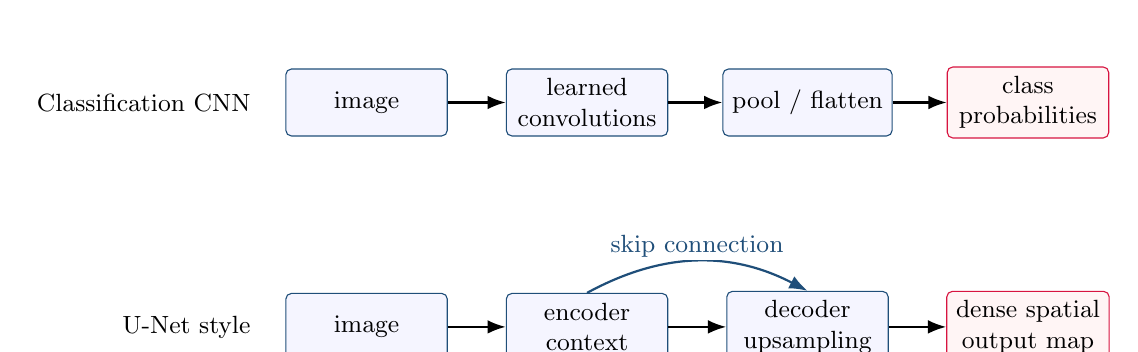
\begin{tikzpicture}[
  >=Latex,
  stage/.style={draw=noteBlue, rounded corners=2pt, minimum width=2.05cm,
    minimum height=0.85cm, align=center, fill=blue!4},
  dense/.style={draw=ntuRed, rounded corners=2pt, minimum width=2.05cm,
    minimum height=0.85cm, align=center, fill=red!4},
  every node/.style={font=\small}
]
  \node[stage] (im1) at (0,1.6) {image};
  \node[stage] (conv1) at (2.8,1.6) {learned\\convolutions};
  \node[stage] (pool1) at (5.6,1.6) {pool / flatten};
  \node[dense] (class) at (8.4,1.6) {class\\probabilities};
  \draw[->,thick] (im1)--(conv1);
  \draw[->,thick] (conv1)--(pool1);
  \draw[->,thick] (pool1)--(class);
  \node[anchor=east] at (-1.35,1.6) {Classification CNN};

  \node[stage] (im2) at (0,-1.25) {image};
  \node[stage] (enc) at (2.8,-1.25) {encoder\\context};
  \node[stage] (dec) at (5.6,-1.25) {decoder\\upsampling};
  \node[dense] (map) at (8.4,-1.25) {dense spatial\\output map};
  \draw[->,thick] (im2)--(enc);
  \draw[->,thick] (enc)--(dec);
  \draw[->,thick] (dec)--(map);
  \draw[->,thick,noteBlue,bend left=28] (enc.north) to
    node[above,fill=white,inner sep=1pt] {skip connection} (dec.north);
  \node[anchor=east] at (-1.35,-1.25) {U-Net style};
\end{tikzpicture}
}
  \caption{Classification CNN（上）把 spatial features 压缩为类别；U-Net 式 dense prediction（下）利用 decoder 与 skip connections 恢复逐像素输出。}
  \label{fig:sc4061-l03-cnn-pipeline}
\end{figure}

\lecturetopic{SC4061-L03-T07}{LeNet、AlexNet 与 U-Net}

\begin{center}
\small
\begin{tabularx}{\textwidth}{@{}>{\raggedright\arraybackslash}p{2cm}>{\raggedright\arraybackslash}p{3.5cm}X@{}}
  \toprule
  Network（网络） & Output/task（输出/任务） & 本讲应掌握的意义 \\
  \midrule
  LeNet & handwritten digit/document recognition（手写数字/文档识别） & 早期成功组合 learned convolution、subsampling 与 backpropagation \\
  AlexNet & ImageNet classification（图像分类） & 2012 年以更深的网络显著推动 deep learning 在视觉任务中的应用 \\
  U-Net & segmentation、denoising 等 image-to-image tasks（图像到图像任务） & Encoder（编码器）提取 context，decoder（解码器）恢复空间分辨率，skip connections（跳跃连接）传递高分辨率细节 \\
  \bottomrule
\end{tabularx}
\end{center}

普通 classification CNN 最终输出一个 class label 或 class probabilities（类别概率）；U-Net 输出与输入具有 spatial correspondence（空间对应关系）的 dense map（稠密图），适合 pixel-level prediction（逐像素预测）。这一性质适用于视觉中的 segmentation、denoising、depth estimation 等任务，不能直接等同于 natural-language sequence generation（自然语言序列生成）。

\subsection{一分钟回顾}

Point processing 通过 $s=T(r)$ 重新分配 intensity，其中 histogram equalisation 用 CDF 自动构造单调映射；spatial filtering 用 neighbourhood 与 kernel 进行 correlation 或 convolution。Box 与 Gaussian filter 是 linear smoothing（线性平滑），median filter 是适合 impulse noise 的 nonlinear filter。CNN 把人工 kernel 改为 learned kernel，并依靠 weight sharing 复用局部检测器；classification CNN 输出类别，而 U-Net 通过 encoder--decoder 与 skip connections 产生 dense spatial output。

% Actual class: 04
% Slide deck: L3 (full) Frequency slides
% Exact scope: pp. 1--32 (Parts 1--2)
% NTULearn supplement: two L3 video transcripts; test2_FT.m
% Human verified: Yes

\section{第 04 节课：Frequency-domain Image Enhancement}
\label{lecture:SC4061-L04}

\lecturemeta
  {SC4061-L04}
  {2026-09-01}
  {L3 (full) Frequency slides；\texttt{test2\_FT.m}}
  {L3 pp.~1--32（Parts 1--2）；pp.~33--45 留待 Part 3}
  {课程视频 L3 Parts 1--2（字幕核对）}
  {已确认（2026-09-01）}

\subsection{本讲主线}

Frequency-domain processing（频域处理）把 image（图像）分解为不同 spatial frequency（空间频率）和 orientation（方向）的 Fourier modes（傅里叶模态），修改各模态的 coefficients（系数），再合成为输出图像。它特别适合 global periodic disturbance（全局周期干扰）与按频率定义的 filtering；但 Fourier transform 始终可用不等于始终最方便，是否简化问题取决于目标 operator（算符）在 Fourier basis 中是否 diagonal 或 sparse。

\lecturetopic{SC4061-L04-T01}{Fourier Decomposition 与二维 Modes}

对 $M\times N$ image，采用 $x=0,\ldots,M-1$、$y=0,\ldots,N-1$，Fourier atom（傅里叶原子）为
\[
  \boxed{a_{u,v}(x,y)=
  \exp\!\left[j2\pi\left(\frac{ux}{M}+\frac{vy}{N}\right)\right]},
\]
其中 $u=0,\ldots,M-1$、$v=0,\ldots,N-1$ 是 mode indices（模态索引），不是脱离具体算符而独立存在的 eigenvalues（特征值）。$u/M$ 与 $v/N$ 表示 cycles per pixel（周期/像素）；相应 angular spatial frequencies（角空间频率）为 $2\pi u/M$ 与 $2\pi v/N$。

\begin{figure}[htbp]
  \centering
  \resizebox{0.94\textwidth}{!}{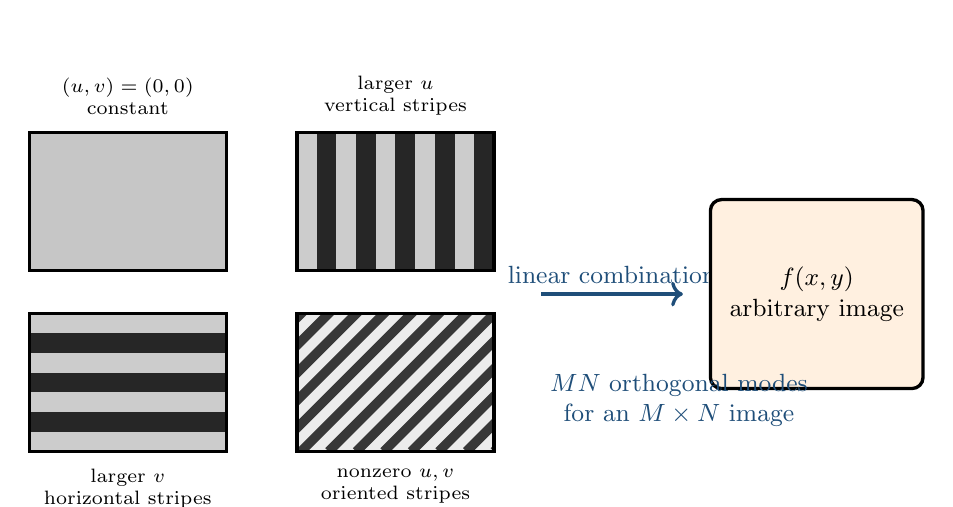
\begin{tikzpicture}[x=1cm,y=1cm,font=\small]
  \tikzset{tile/.style={draw,very thick,minimum width=2.5cm,minimum height=1.75cm}}

  \begin{scope}[shift={(0,2.3)}]
    \fill[gray!45] (0,0) rectangle (2.5,1.75);
    \draw[very thick] (0,0) rectangle (2.5,1.75);
    \node[above=1mm,align=center,font=\scriptsize] at (1.25,1.75)
      {$(u,v)=(0,0)$\\constant};
  \end{scope}

  \begin{scope}[shift={(3.4,2.3)}]
    \begin{scope}
      \clip (0,0) rectangle (2.5,1.75);
      \foreach \i in {0,...,9}{
        \pgfmathtruncatemacro{\shade}{20+65*mod(\i,2)}
        \fill[black!\shade] (0.25*\i,0) rectangle ++(0.25,1.75);
      }
    \end{scope}
    \draw[very thick] (0,0) rectangle (2.5,1.75);
    \node[above=1mm,align=center,font=\scriptsize] at (1.25,1.75)
      {larger $u$\\vertical stripes};
  \end{scope}

  \begin{scope}[shift={(0,0)}]
    \begin{scope}
      \clip (0,0) rectangle (2.5,1.75);
      \foreach \i in {0,...,6}{
        \pgfmathtruncatemacro{\shade}{20+65*mod(\i,2)}
        \fill[black!\shade] (0,0.25*\i) rectangle ++(2.5,0.25);
      }
    \end{scope}
    \draw[very thick] (0,0) rectangle (2.5,1.75);
    \node[below=1mm,align=center,font=\scriptsize] at (1.25,0)
      {larger $v$\\horizontal stripes};
  \end{scope}

  \begin{scope}[shift={(3.4,0)}]
    \fill[gray!15] (0,0) rectangle (2.5,1.75);
    \begin{scope}
      \clip (0,0) rectangle (2.5,1.75);
      \foreach \k in {-5,...,10}{
        \draw[line width=3.4pt,black!78] (-1+0.35*\k,0) -- ++(2.8,2.8);
      }
    \end{scope}
    \draw[very thick] (0,0) rectangle (2.5,1.75);
    \node[below=1mm,align=center,font=\scriptsize] at (1.25,0)
      {nonzero $u,v$\\oriented stripes};
  \end{scope}

  \draw[->,very thick,noteBlue] (6.5,2.0) -- (8.3,2.0)
    node[midway,above,align=center] {linear\ combination};
  \node[draw,very thick,rounded corners,fill=orange!12,
    minimum width=2.7cm,minimum height=2.4cm,align=center] at (10.0,2.0)
    {$f(x,y)$\\arbitrary image};
  \node[align=center,text=noteBlue] at (8.25,0.65)
    {$MN$ orthogonal modes\\for an $M\times N$ image};
\end{tikzpicture}
}
  \caption{二维 Fourier modes：$(u,v)$ 控制灰度变化的密度与方向，$MN$ 个正交 modes 构成 $M\times N$ image space 的一组完整 basis。}
  \label{fig:sc4061-l04-fourier-modes}
\end{figure}

Pixel basis（像素基）同样有 $MN$ 个 basis images：每个 basis image 仅一个 pixel 为 $1$。因此每个 pixel 是一个 coordinate（坐标），整个 image space 的维数为 $MN$；natural-image correlation（自然图像相关性）可能使真实数据集中于低维结构，但不改变 ambient vector-space dimension（环境向量空间维数）。

\lecturetopic{SC4061-L04-T02}{DFT、IDFT 与 Spectrum}

本讲采用 forward transform 不归一化、inverse transform 除以 $MN$ 的 convention：
\[
  \boxed{F(u,v)=\sum_{x=0}^{M-1}\sum_{y=0}^{N-1}
  f(x,y)\exp\!\left[-j2\pi\left(\frac{ux}{M}+\frac{vy}{N}\right)\right]},
\]
\[
  \boxed{f(x,y)=\frac1{MN}\sum_{u=0}^{M-1}\sum_{v=0}^{N-1}
  F(u,v)\exp\!\left[j2\pi\left(\frac{ux}{M}+\frac{vy}{N}\right)\right]}.
\]
Normalization（归一化）也可对称分配为正、逆变换各 $1/\sqrt{MN}$；不同 convention 只缩放 coefficients，不改变可逆性与频率内容。

正交性的关键是一维 geometric sum（等比和）：
\[
  \sum_{x=0}^{M-1}e^{j2\pi x(u-s)/M}
  =\begin{cases}M,&u=s\pmod M,\\0,&u\ne s\pmod M.\end{cases}
\]
两个方向相乘后，仅相同的 $(u,v)$ mode 被保留，因此 DFT 给出唯一 coefficients。

\begin{center}
\small
\begin{tabularx}{\textwidth}{@{}>{\raggedright\arraybackslash}p{3.2cm}X@{}}
  \toprule
  Quantity（量） & Interpretation（解释） \\
  \midrule
  $F(0,0)$ & DC component（直流分量），$F(0,0)=\sum_{x,y}f(x,y)=MN\,\bar f$ \\
  $|F(u,v)|$ & magnitude spectrum（幅度频谱），表示该 mode 的强度 \\
  $\angle F(u,v)$ & phase spectrum（相位频谱），保存 spatial shift 与结构位置 \\
  $F(M-u,N-v)=F^*(u,v)$ & real-valued image 的 conjugate symmetry（共轭对称性） \\
  \bottomrule
\end{tabularx}
\end{center}

原始 DFT 把 DC 放在数组角点；\texttt{fftshift} 只重新排列 indices，使低频位于中心、离中心越远频率越高。IDFT 前必须 \texttt{ifftshift}。显示 spectrum 时宜使用 $\log(1+|F|)$，避免 DC 的巨大 dynamic range 掩盖其他 coefficients。

\textbf{对应例题：}
\relatedexercise{SC4061-L04-E01}{Constant Image 的 DFT 与 DC Component}。

\lecturetopic{SC4061-L04-T03}{FFT 与 Convolution Theorem}

FFT（Fast Fourier Transform，快速傅里叶变换）是高效计算 DFT 的算法，不是新的 transform。Direct 2D DFT 的朴素复杂度为 $O(M^2N^2)$；separable 2D FFT 约为
\[
  O\!\left(MN(\log M+\log N)\right).
\]

Convolution theorem（卷积定理）给出
\[
  g=f*h
  \quad\Longleftrightarrow\quad
  \boxed{G(u,v)=F(u,v)H(u,v)}.
\]
DFT 默认对应 circular convolution（循环卷积）；要获得 ordinary linear convolution，大小分别为 $M_1\times N_1$ 与 $M_2\times N_2$ 的输入至少需 zero-pad 到
\[
  (M_1+M_2-1)\times(N_1+N_2-1).
\]

若 kernel 为 $P\times Q$，两种方法的主要复杂度约为
\[
  \text{direct spatial convolution}: O(MNPQ),\qquad
  \text{FFT method}: O(MN\log(MN)).
\]
FFT 还需 transforms、padding 与 complex arithmetic。Small local kernel（如 $3\times3$）通常直接在 spatial domain 更快；large shift-invariant kernel 或直接按 frequency 设计的 global filter 更适合 FFT。Gaussian kernel 还可用 separability（可分离性）在 spatial domain 高效实现。

\lecturetopic{SC4061-L04-T04}{Frequency-domain Filtering Framework}

\begin{figure}[htbp]
  \centering
  \resizebox{0.99\textwidth}{!}{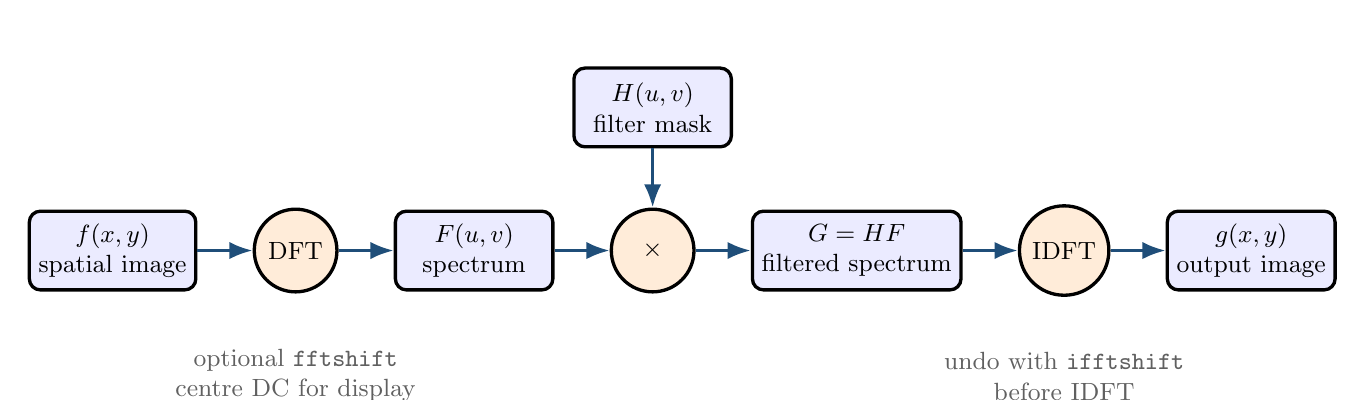
\begin{tikzpicture}[node distance=0.65cm and 0.7cm,>=Latex,font=\small]
  \tikzset{
    data/.style={draw,rounded corners,very thick,fill=blue!8,
      minimum width=2.0cm,minimum height=1.0cm,align=center},
    op/.style={draw,circle,very thick,fill=orange!15,minimum size=1.05cm,align=center}
  }

  \node[data] (f) {$f(x,y)$\\spatial image};
  \node[op,right=of f] (fft) {DFT};
  \node[data,right=of fft] (F) {$F(u,v)$\\spectrum};
  \node[op,right=of F] (mul) {$\times$};
  \node[data,above=0.75cm of mul] (H) {$H(u,v)$\\filter mask};
  \node[data,right=of mul] (G) {$G=HF$\\filtered spectrum};
  \node[op,right=of G] (ifft) {IDFT};
  \node[data,right=of ifft] (g) {$g(x,y)$\\output image};

  \draw[->,very thick,noteBlue] (f) -- (fft);
  \draw[->,very thick,noteBlue] (fft) -- (F);
  \draw[->,very thick,noteBlue] (F) -- (mul);
  \draw[->,very thick,noteBlue] (H) -- (mul);
  \draw[->,very thick,noteBlue] (mul) -- (G);
  \draw[->,very thick,noteBlue] (G) -- (ifft);
  \draw[->,very thick,noteBlue] (ifft) -- (g);

  \node[below=0.58cm of fft,align=center,text=gray!75!black]
    {optional \texttt{fftshift}\\centre DC for display};
  \node[below=0.58cm of ifft,align=center,text=gray!75!black]
    {undo with \texttt{ifftshift}\\before IDFT};
\end{tikzpicture}
}
  \caption{Frequency-domain filtering：把 spectrum 与 transfer function $H(u,v)$ 逐点相乘，再经 IDFT 返回空间域。}
  \label{fig:sc4061-l04-frequency-pipeline}
\end{figure}

完整流程为
\[
  F=\mathcal F\{f\},\qquad
  G=HF,\qquad
  g=\mathcal F^{-1}\{G\}.
\]
$H=1$ 表示完全保留，$H=0$ 表示移除，$0<H<1$ 表示衰减。Low frequency（低频）通常对应 smooth trend、illumination 与大尺度结构；high frequency（高频）通常对应 edge、fine texture 与 abrupt change。不能把 ``低频''直接等同于 signal、``高频''直接等同于 noise：white noise 具有宽频谱，periodic noise 可能只形成少数尖峰，而有效 edges 本身也是高频 signal。

\lecturetopic{SC4061-L04-T05}{Low-pass、High-pass 与 Notch Filtering}

令 centred spectrum 中
\[
  D(u,v)=\sqrt{u^2+v^2}
\]
表示到 DC 的距离。Ideal low-pass filter（理想低通）为
\[
  H_{\mathrm{ILPF}}(u,v)=
  \begin{cases}1,&D(u,v)\le D_0,\\0,&D(u,v)>D_0.\end{cases}
\]
其 sharp cutoff（突变截止）在空间域对应带 sidelobes 的 sinc-like kernel，容易在强边缘产生 ringing artifacts（振铃伪影）。讲义中若写成 $u^2+v^2\le D_0$，当 $D_0$ 表示 radius 时，严格形式应为 $u^2+v^2\le D_0^2$。

Gaussian low-pass filter（高斯低通）平滑衰减：
\[
  \boxed{H_{\mathrm{GLPF}}(u,v)=
  \exp\!\left[-\frac{D^2(u,v)}{2\sigma_f^2}\right]}.
\]
$\sigma_f$ 越大，frequency passband 越宽，图像越清晰；对应 spatial Gaussian kernel 越窄。两个 domains 的宽度成反比，Gaussian 没有 ideal filter 的明显 sidelobes，因此 ringing 更弱。

High-pass filter（高通）可由
\[
  H_{\mathrm{HP}}=1-H_{\mathrm{LP}}
\]
获得，用于提取 edge 与 detail。直接 high-pass 输出主要是细节；sharpening（锐化）通常需要把细节加回原图：$g_{\mathrm{sharp}}=f+\alpha g_{\mathrm{HP}}$。

\begin{figure}[htbp]
  \centering
  \resizebox{0.96\textwidth}{!}{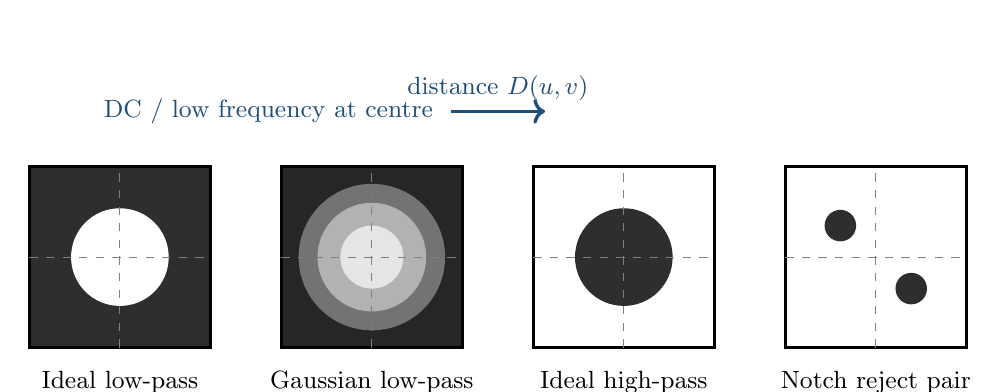
\begin{tikzpicture}[x=1cm,y=1cm,font=\small]
  \tikzset{mask/.style={draw,very thick,minimum width=2.3cm,minimum height=2.3cm}}

  \begin{scope}[shift={(0,0)}]
    \fill[black!82] (0,0) rectangle (2.3,2.3);
    \fill[white] (1.15,1.15) circle (0.62);
    \draw[very thick] (0,0) rectangle (2.3,2.3);
    \draw[dashed,gray] (1.15,0) -- (1.15,2.3);
    \draw[dashed,gray] (0,1.15) -- (2.3,1.15);
    \node[below] at (1.15,-0.18) {Ideal low-pass};
  \end{scope}

  \begin{scope}[shift={(3.2,0)}]
    \fill[black!85] (0,0) rectangle (2.3,2.3);
    \fill[black!55] (1.15,1.15) circle (0.93);
    \fill[black!30] (1.15,1.15) circle (0.69);
    \fill[black!10] (1.15,1.15) circle (0.40);
    \draw[very thick] (0,0) rectangle (2.3,2.3);
    \draw[dashed,gray] (1.15,0) -- (1.15,2.3);
    \draw[dashed,gray] (0,1.15) -- (2.3,1.15);
    \node[below] at (1.15,-0.18) {Gaussian low-pass};
  \end{scope}

  \begin{scope}[shift={(6.4,0)}]
    \fill[white] (0,0) rectangle (2.3,2.3);
    \fill[black!82] (1.15,1.15) circle (0.62);
    \draw[very thick] (0,0) rectangle (2.3,2.3);
    \draw[dashed,gray] (1.15,0) -- (1.15,2.3);
    \draw[dashed,gray] (0,1.15) -- (2.3,1.15);
    \node[below] at (1.15,-0.18) {Ideal high-pass};
  \end{scope}

  \begin{scope}[shift={(9.6,0)}]
    \fill[white] (0,0) rectangle (2.3,2.3);
    \fill[black!82] (0.70,1.55) circle (0.20);
    \fill[black!82] (1.60,0.75) circle (0.20);
    \draw[very thick] (0,0) rectangle (2.3,2.3);
    \draw[dashed,gray] (1.15,0) -- (1.15,2.3);
    \draw[dashed,gray] (0,1.15) -- (2.3,1.15);
    \node[below] at (1.15,-0.18) {Notch reject pair};
  \end{scope}

  \draw[->,very thick,noteBlue] (5.35,3.0) -- (6.55,3.0)
    node[midway,above] {distance $D(u,v)$};
  \node[anchor=east,text=noteBlue] at (5.25,3.0) {DC / low frequency at centre};
\end{tikzpicture}
}
  \caption{以 centred spectrum 表示的常见 masks。白色表示 pass，黑色表示 reject；notch pair 同时抑制实值图像中共轭对称的周期噪声峰。}
  \label{fig:sc4061-l04-filter-masks}
\end{figure}

Notch reject filter（陷波滤波器）只抑制特定 frequencies，适合 spectrum 中呈 conjugate peak pair（共轭峰对）的 sinusoidal interference。Band-reject filter（带阻滤波器）删除一段 frequency band；若干扰只占少数尖峰，notch 往往比删除整个 band 更能保留图像信息。

\textbf{对应例题：}
\begin{itemize}
  \item \relatedexercise{SC4061-L04-E02}{Gaussian Low-pass 的 $\sigma_f$}；
  \item \relatedexercise{SC4061-L04-E03}{Periodic Noise 与 Notch Pair}。
\end{itemize}

\lecturetopic{SC4061-L04-T06}{何时 Fourier Basis 会简化问题}

Fourier modes 可在不指定算符时作为一组 periodic orthogonal basis（周期正交基）定义；$u,v$ 首先只是 mode labels。它们是 cyclic translations（循环平移）的共同 eigenvectors，也使所有 periodic linear shift-invariant operators（周期线性平移不变算符），包括 circular convolution，变为 diagonal。不同 operators 共享 eigenvectors，但 eigenvalues 不同：shift 的 eigenvalue 为 $e^{-j2\pi u/M}$，convolution 的 eigenvalue 为 kernel spectrum $H(u,v)$。

并非所有 operators 都被 Fourier transform 简化。例如 spatially varying pointwise multiplication（空间变化的逐点乘法）
\[
  g(x,y)=m(x,y)f(x,y)
\]
在 pixel basis 中已经 diagonal，而在 frequency domain 中变成 convolution $G=M*F$，会混合多个 modes。应选择使目标 operator diagonal 或 sparse 的 domain：小型 local/spatially varying 操作常在 spatial domain 更自然；large shift-invariant convolution、global periodic interference 与 frequency-selective filtering 常在 frequency domain 更自然。

\subsection{MATLAB 速查}

附件代码的核心对应关系为
\begin{verbatim}
F = fftshift(fft2(f));
G = H .* F;
g = real(ifft2(ifftshift(G)));
imagesc(log1p(abs(F)));
\end{verbatim}
直接保留 centred spectrum 的一个矩形区域相当于 crude ideal low-pass（粗糙理想低通），可能产生方向偏置与 ringing；更平滑的 Gaussian mask 通常更稳健。

\subsection{一分钟回顾}

DFT 用 $MN$ 个二维 complex exponential modes 表示 $M\times N$ image；magnitude 表示 mode 强度，phase 保存空间位置，\texttt{fftshift} 只改变排列。FFT 高效计算 DFT，convolution theorem 使 shift-invariant convolution 变成 spectrum multiplication，但小 kernel 与 spatially varying operator 不一定适合 FFT。Low-pass 保留趋势、high-pass 保留细节，Gaussian cutoff 比 ideal cutoff 更少 ringing；periodic noise 常以共轭尖峰出现，应成对使用 notch reject。

% Actual class: 05
% Slide decks: L3 (full) Frequency slides; L4 (full) Edge slides
% Exact scope: L3 pp. 32--45 (Part 3); L4 pp. 1--19 (Part 1)
% NTULearn supplement: transcripts 58735 and 58959
% Human verified: Yes

\section{第 05 节课：Frequency Extensions and Edge Detection}
\label{lecture:SC4061-L05}

\lecturemeta
  {SC4061-L05}
  {2026-09-08}
  {L3 (full) Frequency slides；L4 (full) Edge slides}
  {L3 pp.~32--45（Part 3，其中 p.~32 为 quiz 收尾）；L4 pp.~1--19（Part 1）}
  {课程视频 L3 Part 3 与 L4 Part 1（字幕 58735、58959 核对）}
  {已确认（2026-09-08）}

\subsection{本讲主线}

Fourier transform（傅里叶变换）提供 global frequency representation（全局频率表示），但 localized discontinuity（局部不连续）可能激活大量 Fourier coefficients（傅里叶系数）；wavelet transform（小波变换）则同时保留 frequency/scale（频率/尺度）和 approximate location（近似位置）。课程随后从 image enhancement（图像增强）转向 feature extraction（特征提取）：先用 first/second derivatives（一阶/二阶导数）描述 intensity change（强度变化），再由 Sobel、LoG 和 Canny 把变化转为 binary edge map（二值边缘图）。

\lecturetopic{SC4061-L05-T01}{Dense Fourier Spectrum 与 Wavelet Localization}

任意 $M\times N$ image 都可展开为 global Fourier modes：
\[
  f(x,y)=\frac{1}{MN}\sum_{u=0}^{M-1}\sum_{v=0}^{N-1}
  F(u,v)e^{j2\pi(ux/M+vy/N)}.
\]
一个 piecewise-constant silhouette（分段常数轮廓）在 spatial domain 可能很简单，但 sharp boundary（尖锐边界）不能由少数平滑、全局支撑的 sinusoids 精确表示，因此 spectrum 往往是 dense（稠密）的。讲义 p.~32 的 ``no zeros'' 应理解为这一典型趋势，不是保证每个 coefficient 都严格非零的定理。

\begin{figure}[htbp]
  \centering
  \resizebox{0.95\textwidth}{!}{\begin{tikzpicture}[x=0.9cm,y=0.78cm,font=\small,>=Latex]
  \tikzset{
    axis/.style={->,semithick,gray!75!black},
    signal/.style={very thick,noteBlue},
    basis/.style={thick,orange!85!black},
    support/.style={fill=blue!7,draw=none}
  }

  \begin{scope}[shift={(0,0)}]
    \node[font=\bfseries] at (3.1,3.25) {Fourier basis（全局支撑）};
    \draw[axis] (0,0) -- (6.2,0) node[right] {$x$};
    \draw[axis] (0,0) -- (0,2.6) node[above] {value};
    \draw[signal] (0.2,0.35) -- (2.85,0.35) -- (2.85,2.15) -- (5.95,2.15);
    \draw[basis,samples=80,domain=0.2:5.95]
      plot (\x,{1.25+0.28*sin(180*\x)});
    \draw[basis,dashed,samples=80,domain=0.2:5.95]
      plot (\x,{1.25+0.18*sin(360*\x)});
    \draw[densely dotted,gray!70] (2.85,0) -- (2.85,2.55);
    \node[align=center,text=gray!75!black] at (3.1,-0.7)
      {local discontinuity activates\\many global coefficients};
  \end{scope}

  \begin{scope}[shift={(8.0,0)}]
    \node[font=\bfseries] at (3.1,3.25) {Wavelet basis（局部支撑）};
    \draw[axis] (0,0) -- (6.2,0) node[right] {$x$};
    \draw[axis] (0,0) -- (0,2.6) node[above] {value};
    \path[support] (2.0,0.05) rectangle (3.75,2.5);
    \draw[signal] (0.2,0.35) -- (2.85,0.35) -- (2.85,2.15) -- (5.95,2.15);
    \draw[basis] (1.95,1.25)
      .. controls (2.2,1.25) and (2.25,2.25) .. (2.7,2.25)
      .. controls (3.15,2.25) and (3.2,0.25) .. (3.65,0.25)
      .. controls (3.9,0.25) and (3.95,1.25) .. (4.2,1.25);
    \draw[densely dotted,gray!70] (2.85,0) -- (2.85,2.55);
    \node[align=center,text=gray!75!black] at (3.1,-0.7)
      {coefficient carries\\scale/frequency and location};
  \end{scope}
\end{tikzpicture}
}
  \caption{Fourier basis 是 global support（全局支撑）；localized wavelet basis 可把 coefficient 与发生位置及尺度联系起来。}
  \label{fig:sc4061-l05-fourier-wavelet}
\end{figure}

Wavelet decomposition（小波分解）通常产生 $LL$ approximation（低频近似）以及 $LH,HL,HH$ directional details（方向细节）。它适合同时需要 spatial localization 和 multi-scale frequency information（多尺度频率信息）的 edges 与 textures；但不能据此断言 wavelet 在所有任务上都优于 Fourier。Global periodic structure（全局周期结构）与 shift-invariant convolution（平移不变卷积）仍常在 Fourier domain 更自然。

\textbf{对应例题：}
\relatedexercise{SC4061-L05-E01}{Local Edge 的 Fourier/Wavelet Representation}。

\lecturetopic{SC4061-L05-T02}{U-Net、Up-sampling 与 Global Modeling}

U-Net 的 encoder（编码器）通过 down-sampling 建立 large receptive field（大感受野）与 multi-scale representation；decoder（解码器）再 up-sample 为 dense output（稠密输出）。Down-sampling 是 many-to-one mapping，会丢失 high-frequency detail，因此普通 interpolation 不能真正恢复被删除的信息；learned decoder 只能依据 training prior（训练先验）估计细节。Skip connections（跳跃连接）把 encoder 中的 high-resolution features 送给 decoder，用来补回定位信息。

\begin{figure}[htbp]
  \centering
  \resizebox{0.92\textwidth}{!}{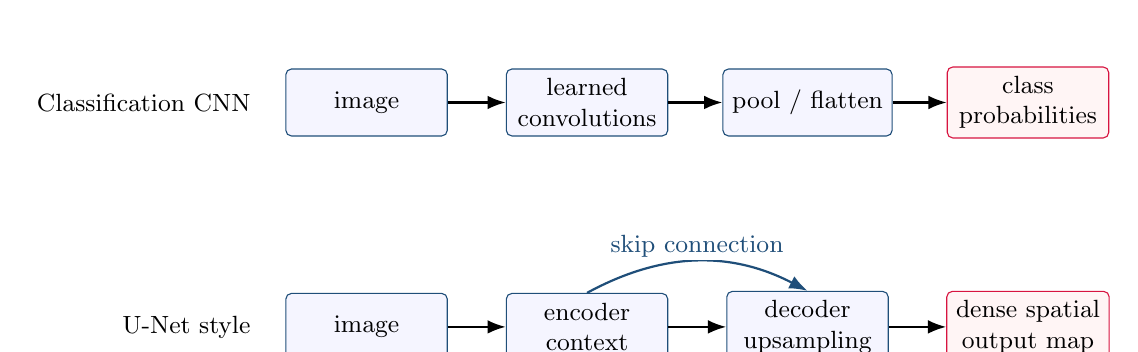
\begin{tikzpicture}[
  >=Latex,
  stage/.style={draw=noteBlue, rounded corners=2pt, minimum width=2.05cm,
    minimum height=0.85cm, align=center, fill=blue!4},
  dense/.style={draw=ntuRed, rounded corners=2pt, minimum width=2.05cm,
    minimum height=0.85cm, align=center, fill=red!4},
  every node/.style={font=\small}
]
  \node[stage] (im1) at (0,1.6) {image};
  \node[stage] (conv1) at (2.8,1.6) {learned\\convolutions};
  \node[stage] (pool1) at (5.6,1.6) {pool / flatten};
  \node[dense] (class) at (8.4,1.6) {class\\probabilities};
  \draw[->,thick] (im1)--(conv1);
  \draw[->,thick] (conv1)--(pool1);
  \draw[->,thick] (pool1)--(class);
  \node[anchor=east] at (-1.35,1.6) {Classification CNN};

  \node[stage] (im2) at (0,-1.25) {image};
  \node[stage] (enc) at (2.8,-1.25) {encoder\\context};
  \node[stage] (dec) at (5.6,-1.25) {decoder\\upsampling};
  \node[dense] (map) at (8.4,-1.25) {dense spatial\\output map};
  \draw[->,thick] (im2)--(enc);
  \draw[->,thick] (enc)--(dec);
  \draw[->,thick] (dec)--(map);
  \draw[->,thick,noteBlue,bend left=28] (enc.north) to
    node[above,fill=white,inner sep=1pt] {skip connection} (dec.north);
  \node[anchor=east] at (-1.35,-1.25) {U-Net style};
\end{tikzpicture}
}
  \caption{Classification CNN 与 U-Net-style dense prediction。Skip connection 缓解 down-sampling 带来的 localization loss。}
  \label{fig:sc4061-l05-unet}
\end{figure}

课程引用 Deep Fourier Up-Sampling 说明一种思路：spatial interpolation 与 transposed convolution 主要依赖 local neighbourhood，而 Fourier coefficients 控制 global modes。由 convolution theorem，
\[
  g=f*h
  \quad\Longleftrightarrow\quad
  G(u,v)=F(u,v)H(u,v),
\]
frequency-domain operation 能直接建模全局依赖。不过 changing resolution（改变分辨率）不能等同于随意拉伸 spectrum；DFT grid、normalization、periodicity 与 conjugate symmetry 都必须保持一致。Fourier up-sampling 在特定 datasets 上的 PSNR/SSIM 提升是 empirical evidence（实验证据），不是对所有任务有效的普遍保证。

\lecturetopic{SC4061-L05-T03}{Fourier/Wavelet into Deep Learning 的研究逻辑}

本段扩展阅读的重点不是记住论文 architecture，而是理解四步 research workflow：
\begin{enumerate}
  \item \textbf{Intuition：}指出 local up-sampling 难以利用 global dependency；
  \item \textbf{Result：}实现 periodic padding、area/corner interpolation 等候选方案并比较；
  \item \textbf{Scientific explanation：}分析 resolution change 与 Fourier coefficients 的严格关系，排除偶然提升；
  \item \textbf{Extension：}若 Fourier 缺乏 localization，引入 Haar wavelet 等同时保存低频结构与高频细节。
\end{enumerate}
Wavelet-based down/up-sampling 可把 approximation 与 directional details 分开处理，并在 reconstruction 时重新组合。它为 edges 和 fine structures 提供合适的 inductive bias（归纳偏置），但最终优劣仍需由任务、数据、metric 与 ablation study（消融实验）验证。

\lecturetopic{SC4061-L05-T04}{Image Edges、Gradient 与 Curvature}

Edge（边缘）是一串相互连接的 edgels（边缘元素），通常对应 image intensity 的快速变化。它可能来自 object/depth/material boundary，也可能来自 illumination、texture 或 noise，因此 ``detected edge'' 不必然等于真实 object boundary。

沿垂直于 edge 的方向观察 smooth step profile：edge centre 附近 first derivative 的 magnitude 最大，而 second derivative 改变符号并经过 zero crossing。这里的 curvature 指 intensity profile 的二阶导数，不是边界曲线的 geometric curvature。

\begin{figure}[htbp]
  \centering
  \resizebox{0.98\textwidth}{!}{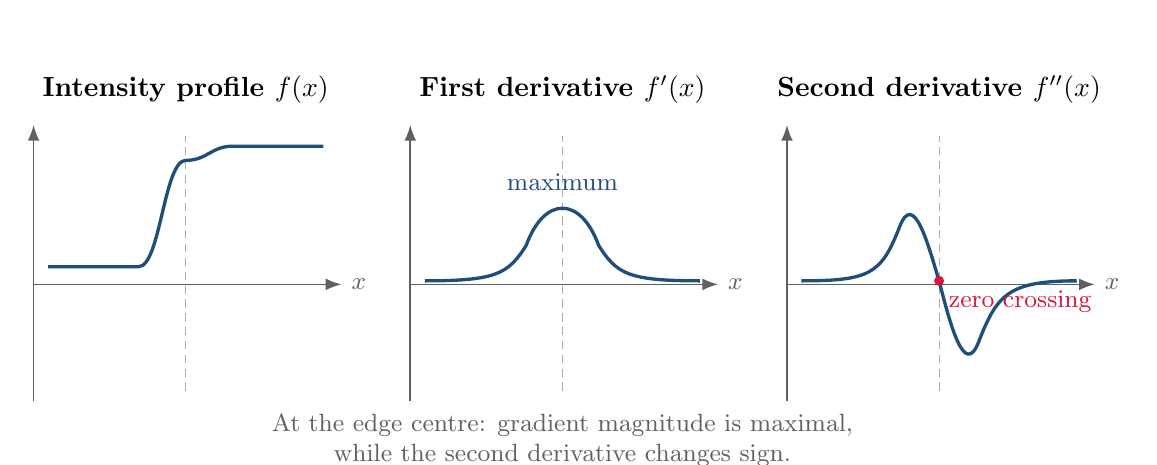
\begin{tikzpicture}[x=0.92cm,y=0.9cm,font=\small,>=Latex]
  \tikzset{
    axis/.style={->,semithick,gray!75!black},
    signal/.style={very thick,noteBlue},
    guide/.style={densely dashed,gray!65}
  }

  \foreach \xshift/\title in {0/{Intensity profile $f(x)$},5.2/{First derivative $f'(x)$},10.4/{Second derivative $f''(x)$}} {
    \begin{scope}[shift={(\xshift,0)}]
      \node[font=\bfseries] at (2.1,2.75) {\title};
      \draw[axis] (0,0) -- (4.25,0) node[right] {$x$};
      \draw[axis] (0,-1.65) -- (0,2.25);
      \draw[guide] (2.1,-1.5) -- (2.1,2.1);
    \end{scope}
  }

  \begin{scope}[shift={(0,0)}]
    \draw[signal] (0.2,0.25) -- (1.45,0.25)
      .. controls (1.75,0.25) and (1.8,1.75) .. (2.1,1.75)
      .. controls (2.4,1.75) and (2.45,1.95) .. (2.75,1.95)
      -- (4.0,1.95);
  \end{scope}

  \begin{scope}[shift={(5.2,0)}]
    \draw[signal] (0.2,0.05)
      .. controls (1.2,0.05) and (1.35,0.15) .. (1.6,0.55)
      .. controls (1.85,1.25) and (2.35,1.25) .. (2.6,0.55)
      .. controls (2.85,0.15) and (3.0,0.05) .. (4.0,0.05);
    \node[above,text=noteBlue] at (2.1,1.18) {maximum};
  \end{scope}

  \begin{scope}[shift={(10.4,0)}]
    \draw[signal] (0.2,0.05)
      .. controls (1.15,0.05) and (1.3,0.15) .. (1.55,0.8)
      .. controls (1.75,1.35) and (1.95,0.55) .. (2.1,0.05)
      .. controls (2.25,-0.55) and (2.45,-1.35) .. (2.65,-0.8)
      .. controls (2.9,-0.15) and (3.05,0.05) .. (4.0,0.05);
    \fill[ntuRed] (2.1,0.05) circle (1.8pt);
    \node[below right,text=ntuRed] at (2.1,0.05) {zero crossing};
  \end{scope}

  \node[align=center,text=gray!75!black] at (7.3,-2.2)
    {At the edge centre: gradient magnitude is maximal,\\
     while the second derivative changes sign.};
\end{tikzpicture}
}
  \caption{平滑 step edge 的 intensity、first derivative 与 second derivative。Gradient peak 和 LoG zero crossing 提供两种定位方式。}
  \label{fig:sc4061-l05-edge-profiles}
\end{figure}

二维 gradient 为
\[
  \nabla f=\begin{bmatrix}G_x\\G_y\end{bmatrix},\qquad
  M=\sqrt{G_x^2+G_y^2},\qquad
  \alpha=\operatorname{atan2}(G_y,G_x).
\]
$\alpha$ 是 intensity 增长最快的 gradient direction，与 edge tangent direction（边缘切向）垂直。Edge processing 的完整流程为 edge filtering $\rightarrow$ edgel detection $\rightarrow$ edgel linking；本节只到前两步，linking 留待下一讲。

\lecturetopic{SC4061-L05-T05}{Prewitt 与 Sobel Gradient Filters}

讲义采用的 Sobel kernels 可写为
\[
  K_x=\begin{bmatrix}-1&0&1\\-2&0&2\\-1&0&1\end{bmatrix},\qquad
  K_y=\begin{bmatrix}-1&-2&-1\\0&0&0\\1&2&1\end{bmatrix}.
\]
$K_x$ 计算 $x$ 方向的 intensity change，因而响应 vertical edge；$K_y$ 响应 horizontal edge。整体改变 kernel sign 只会把 gradient direction 旋转 $180^\circ$，不改变 magnitude 或 edge location。

Sobel 可分解为 central difference 与正交方向的 $[1,2,1]$ smoothing，因而比单纯两像素差分稳定。常用快速幅值近似为
\[
  \sqrt{G_x^2+G_y^2}\approx |G_x|+|G_y|.
\]
它仍有 noise sensitivity、response strength 不一以及 broad/thick edge response 三个问题。

\textbf{对应例题：}
\relatedexercise{SC4061-L05-E02}{Sobel Gradient 与 Edge Direction}。

\lecturetopic{SC4061-L05-T06}{Laplacian of Gaussian 与 Zero Crossing}

Laplacian（二阶拉普拉斯算子）为
\[
  \nabla^2 f=\frac{\partial^2f}{\partial x^2}+\frac{\partial^2f}{\partial y^2}.
\]
直接求 second derivative 会放大 noise，因此 LoG 先以 Gaussian $G_\sigma$ smoothing，再求 Laplacian。利用 differentiation 与 convolution 的可交换性，
\[
  \boxed{f*(\nabla^2G_\sigma)=\nabla^2(f*G_\sigma)}.
\]
所以可预先构造一个 LoG kernel，一次 convolution 后从 sign change 中寻找 zero crossing。一个理想 step edge 会产生一正一负的 double-lobe response，二者之间的 zero crossing 对应 edge centre。增大 $\sigma$ 会加强 smoothing 并偏向较粗尺度的 edges，但也降低 localization precision。

LoG 比裸 Laplacian 更抗噪，却不代表 ``不受噪声影响''：残余 noise 仍可能因二阶导数被放大，而且 zero-crossing map 可能产生多余轮廓。

\textbf{对应例题：}
\relatedexercise{SC4061-L05-E03}{LoG 的 Smoothing 与 Zero Crossing}。

\lecturetopic{SC4061-L05-T07}{Canny Edge Detector}

Canny 重新采用 first-derivative route，并逐项处理 Sobel 的三个问题：
\begin{enumerate}
  \item \textbf{Derivative of Gaussian (DoG)：}以 $\partial G_\sigma/\partial x$、$\partial G_\sigma/\partial y$ 得到 $G_x,G_y$，把 smoothing 与 differentiation 合并；
  \item \textbf{Non-maximum suppression (NMS)：}沿 gradient direction 比较 $M(x,y)$，仅保留 local maximum，把宽 ridge 压成近似 single-pixel-wide path；
  \item \textbf{Hysteresis thresholding：}使用 $t_L<t_H$。$M\ge t_H$ 为 strong edge，$M<t_L$ 删除；中间的 weak edge 仅在与 strong edge 连通时保留。
\end{enumerate}

\begin{figure}[htbp]
  \centering
  \resizebox{0.98\textwidth}{!}{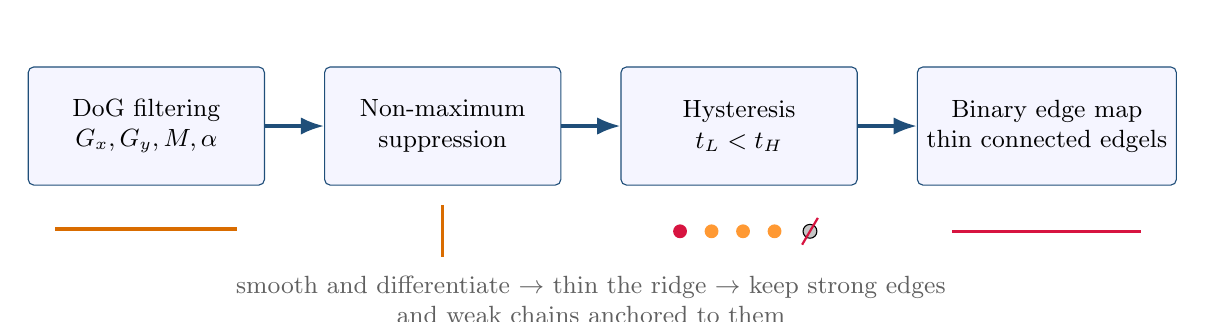
\begin{tikzpicture}[font=\small,>=Latex,node distance=0.6cm and 0.75cm]
  \tikzset{
    stage/.style={draw=noteBlue,rounded corners=2pt,minimum width=3.0cm,
      minimum height=1.5cm,align=center,fill=blue!4},
    arrow/.style={->,very thick,noteBlue}
  }

  \node[stage] (dog) {DoG filtering\\$G_x,G_y,M,\alpha$};
  \node[stage,right=of dog] (nms) {Non-maximum\\suppression};
  \node[stage,right=of nms] (hys) {Hysteresis\\$t_L<t_H$};
  \node[stage,right=of hys] (map) {Binary edge map\\thin connected edgels};
  \draw[arrow] (dog) -- (nms);
  \draw[arrow] (nms) -- (hys);
  \draw[arrow] (hys) -- (map);

  \draw[very thick,orange!85!black] ($(dog.south west)+(0.35,-0.55)$)
    .. controls +(0.7,0) and +(-0.7,0) .. ($(dog.south east)+(-0.35,-0.55)$);
  \draw[very thick,orange!85!black] ($(nms.south)+(0,-0.9)$) -- ($(nms.south)+(0,-0.25)$);

  \foreach \dx/\dotcolor in {-0.75/ntuRed,-0.35/orange!80,0.05/orange!80,0.45/orange!80} {
    \fill[\dotcolor] ($(hys.south)+(\dx,-0.58)$) circle (2.5pt);
  }
  \draw[fill=gray!45] ($(hys.south)+(0.9,-0.58)$) circle (2.5pt);
  \draw[ntuRed,thick] ($(hys.south)+(0.8,-0.75)$) -- ($(hys.south)+(1.0,-0.41)$);

  \draw[very thick,ntuRed] ($(map.south west)+(0.45,-0.58)$) -- ($(map.south east)+(-0.45,-0.58)$);
  \node[align=center,text=gray!75!black] at ($(nms.south)!0.5!(hys.south)+(0,-1.45)$)
    {smooth and differentiate $\rightarrow$ thin the ridge $\rightarrow$ keep strong edges\\
     and weak chains anchored to them};
\end{tikzpicture}
}
  \caption{Canny pipeline：DoG 抑制噪声，NMS 处理厚度，双阈值 hysteresis 处理强度变化。}
  \label{fig:sc4061-l05-canny}
\end{figure}

NMS 必须沿 gradient direction 扫描，因为该方向横穿 edge；edge 延伸方向与之垂直。Hysteresis 的 connectivity 可沿 weak-edge chain 传播，只要整条链最终 anchored to a strong edge。实际使用至少需要选择 Gaussian scale/kernel support 以及 $t_L,t_H$；更强 smoothing 可减少 noise，却可能合并近邻 edges 或损失精确位置。

Canny 能检测任意 orientation，包括 $30^\circ$ edge，因为 $G_x,G_y$ 合成连续方向的 gradient vector，而不是只保留水平/竖直二选一。输出仍可能有 broken edges 或不完整的 global shape；这些问题将由下一讲 edge linking 与 Hough transform 处理。

\textbf{对应例题：}
\relatedexercise{SC4061-L05-E04}{Hysteresis Thresholding 的 Strong/Weak Edges}。

\subsection{一分钟回顾}

Fourier representation 是 global 的，局部 sharp edge 可能产生 dense spectrum；wavelet 以 localized multi-scale basis 补充位置信息。U-Net 的 down/up-sampling 存在信息丢失，skip connection 与 frequency/wavelet modules 分别提供定位和全局/多尺度建模。Edge 可由 first-derivative peak 或 second-derivative zero crossing 描述；Sobel 简单但会产生噪声、强度和厚度问题。LoG 在 smoothing 后检测 zero crossing；Canny 依次用 DoG、NMS 与 hysteresis 得到细而连贯的 binary edge map。

% Actual class: 06
% Slide deck: L4 (full) Edge slides
% Exact scope: L4 pp. 20--40 (Parts 2--3)
% NTULearn supplement: transcripts 58958 and 58957
% Human verified: Yes

\section{第 06 节课：Edge Linking and Deep Edge}
\label{lecture:SC4061-L06}

\lecturemeta
  {SC4061-L06}
  {2026-09-15}
  {L4 (full) Edge slides}
  {L4 pp.~20--40（Part 2 与 Part 3）}
  {课程视频 Edge Part 2 与 Part 3（字幕 58958、58957 核对）}
  {已确认（2026-09-15）}

\subsection{本讲主线}

Canny 等 detector 最终只对单个 pixel 判断是否为 edgel（边缘元素）；edge linking（边缘连接）还要从全局判断哪些 edgels 属于同一条 edge。Hough transform（霍夫变换）把这种全局组合问题改写为 parameter-space voting（参数空间投票）。课程随后以 Harris、SIFT 和 RCF 为扩展阅读，说明视觉表示从 edge 走向 corner、feature point，再走向由 CNN 学习 multi-level、multi-scale edge features。

\lecturetopic{SC4061-L06-T01}{Edgel Linking 与 Hough Line Geometry}

Thresholding 后得到 binary map $E(x,y)\in\{0,1\}$；其中的 $1$ 只表示一个 edgel，并未给出完整 edge、所属分组或全局方程。此前 Sobel、LoG、Canny 主要依赖 local neighbourhood，而 linking 必须利用相距较远像素之间的共线或共曲线关系。

令直线的单位法向量为
\[
  \mathbf n=(\cos\theta,\sin\theta)^{\mathsf T}.
\]
原点到直线的 signed distance（带符号距离）为 $\rho$，则直线上任一点 $\mathbf p=(x,y)^{\mathsf T}$ 满足
\[
  \boxed{\mathbf n^{\mathsf T}\mathbf p=\rho}
  \qquad\Longleftrightarrow\qquad
  \boxed{x\cos\theta+y\sin\theta=\rho}.
\]
Normal form（法线式）对 vertical line 也保持有限参数；相比之下 $y=ax+b$ 无法以有限 slope $a$ 表示竖直线。严格地说，参数具有
\[
  (\rho,\theta)\sim(-\rho,\theta+\pi)
\]
的冗余；只有规定例如 $\theta\in[-\pi/2,\pi/2)$ 且允许 signed $\rho$ 后，才可把一对参数视为唯一的直线。

\lecturetopic{SC4061-L06-T02}{Image--Hough Duality、Voting 与 Generalization}

同一方程有两种互补解释：固定 $(\rho,\theta)$，变化的 $(x,y)$ 在 image space 中组成一条直线；固定 edgel $(x_p,y_p)$，变化的参数满足
\[
  \rho(\theta)=x_p\cos\theta+y_p\sin\theta,
\]
在 Hough space 中形成一条 sinusoid（正弦曲线）。因此一个 edgel ``给所有经过它的直线投票''，等价于沿该 sinusoid 给离散 accumulator $A(\rho,\theta)$ 加一。共线 edgels 的 curves 在同一 $(\rho^*,\theta^*)$ 附近相交并形成 peak。

\begin{figure}[htbp]
  \centering
  \resizebox{0.94\textwidth}{!}{\begin{tikzpicture}[font=\small,>=Latex]
  \begin{scope}[xshift=0cm]
    \draw[->,thick] (-0.3,0) -- (3.4,0) node[right] {$x$};
    \draw[->,thick] (0,-1.3) -- (0,1.7) node[above] {$y$};
    \draw[very thick,noteBlue] (1,-1.15) -- (1,1.45);
    \foreach \yy/\cc in {-0.7/ntuRed,0/orange!85!black,0.7/teal!75!black} {
      \fill[\cc] (1,\yy) circle (3.2pt);
    }
    \node[align=center] at (1.65,-1.55) {image space\\共线 edgels};
  \end{scope}

  \draw[->,very thick,gray!65] (3.7,0.2) -- (5.1,0.2)
    node[midway,above,align=center] {vote};

  \begin{scope}[xshift=5.7cm,x=0.035cm,y=1.05cm]
    \draw[->,thick] (-85,0) -- (88,0) node[right] {$\theta$};
    \draw[->,thick] (0,-1.35) -- (0,1.7) node[above] {$\rho$};
    \draw[ntuRed,very thick,samples=90,domain=-80:80,smooth]
      plot (\x,{cos(\x)-0.7*sin(\x)});
    \draw[orange!85!black,very thick,samples=90,domain=-80:80,smooth]
      plot (\x,{cos(\x)});
    \draw[teal!75!black,very thick,samples=90,domain=-80:80,smooth]
      plot (\x,{cos(\x)+0.7*sin(\x)});
    \fill[noteBlue] (0,1) circle (3.5pt);
    \draw[dashed,noteBlue] (0,0) -- (0,1);
    \node[anchor=west,noteBlue] at (5,1.18) {peak $(\theta^*,\rho^*)$};
    \node[align=center] at (0,-1.65) {Hough space\\sinusoids intersect};
  \end{scope}
\end{tikzpicture}
}
  \caption{Image--Hough duality：image space 中同一直线上的多个 edgels，在 Hough space 中投票给共同的 parameter peak。}
  \label{fig:sc4061-l06-hough-voting}
\end{figure}

实际算法把 $\theta$ 与 $\rho$ 量化为 bins。过粗会合并邻近直线；过细会把同一 noisy edge 的票分散到邻近 bins，并增加内存与计算量。Peak 给出的是 infinite line；若要得到 finite segment，还需沿该直线寻找 supporting edgels，并用 gap tolerance 决定端点。高票通常意味着有更多共线支持，但不必然严格等于最长线，还受 edge thickness、sampling density、quantization 与 thresholding 影响。

\textbf{对应例题：}
\begin{itemize}
  \item \relatedexercise{SC4061-L06-E01}{单点 Hough Curve 与共线投票}；
  \item \relatedexercise{SC4061-L06-E02}{Hough 参数特殊情形 Quiz}。
\end{itemize}

Hough transform 可推广到任意 parameterized curve
\[
  F(x,y;\boldsymbol\phi)=0.
\]
例如圆需要 $\boldsymbol\phi=(a,b,r)$，accumulator 由二维变为三维。若第 $j$ 个参数离散为 $B_j$ 个 bins，存储规模为 $\prod_j B_j$；因此参数维数增加会迅速带来 computational cost，而不只是增加一个简单循环。

\lecturetopic{SC4061-L06-T03}{Feature Points、RCF 与 Vision Levels}

Extended reading 从 edge 扩展到 Harris corner，再到 SIFT keypoint：corner 在两个独立方向上都有明显 intensity change；更一般的 feature point 只要求局部结构 distinctive（可区分），并可追求 scale/rotation robustness。讲义并未展开二者的完整算法，重点是说明 edge 只是视觉特征的一种。

RCF（Richer Convolutional Features for Edge Detection）以 VGG-16 的多个 convolution stages 产生 side outputs。Shallow layers 保留高分辨率与精确定位，却容易响应 texture/noise；deep layers 具有更大 receptive field 和更强 semantic context，却较粗糙。RCF 将不同层的 edge evidence resize 后融合，实现 image-to-image dense prediction。讲义引用论文在 BSDS500 上报告 ODS F-measure $0.811$（8 FPS）及 fast version $0.806$（30 FPS）；这些是原论文实验结果，不是本课程重新验证的普遍保证。

\begin{figure}[htbp]
  \centering
  \resizebox{0.94\textwidth}{!}{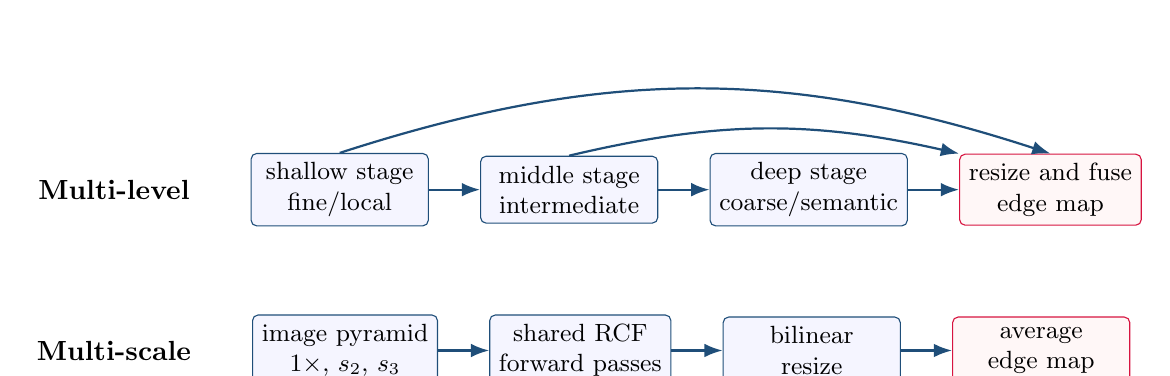
\begin{tikzpicture}[font=\small,>=Latex,node distance=0.55cm and 0.65cm]
  \tikzset{
    box/.style={draw=noteBlue,rounded corners=2pt,minimum width=2.25cm,
      minimum height=0.85cm,align=center,fill=blue!4},
    fusion/.style={draw=ntuRed,rounded corners=2pt,minimum width=2.25cm,
      minimum height=0.85cm,align=center,fill=red!3},
    arrow/.style={->,thick,noteBlue}
  }

  \node[font=\bfseries,anchor=east] (mlabel) {Multi-level};
  \node[box,right=of mlabel] (s1) {shallow stage\\fine/local};
  \node[box,right=of s1] (s3) {middle stage\\intermediate};
  \node[box,right=of s3] (s5) {deep stage\\coarse/semantic};
  \node[fusion,right=of s5] (fuse) {resize and fuse\\edge map};
  \draw[arrow] (s1) -- (s3);
  \draw[arrow] (s3) -- (s5);
  \draw[arrow] (s1.north) to[bend left=18] (fuse.north);
  \draw[arrow] (s3.north) to[bend left=13] (fuse.north west);
  \draw[arrow] (s5) -- (fuse);

  \node[font=\bfseries,anchor=east,below=1.55cm of mlabel] (slabel) {Multi-scale};
  \node[box,right=of slabel] (pyr) {image pyramid\\$1\times,\,s_2,\,s_3$};
  \node[box,right=of pyr] (rcf) {shared RCF\\forward passes};
  \node[box,right=of rcf] (resize) {bilinear\\resize};
  \node[fusion,right=of resize] (avg) {average\\edge map};
  \draw[arrow] (pyr) -- (rcf);
  \draw[arrow] (rcf) -- (resize);
  \draw[arrow] (resize) -- (avg);
\end{tikzpicture}
}
  \caption{RCF 中两种互补的信息融合：multi-level 来自不同网络深度，multi-scale 来自不同输入尺寸。}
  \label{fig:sc4061-l06-rcf-fusion}
\end{figure}

\begin{center}
\begin{tabular}{lll}
  \toprule
  概念 & 改变的对象 & 主要作用 \\
  \midrule
  Multi-level & 同一次 network 中不同深度的 feature maps & 结合定位细节与语义上下文 \\
  Multi-scale & 不同尺寸的 input images & 适应不同大小的结构 \\
  \bottomrule
\end{tabular}
\end{center}

Multi-scale pipeline 先构建 image pyramid，对每个尺度分别执行 RCF，再以 bilinear interpolation 恢复到原尺寸并 average。课程前半段的层次可概括为 low-level：image $\to$ image；middle-level：image $\to$ feature；high-level：image/features $\to$ decision。边界不是绝对的，例如 edge map 形式上仍是 image，但作为下游输入时通常视为 middle-level feature。智能测量与缺陷检测中，高质量 low/middle-level output 本身也可能是最终目标。

\subsection{一分钟回顾}

Edge detector 产生 edgels，Hough transform 再用 global voting 恢复参数化 edge。一个 image point 对应 Hough sinusoid，多个共线点共享 accumulator peak；$\theta$ 描述 normal direction 而非 edge tangent。RCF 以 shallow/deep feature fusion 实现 multi-level edge detection，再以 image pyramid 引入 multi-scale information。有效研究迭代应由结果分析指导修改，而不是只做 random trial。

% Actual class: 07
% Source: LEC05 Image Segmentation - 2026, PDF pp. 1--26
% Video scope: transcripts 60715 (Introduction) and 60722 (Thresholding)
% This is the agreed study split, not a teacher-labelled video/week mapping.

\section{第 07 节课：Image Segmentation and Thresholding}
\label{lecture:SC4061-L07}

\lecturemeta
  {SC4061-L07}
  {2026-09-22}
  {LEC05 Image Segmentation -- 2026}
  {本次学习 pp.~1--26：Introduction 与 Thresholding}
  {字幕 60715、60722；后两个视频的 Texture / Semantic Segmentation 暂未纳入}
  {已确认本次学习范围（2026-09-22）}

\subsection{本讲主线}

Edge detection 寻找图像中变化明显的位置；image segmentation（图像分割）把像素划分到不同区域。本讲先用灰度直方图描述区域，再用 Otsu 自动选择全局阈值，最后用 Niblack 的局部阈值处理不均匀照明。本次按前两个视频组织学习，后续内容另记。

\lecturetopic{SC4061-L07-T01}{从边缘到区域：分割的输出与依据}

分割可以表示为 label map（标签图）$L(x,y)$：每个像素获得一个区域标签；二类分割也可表示为 binary mask（二值掩膜）。区域内的像素在所选特征上应具有一定相似性，而不同区域之间应有可区分的差异。

\begin{itemize}
  \item \textbf{灰度（intensity）：}亮物体与暗背景，或暗文字与亮纸面，可用灰度阈值分离。
  \item \textbf{纹理（texture）：}区域平均灰度可能相近，但局部重复结构、方向或频率不同。
  \item \textbf{语义（semantics）：}为像素赋予道路、车辆、人物等有意义的类别；通常需要学习更高层的特征。
\end{itemize}

边缘图只给出候选边界，边缘可能断裂，也未必围成封闭区域，因此不能直接等同于完整分割。反过来，普通区域编号也不自动具有语义：标签 1、2 可以只是两个灰度组，并不意味着系统已经识别出物体类别。同一灰度组还可能包含多个互不相连的区域。

分割常为后续任务提供输入，例如文档中的文字提取与 OCR、场景理解、医学图像区域测量及自动驾驶场景分析。后续视频会展开纹理与语义方法；本讲只研究用一个标量灰度值进行划分的情形。

\lecturetopic{SC4061-L07-T02}{区域统计与归一化直方图}

令区域 $R$ 含 $N$ 个像素，原始灰度为 $f(x,y)$。区域均值与方差定义为
\[
  \mu=\frac{1}{N}\sum_{(x,y)\in R}f(x,y),\qquad
  \sigma^2=\frac{1}{N}\sum_{(x,y)\in R}\bigl(f(x,y)-\mu\bigr)^2.
\]
均值描述整体明暗，方差描述区域内部灰度差异。这里是在描述这个区域的经验分布，分母为 $N$，不是无偏样本方差中的 $N-1$；标准差则为 $\sigma=\sqrt{\sigma^2}$。

对 8-bit 灰度图，令 $h(r)$ 为灰度 $r\in\{0,\ldots,255\}$ 出现的像素数，则归一化直方图为
\[
  p(r)=\frac{h(r)}{N},\qquad \sum_{r=0}^{255}p(r)=1.
\]
讲义称其为 PDF；对离散灰度，更严格的名称是 probability mass function（PMF，概率质量函数）。直接对像素求和与按灰度统计次数后求和等价：
\[
  \boxed{\mu=\sum_{r=0}^{255}r\,p(r)},\qquad
  \boxed{\sigma^2=\sum_{r=0}^{255}(r-\mu)^2p(r)}.
\]
这也说明直方图\textbf{不保留空间排列}：打乱像素位置不会改变 $h(r)$、均值或方差，却可能彻底改变物体形状。统计量应从原始灰度计算，而不是把分割标签 0、1 当作原图灰度。

\textbf{对应例题：}\relatedexercise{SC4061-L07-E01}{六像素区域的直方图、均值与方差}。

\lecturetopic{SC4061-L07-T03}{Global Thresholding 与 Otsu 方法}

\subsubsection*{一个阈值怎样产生两个灰度组}

给定全局阈值 $t$，本讲采用
\[
  s(x,y)=
  \begin{cases}
    0,& f(x,y)\le t,\\
    1,& f(x,y)>t.
  \end{cases}
\]
在二值显示中 0 为黑色，1 为白色；但黑色不必是背景，例如暗文字就属于低灰度组。提高阈值会使更多像素被归入黑色，降低阈值则会使更多像素变白。

当目标与背景的灰度较好地分离，直方图通常呈现两个峰（bimodal），在两峰之间切分较合理。两组不必具有相同数量的像素。双峰有助于阈值分割，但并不是算法能够运行的必要条件，也不能保证输出符合真实物体边界。

选动态范围中点或图像均值都很简单，却没有直接衡量分割后的类内一致性。讲义 NTU 标志例图中，$t=127$ 会丢失部分文字，$t=230$ 会引入背景杂点；Otsu 给出的 $t=190$ 效果较好。完整比较见\relatedexercise{SC4061-L07-E02}{NTU 标志的三个阈值}。

\subsubsection*{两类的概率、均值与方差}

令低灰度组 $L=\{0,\ldots,t\}$、高灰度组 $H=\{t+1,\ldots,255\}$。它们在整幅图中的比例为
\[
  q_L(t)=\sum_{r=0}^{t}p(r),\qquad
  q_H(t)=\sum_{r=t+1}^{255}p(r),\qquad q_L+q_H=1.
\]
以下只考虑 $q_L,q_H>0$ 的候选阈值。省略对 $t$ 的依赖，可写两类均值为
\[
  \mu_L=\frac{1}{q_L}\sum_{r=0}^{t}r\,p(r),\qquad
  \mu_H=\frac{1}{q_H}\sum_{r=t+1}^{255}r\,p(r).
\]
除以 $q_L$ 或 $q_H$ 是对类内概率重新归一化：例如 $p(r)/q_L$ 才是在已知像素属于 $L$ 时，其灰度为 $r$ 的条件概率。因此类内方差为
\[
  \sigma_L^2=\frac{1}{q_L}\sum_{r=0}^{t}(r-\mu_L)^2p(r),\qquad
  \sigma_H^2=\frac{1}{q_H}\sum_{r=t+1}^{255}(r-\mu_H)^2p(r).
\]

\subsubsection*{为什么最小类内方差等价于最大类间方差}

Otsu 最小化按像素比例加权的 within-class variance（类内方差）：
\[
  \boxed{\sigma_w^2(t)=q_L\sigma_L^2+q_H\sigma_H^2},\qquad
  t^*\in\operatorname*{arg\,min}_t\sigma_w^2(t).
\]
权重不能随意去掉，否则极小的一组会与包含大多数像素的一组具有同样影响。整幅图的均值满足 $\mu=q_L\mu_L+q_H\mu_H$；between-class variance（类间方差）定义为
\begin{align*}
  \sigma_b^2(t)
  &=q_L(\mu_L-\mu)^2+q_H(\mu_H-\mu)^2\\
  &=\boxed{q_Lq_H(\mu_L-\mu_H)^2}.
\end{align*}
它既考虑均值分离程度，也考虑两组的比例，不只是寻找最大的 $|\mu_L-\mu_H|$。

\textbf{补充推导：方差分解。}对任一类 $C\in\{L,H\}$，将
$r-\mu=(r-\mu_C)+(\mu_C-\mu)$ 平方，再在该类内取平均：
\[
\begin{aligned}
  \mathbb E[(r-\mu)^2\mid C]
  &=\mathbb E[(r-\mu_C)^2\mid C]+(\mu_C-\mu)^2\\
  &\quad+2(\mu_C-\mu)\underbrace{\mathbb E[r-\mu_C\mid C]}_{0}\\
  &=\sigma_C^2+(\mu_C-\mu)^2.
\end{aligned}
\]
再按类概率加权相加，得到
\[
  \boxed{\sigma^2=\sigma_w^2(t)+\sigma_b^2(t)}.
\]
左边由原始图像决定，与如何选择 $t$ 无关。因此
\[
  \operatorname*{arg\,min}_t\sigma_w^2(t)
  =\operatorname*{arg\,max}_t\sigma_b^2(t).
\]
这里固定的是\emph{原图灰度分布}的总方差，不是二值输出 $s(x,y)$ 的方差。

\subsubsection*{算法与适用边界}

\begin{enumerate}
  \item 计算原始灰度图的归一化直方图 $p(r)$。
  \item 遍历候选阈值，计算 $q_L,q_H$，跳过任何一类为空的情况。
  \item 计算 $\sigma_w^2(t)$ 或 $\sigma_b^2(t)$，选使目标最优的阈值。
  \item 用该阈值对每个像素产生二值标签。
\end{enumerate}
讲义示意遍历 $t=1,\ldots,254$；完整的 8-bit 切分也可以考虑 $t=0$，有效性仍由两类是否非空决定。多个阈值可能获得同一最优值。所谓 ``optimal'' 是对 Otsu 方差目标最优，不保证对每张图的真实前景都最优；照明不均导致前景与背景灰度重叠时，一个全局阈值可能根本不足。

\textbf{对应例题：}\relatedexercise{SC4061-L07-E03}{双峰条件与 Otsu 方差比较}。

\lecturetopic{SC4061-L07-T04}{Niblack Local Thresholding 与不均匀照明}

阴影纸面可能与亮处文字灰度相近，全局阈值会误判阴影或漏掉文字。Local thresholding（局部阈值）利用小邻域内照明通常变化较缓慢的特点，让阈值随位置改变。

对每个中心像素 $(x,y)$，从\textbf{原始灰度图}选取周围 $N\times N$ 窗口，计算局部均值 $\mu_N(x,y)$ 和局部标准差 $\sigma_N(x,y)$。Niblack 定义
\[
  \boxed{t(x,y)=\mu_N(x,y)+k\,\sigma_N(x,y)}.
\]
讲义常用 $k=-0.2$；$\sigma_N$ 是\textbf{标准差}（p.~25 首句的定义），后文 variance 是误写。每次只用此阈值判断中心像素，再移动窗口，并非给整个窗口赋同一标签。

\begin{figure}[htbp]
  \centering
  \resizebox{0.98\textwidth}{!}{% Original conceptual cross-section, not measured slide data or a Niblack run.
\begin{tikzpicture}[font=\small,>=Latex]
  \foreach \offset/\heading in {0/Global threshold,7.5/Local threshold} {
    \begin{scope}[xshift=\offset cm]
      \node[font=\bfseries] at (3,3.7) {\heading};
      \draw[->] (0,0) -- (6.3,0) node[right] {$x$};
      \draw[->] (0,0) -- (0,3.35) node[above] {$f$};
      \draw[very thick,black!75]
        plot coordinates {(0.3,1.105) (0.7,1.245) (0.7,0.445)
        (1.1,0.585) (1.1,1.385) (2,1.7) (2,0.9)
        (2.4,1.04) (2.4,1.84) (3.5,2.225) (3.5,1.425)
        (3.9,1.565) (3.9,2.365) (5,2.75) (5,1.95)
        (5.4,2.09) (5.4,2.89) (5.9,3.065)};
      \node[anchor=north,align=center] at (3,-0.28)
        {暗处 $\longrightarrow$ 亮处；凹陷为暗文字};
    \end{scope}
  }
  \draw[very thick,dashed,ntuRed] (0.25,1.55) -- (6,1.55)
    node[right] {$t$};
  \node[anchor=north,align=center,text=ntuRed] at (3,-0.95)
    {部分暗纸面低于阈值；\\部分亮处文字高于阈值};
  \draw[very thick,dashed,noteBlue] (7.75,0.6875) -- (13.5,2.7)
    node[above left] {$t(x)$};
  \node[anchor=north,align=center,text=noteBlue] at (10.5,-0.95)
    {阈值随背景调整，\\可改善两种误判};
\end{tikzpicture}
}
  \caption{不均匀照明下的阈值比较。黑线是灰度，凹陷是暗文字；低于阈值时判黑。本图为原创示意，右图不是指定窗口的 Niblack 数值结果。}
  \label{fig:sc4061-l07-global-local}
\end{figure}

按 $f\le t$ 判黑的约定，$k<0$ 将阈值放在局部均值以下，可使部分偏暗纸面变白，同时保留更暗的文字。但不保证消除所有背景：严格恒定窗口中 $\sigma_N=0$、$t=\mu_N$，像素恰好等于阈值，仍会输出黑色。

窗口过大可能跨越不同照明区域，过小则难以提供稳定、具有代表性的统计量；计算也比单一阈值复杂。讲义文档例图显示了改善，但未给出实际窗口大小与 $k$，不能将常用值当作例图的确切参数。

\textbf{对应例题：}\relatedexercise{SC4061-L07-E04}{阴影文档为什么需要局部阈值}。

\subsection{一分钟回顾}

分割产生区域标签，边缘检测给出边界线索。直方图保留灰度分布，不保留位置。Otsu 最小化加权类内方差；由 $\sigma^2=\sigma_w^2+\sigma_b^2$，这等价于最大化类间方差。Niblack 用局部均值和\emph{标准差}适应不均匀照明；按 $f\le t$ 判黑时，降低阈值会使更多像素变白。

% Actual class: 08, normal lesson on 2026-10-06.
% Source: LEC05 Image Segmentation - 2026, PDF pp. 27--50.
% Videos: 64215 (Texture) and 64279 (Semantic Segmentation).

\section{第 08 节课：Texture and Semantic Segmentation}
\label{lecture:SC4061-L08}

\lecturemeta
  {SC4061-L08}
  {2026-10-06}
  {LEC05 Image Segmentation -- 2026}
  {pp.~27--40：Texture；pp.~41--50：Semantic Segmentation}
  {字幕 64215、64279；本讲完成 L5 后半部分}
  {已确认本次学习范围（2026-10-06）}

\subsection{本讲主线}

灰度阈值只比较像素的明暗；纹理分割比较局部结构，语义分割则判断每个像素属于什么类别。本讲先用 Gabor filter bank 提取纹理向量，再用 K-means 聚类；随后学习 FCN 如何产生逐像素预测，以及 encoder--decoder 和 skip connections 如何兼顾语义与边界细节。

\lecturetopic{SC4061-L08-T01}{Gabor 滤波器与纹理特征向量}

\subsubsection*{为什么仅看灰度不够}

两个区域可以具有相同的灰度直方图、均值和方差，却一个是横条纹、另一个是竖条纹：\textbf{纹理包含灰度值的空间排列信息}。一个阈值只能产生两个灰度组；多个阈值虽能产生更多组，也不能仅凭相同的灰度分布区分不同纹理。

Gabor filter（Gabor 滤波器）把正弦波限制在一个 Gaussian envelope（高斯包络）内，因而对\textbf{局部特定方向、特定空间频率的结构}有选择性响应。讲义采用的复数形式为
\[
  \boxed{h(x,y)=\exp\!\left(-\frac{x'^2+\gamma^2y'^2}{2\sigma^2}\right)
  \exp\!\left[i\left(\frac{2\pi x'}{\lambda}+\psi\right)\right]},
\]
\[
  x'=x\cos\theta+y\sin\theta,\qquad
  y'=-x\sin\theta+y\cos\theta.
\]
由 $e^{i\phi}=\cos\phi+i\sin\phi$，其实部是高斯包络乘余弦，虚部是高斯包络乘正弦。

\begin{center}
\begin{tabularx}{\textwidth}{@{}p{1.5cm}X@{}}
  \toprule
  参数 & 含义与作用 \\
  \midrule
  $\lambda$ & 波长，空间频率为 $1/\lambda$；波长越短，条纹越密。\\
  $\theta$ & $x'$ 轴的方向，即正弦变化方向；等相位条纹与此方向垂直。\\
  $\psi$ & 相位，控制正弦波在包络内的位置。\\
  $\sigma$ & 高斯包络的尺度，影响滤波器覆盖的局部范围。\\
  $\gamma$ & 包络的纵横比参数；$\gamma=1$ 时为圆对称包络。\\
  \bottomrule
\end{tabularx}
\end{center}

滤波是在邻域内做加权求和，不是移动像素。具体滑窗计算见\relatedexercise{SC4061-L08-E01}{局部加权和}。

\subsubsection*{从多个响应图到每个像素的向量}

只用一个方向和尺度，可能无法区分图像中的全部纹理。Filter bank（滤波器组）选取 $M$ 个不同参数的滤波器，对\emph{同一幅原图}分别滤波：
\[
  g_j=f*h_j,\qquad j=1,\ldots,M.
\]
这是并行提取不同特征，不是把前一个滤波结果连续送入下一个滤波器。讲义 p.~34 再在每个响应图的局部邻域 $\mathcal N$ 内聚合响应幅值：
\[
  \tau_j(x,y)=\sum_{(u,v)\in\mathcal N}|g_j(x+u,y+v)|,\qquad
  \bm\tau(x,y)=\begin{bmatrix}\tau_1(x,y)&\cdots&\tau_M(x,y)\end{bmatrix}^{\!T}.
\]
绝对值（复数响应时为模）避免正、负振荡相互抵消。讲义写局部\emph{求和}，视频也以局部平均描述；固定窗口大小时，两者只差相同的常数因子。

\begin{figure}[htbp]
  \centering
  \resizebox{0.98\textwidth}{!}{% Original schematic: M parallel filters, M features, K output clusters.
\begin{tikzpicture}[font=\small,>=Latex]
  \tikzset{
    box/.style={draw=noteBlue,fill=blue!4,rounded corners=2pt,
      minimum width=2.0cm,minimum height=0.75cm,align=center},
    result/.style={box,draw=ntuRed,fill=red!3},
    flow/.style={->,thick,noteBlue}
  }
  \node[box] (input) at (0,0) {原图\\$f(x,y)$};
  \node[box] (h1) at (3,1.25) {Gabor $h_1$};
  \node[box] (h2) at (3,0) {Gabor $h_2$};
  \node[box] (hm) at (3,-1.25) {Gabor $h_M$};
  \node[box] (t1) at (6.4,1.25) {$g_1\to\sum_{\mathcal N}|g_1|$};
  \node[box] (t2) at (6.4,0) {$g_2\to\sum_{\mathcal N}|g_2|$};
  \node[box] (tm) at (6.4,-1.25) {$g_M\to\sum_{\mathcal N}|g_M|$};
  \node[box,minimum width=2.2cm] (vec) at (10,0) {拼接 $M$ 个特征\\$\bm\tau(x,y)\in\mathbb R^M$};
  \node[result] (clusters) at (13.3,0) {K-means\\$K$ 个簇标签};
  \foreach \h/\t in {h1/t1,h2/t2,hm/tm}{
    \draw[flow] (input.east) -- (\h.west);
    \draw[flow] (\h.east) -- (\t.west);
    \draw[flow] (\t.east) -- (vec.west);
  }
  \draw[flow] (vec) -- (clusters);
  \node[font=\footnotesize,noteBlue] at (3,-2.05) {不同方向、不同尺度};
  \node[font=\footnotesize,noteBlue] at (10.9,-1.45) {特征维数 $M$ 不必等于簇数 $K$};
\end{tikzpicture}
}
  \caption{纹理分割的原创流程示意：多个滤波器分别作用于同一图像，聚合后形成逐像素特征向量，再进行聚类。}
  \label{fig:sc4061-l08-texture}
\end{figure}

后续比较的是 $M$ 维\textbf{特征空间}中的向量，而非直接比较像素坐标 $(x,y)$ 或单个灰度。滤波器数量 $M$ 决定特征维数，聚类数 $K$ 决定输出组数，二者不必相等；也不是一个滤波器对应一种最终类别。方向、频率和窗口应根据待区分纹理选择，没有适合所有图像的固定 filter bank。

\lecturetopic{SC4061-L08-T02}{K-means：在特征空间中划分纹理}

令 $\bm\tau_p$ 表示像素 $p$ 的特征向量。K-means 用 $K$ 个中心 $\bm\mu_k$ 划分这些向量，最小化类内平方距离和：
\[
  \boxed{J=\sum_{k=1}^{K}\sum_{p\in S_k}\|\bm\tau_p-\bm\mu_k\|_2^2}.
\]
这里的类内紧凑性是\emph{特征相似}，不要求像素位置连成一片。算法步骤为：
\begin{enumerate}
  \item 指定 $K$，初始化 $K$ 个 seed centroids（种子中心）。
  \item \textbf{Assignment：}把每个向量分到最近的中心，
  $c_p\in\operatorname*{arg\,min}_k\|\bm\tau_p-\bm\mu_k\|_2$。
  \item \textbf{Update：}对每个非空簇，用成员的均值更新中心，
  $\displaystyle\bm\mu_k=\frac{1}{|S_k|}\sum_{p\in S_k}\bm\tau_p$。
  \item 重复分配和更新，直到分配稳定或满足停止条件；空簇需另行处理，例如重新初始化其中心。
\end{enumerate}
使用距离或平方距离进行 assignment 得到相同最近中心；均值更新对应的是\emph{平方}距离目标。讲义的四点例题及后续完整迭代见\relatedexercise{SC4061-L08-E02}{四个二维样本的 K-means}。

每步不会增加目标值，但初始中心可能导致不同的局部解，不能把收敛等同于全局最优。$K$ 也不是通过单纯选最小训练 $J$ 就能确定：增加簇数通常使最优类内平方和下降，却不一定产生更有意义的分割。

\subsubsection*{为什么边界附近可能出现额外一簇}

纹理特征依赖邻域。中心像素靠近两种纹理的边界时，其窗口可能同时包含两侧纹理，得到混合响应，难以归入任一纯纹理簇；原始图像边缘不必真的模糊。讲义 p.~39 用五种纹理、$K=6$，让额外一簇处理这类边界问题，见\relatedexercise{SC4061-L08-E03}{五种纹理为何设六簇}。这是一种示例性选择，不是“纹理数加一”总能正确分割的规则。

\lecturetopic{SC4061-L08-T03}{Semantic Segmentation、FCN 与逐像素损失}

\subsubsection*{区域编号不等于语义类别}

K-means 是无监督聚类，簇 1、簇 2 本身不带“羊”“道路”等名称。Semantic segmentation（语义分割）通常从带逐像素类别标注的数据中学习，输出有意义的类别图。

\begin{center}
\begin{tabularx}{\textwidth}{@{}>{\raggedright\arraybackslash}p{4.2cm}X@{}}
  \toprule
  任务 & 输出区分什么 \\
  \midrule
  Semantic segmentation & 每个像素的语义类别；五只羊都属于同一个 sheep 类。\\
  Instance segmentation & 分开同类物体的不同实例；五只羊有五个实例 ID，但仍是同一语义类。\\
  Panoptic segmentation & 覆盖全图：可数物体有类别与实例 ID，道路、天空等背景区域也有语义标签。\\
  \bottomrule
\end{tabularx}
\end{center}
实例分割输出物体的像素掩膜，不只是一个 bounding box（边界框）。

\subsubsection*{FCN 如何一次产生整幅图的预测}

Fully convolutional network（FCN，全卷积网络）保留空间结构，以卷积形式产生 dense prediction（稠密预测），不必先把整幅图展平成一个向量再只输出一个类别。一个共享网络同时预测各位置，并不是每个像素分别训练一套网络。

省略 batch 维，假设最终输出与输入空间分辨率对齐，则主要形状为
\[
  \underbrace{3\times H\times W}_{\text{RGB 输入}}
  \ \longrightarrow\ \underbrace{D\times h\times w}_{\text{中间特征}}
  \ \longrightarrow\ \underbrace{C\times H\times W}_{\text{各类 logits}}
  \ \longrightarrow\ \underbrace{H\times W}_{\text{标签图}}.
\]
中间通道数 $D$ 由特征提取结构决定，未必等于类别数 $C$；最终的 $C$ 个通道才对应固定的语义类别。这里的 FCN \textbf{允许使用 pooling 和激活函数}；“全卷积”不意味着所有层都只能是卷积，也不意味着网络内部不允许下采样。讲义最简单的保持分辨率结构只是一个示例。

在固定像素 $(x,y)$，网络给出 $C$ 个 logits $z_c(x,y)$。Softmax 沿\textbf{类别通道}归一化：
\[
  p_c(x,y)=\frac{e^{z_c(x,y)}}{\sum_{j=1}^{C}e^{z_j(x,y)}},\qquad
  \widehat y(x,y)=\operatorname*{arg\,max}_c p_c(x,y).
\]
因此每个像素的 $C$ 个概率之和为 1，不是把整幅图所有像素一起归一化；softmax 不改变同一像素内的最大值位置，预测标签也可直接对 logits 取 argmax。

\subsubsection*{训练时如何比较预测与正确标签}

Ground truth（真实标注）可写成 $H\times W$ 的整数类别图，也可等价地表示成 $C\times H\times W$ 的 one-hot 张量 $t_c(x,y)$。对于每个像素恰有一个类别的任务，cross-entropy（交叉熵）为
\[
  \boxed{L_{xy}=-\sum_{c=1}^{C}t_c(x,y)\log p_c(x,y)
  =-\log p_{y(x,y)}(x,y)}.
\]
若所有像素均有有效标注，可以用全图平均损失
\[
  L=\frac{1}{HW}\sum_{x,y}L_{xy}
\]
进行反向传播。训练需要真实标签；推理时只需输入图像，不需要已知答案。交叉熵关注\emph{真实类别的概率}，而不是不论真实标签为何都取 $-\log\max_c p_c$。

\textbf{对应例题：}\relatedexercise{SC4061-L08-E04}{单像素交叉熵}。

\lecturetopic{SC4061-L08-T04}{下采样、Encoder--Decoder 与 Skip Connections}

\subsubsection*{降低计算量为什么可能牺牲边界}

一直保持高分辨率特征图，逐层卷积的代价很高。Encoder（编码器）通过 pooling 或带步长的卷积减小空间尺寸，提取较粗尺度、高层次的信息；Decoder（解码器）随后逐步提高分辨率。

在卷积核与通道数固定时，标准卷积的计算量近似正比于 $hw$，下采样可降低计算量；但参数量
\[
  k_hk_w C_{\mathrm{in}}C_{\mathrm{out}}+C_{\mathrm{out}}
\]
并不包含空间尺寸。因此“特征图变小”不自动意味着“可训练参数更少”，实际网络还常同时增加通道数。

下采样会损失精细位置信息，仅将粗预测放大不能保证恢复准确边界。Skip connection（跳跃连接）把编码器中较高分辨率的特征送到解码器对应层，将\textbf{细节定位}与\textbf{高层语义}结合。

\begin{figure}[htbp]
  \centering
  \resizebox{0.96\textwidth}{!}{% Original two-level aligned-resolution schematic, not exact 2015 U-Net.
\begin{tikzpicture}[font=\small,>=Latex]
  \tikzset{
    box/.style={draw=noteBlue,fill=blue!4,rounded corners=2pt,
      minimum width=3.0cm,minimum height=0.8cm,align=center},
    decoder/.style={box,draw=ntuRed,fill=red!3},
    flow/.style={->,thick,noteBlue},
    skip/.style={->,thick,ntuRed}
  }
  \node[box] (e1) at (0,0) {Encoder：精细特征\\$D_1\times H\times W$};
  \node[box] (e2) at (0,-1.8) {Encoder：较粗特征\\$D_2\times H/2\times W/2$};
  \node[box] (b) at (4.9,-3.3) {低分辨率语义特征\\$D_3\times H/4\times W/4$};
  \node[decoder] (d2) at (9.8,-1.8) {Decoder：拼接后卷积\\恢复到 $H/2\times W/2$};
  \node[decoder] (d1) at (9.8,0) {Decoder：拼接后卷积\\恢复到 $H\times W$};
  \node[align=center] (in) at (0,1.35) {RGB 输入：$3\times H\times W$};
  \node[align=center] (out) at (9.8,1.45) {$1\times1$ 卷积：$C\times H\times W$\\类别 argmax：$H\times W$};
  \draw[flow] (in) -- (e1);
  \draw[flow] (e1) -- node[left,font=\footnotesize]{下采样} (e2);
  \draw[flow] (e2.south) |- (b.west);
  \draw[flow] (b.east) -| node[pos=0.7,right,font=\footnotesize]{上采样} (d2.south);
  \draw[flow] (d2) -- node[right,font=\footnotesize]{上采样} (d1);
  \draw[flow] (d1) -- (out);
  \draw[skip] (e1) -- node[above,font=\footnotesize]{skip：高分辨率定位细节} (d1);
  \draw[skip] (e2) -- node[above,font=\footnotesize]{skip：对应尺度的特征} (d2);
  \node[font=\footnotesize,align=center,noteBlue] at (4.9,-0.85) {沿通道拼接\\并非默认逐元素相加};
\end{tikzpicture}
}
  \caption{编码器--解码器的原创简化示意。横向连接传递同尺度细节；图中采用空间尺寸对齐的设计，不是原始 U-Net 的精确尺寸图。}
  \label{fig:sc4061-l08-unet}
\end{figure}

\subsubsection*{U-Net 和多尺度 FCN 应怎样理解}

U-Net 的典型连接把编码器特征与解码器特征沿\textbf{通道维拼接（concatenation）}，再用卷积融合，不应自动理解为 ResNet 中的逐元素相加。最后可用 $1\times1$ 卷积把特征通道映射为 $C$ 个类别得分。

\textbf{结构补充：}讲义 p.~48 的原始 U-Net 使用无填充卷积：输入 $572\times572$，输出 $388\times388$，skip 特征先裁剪再拼接。其他使用 padding 的设计可以保持输入输出对齐。上采样或 transposed convolution（转置卷积）不保证是下采样的数学逆运算。\footnote{结构与术语补充核对：Ronneberger et al., \href{https://arxiv.org/abs/1505.04597}{U-Net}, 2015, Section 2；Long et al., \href{https://openaccess.thecvf.com/content_cvpr_2015/html/Long_Fully_Convolutional_Networks_2015_CVPR_paper.html}{Fully Convolutional Networks for Semantic Segmentation}, 2015, Sections 3--4。}

讲义 p.~49 对比 FCN-32s、FCN-16s 与 FCN-8s：通过融合更细尺度的特征或预测，边界逐步改善；32、16、8 描述最终上采样前预测图相对于输入的步幅，不是层数，也不是类别数。它们与 U-Net 共享“粗语义结合细定位”的思想，但不是完全相同的网络。

\subsection{一分钟回顾}

Gabor 用高斯包络限制正弦波，多方向、多尺度响应形成纹理向量。K-means 交替分配到最近中心、更新簇内均值；边界窗口可能混合纹理。语义分割输出 $C\times H\times W$ 得分，softmax 沿类别维计算，交叉熵取真实类别概率的负对数。下采样节省计算但损失细节，skip connections 为解码器补充精细定位信息。

% Actual class: 09, 2026-10-13 (Week 9).
% Source: LEC06 Image Recognition - 2026, PDF pp. 1--23.
% Videos: 70343 (Introduction), 70345 (Bag-of-Visual-Word Model).
% The agreed study boundary is not a teacher-labelled weekly video boundary.

\section{第 09 节课：Image Recognition：SIFT 与 BoVW}
\label{lecture:SC4061-L09}

\lecturemeta
  {SC4061-L09}
  {2026-10-13}
  {LEC06 Image Recognition -- 2026}
  {pp.~1--23：Introduction；Bag-of-Visual-Word Model}
  {字幕 70343、70345；p.~24 起的 SVM 识别与 CNN 留待下一讲}
  {已确认本次学习范围（2026-10-13）}

\subsection{本讲主线}

图像识别要把变化很大的像素转成适合比较的表示。本讲先用 SIFT 在不同尺度寻找稳定局部结构，再描述这些结构；随后用 Bag of Visual Words（BoVW，视觉词袋）把数量不定的局部特征汇总成固定长度向量，供分类器使用。\textbf{关键点数量、局部描述子维数、视觉词典大小和最终类别数是四个不同的量。}

\lecturetopic{SC4061-L09-T01}{识别任务、图像变化与数据}

\subsubsection*{先分清系统需要输出什么}

讲义 pp.~4--5 区分多种识别任务：
\begin{center}
\begin{tabularx}{\textwidth}{@{}>{\raggedright\arraybackslash}p{4.1cm}X@{}}
  \toprule
  任务 & 要回答的问题 \\
  \midrule
  Categorization（类别识别） & 属于哪一类，例如“这是一辆汽车”。\\
  Instance recognition（实例识别） & 是哪一个具体对象，例如“这是同一辆汽车”。\\
  Localization（定位） & 目标在图像中的什么位置。\\
  Detection（检测） & 图中有哪些目标、各自在什么位置。\\
  Re-identification（重识别） & 不同时间或视角中出现的，是否为同一个实例；不一定需要知道其真实姓名或身份。\\
  \bottomrule
\end{tabularx}
\end{center}
与上一讲 semantic segmentation 的逐像素类别图相比，整图分类只需输出图像类别；检测还要定位目标，不能混为一谈。

\subsubsection*{为什么直接比较像素不可靠}

讲义 pp.~6--8 展示七类变化：viewpoint（视角）、illumination（光照）、occlusion（遮挡）、scale（尺度）、deformation（形变）、background clutter（背景杂乱）和 intra-class variation（类内差异）。同一物体换一个角度，像素可能大幅变化；同为“椅子”的不同实例，外观也不必相似。

好的表示应减少这些与任务无关的变化，同时保留区分类别所需的信息。\textbf{Invariance（不变性）不是无限保证：}尺度适应不能找回低分辨率中已经丢失的细节，局部特征也不能保证处理所有遮挡、强透视或光照变化。

讲义以 ImageNet、SUN 等数据集说明识别研究的数据基础。视频还提醒注意标注噪声、预处理及类别不平衡；长尾数据中只看总体正确率可能掩盖少数类别的问题。训练集用于学习模型，验证集用于选择设置，测试集用于最终评估；后面学习视觉词典时也要遵守这个边界。

\lecturetopic{SC4061-L09-T02}{SIFT 检测：Gaussian scale-space 与 DoG 极值}

\keyidea{SIFT（Scale-Invariant Feature Transform）不仅描述局部外观，还要找到该结构适合观察的尺度。它包含关键点检测和特征描述两个环节。}

\subsubsection*{Gaussian pyramid：同时改变平滑程度与采样分辨率}

令 $I(x,y)$ 为图像，$G_\sigma$ 为标准差为 $\sigma$ 的 Gaussian kernel。尺度空间图像为
\[
  L(x,y,\sigma)=(G_\sigma*I)(x,y).
\]
$\sigma$ 越大，平滑越强，小尺度细节越容易被滤去。一个 octave（倍频程）内，图像宽高相同，依次增大 $\sigma$；进入下一个 octave 时再进行下采样，使宽、高分别减半，像素总数变为原来的四分之一。\textbf{同一 octave 内的“尺度变化”并不意味着每一层都缩小宽高。}

\subsubsection*{Difference of Gaussians：相邻平滑结果相减}

对 $k>1$，定义
\[
  \boxed{D(x,y,\sigma)=L(x,y,k\sigma)-L(x,y,\sigma)}.
\]
DoG 突出随平滑程度改变而明显变化的局部结构；均匀区域在两张图中基本不变，差值接近零。同一 octave 有五张连续 Gaussian 图，就得到四张相邻差分图，不能把五张图误认为五张 DoG。

\subsubsection*{跨空间、跨尺度寻找极值}

一个候选点不仅要与同层周围像素比较，还要与相邻两个 DoG 尺度的对应邻域比较：
\[
  \boxed{8\ \text{（同层）}+9\ \text{（上一层）}+9\ \text{（下一层）}=26}.
\]
局部最大值应大于这 26 个邻居；局部最小值则应小于它们。三个 $3\times3$ 邻域共有 27 个位置，但中心候选点不能和自己比较。这些比较在\emph{同一 octave、相同采样网格}的相邻 DoG 层之间进行。

\begin{figure}[htbp]
  \centering
  % Original schematic: 26 neighbours in three adjacent DoG maps.
\begin{tikzpicture}[font=\small,>=Latex]
  \foreach \x/\title/\count in {0/较小尺度/9,4/当前尺度/8,8/较大尺度/9}{
    \begin{scope}[shift={(\x,0)}]
      \fill[blue!5] (0,0) rectangle (1.8,1.8);
      \draw[step=0.6,draw=noteBlue] (0,0) grid (1.8,1.8);
      \node at (0.9,2.2) {\title};
      \node at (0.9,-0.4) {\count\ 个邻居};
    \end{scope}
  }
  \fill[ntuRed!18] (4.6,0.6) rectangle (5.2,1.2);
  \node[ntuRed,font=\bfseries] at (4.9,0.9) {$\times$};
  \draw[->,thick,noteBlue] (2.1,0.9) -- (3.7,0.9);
  \draw[->,thick,noteBlue] (6.1,0.9) -- (7.7,0.9);
  \node[noteBlue] at (4.9,-1.05) {同一 octave；$\times$ 为候选点，不计入邻居};
\end{tikzpicture}

  \caption{DoG 极值检测的原创示意：三个 $3\times3$ 邻域覆盖空间与尺度方向；候选点之外共有 26 个比较值。}
  \label{fig:sc4061-l09-dog}
\end{figure}

只在一张图中找极值，只比较了空间位置；增加尺度方向的比较，才能寻找结构的 characteristic scale（特征尺度）。图像放大后，对应结构可能出现在另一位置和尺度上，而不是要求所有坐标都不变。见\relatedexercise{SC4061-L09-E02}{为何跨尺度比较}与\relatedexercise{SC4061-L09-E03}{26 个邻居}。

\textbf{标准 SIFT 补充。}DoG 可近似 scale-normalized Laplacian of Gaussian，而不是简单等同于任意 LoG；极值只是候选点，标准算法还剔除低对比度和不稳定的边缘响应。因而 SIFT keypoint 不能简单理解为“所有几何角点”。\footnote{标准算法细节核对：D.~G. Lowe, \emph{Distinctive Image Features from Scale-Invariant Keypoints} (2004)，Sections 3--6，\href{https://www.cs.ubc.ca/~lowe/papers/ijcv04.pdf}{原论文}。下文的主方向对齐、梯度加权投票与描述子归一化也属于这一补充。}

\lecturetopic{SC4061-L09-T03}{SIFT 描述：从局部梯度到 128 维向量}

检测回答“在哪里、以什么尺度观察”；descriptor（描述子）回答“这个局部结构长什么样”。讲义 p.~17 用一个 $16\times16$ 的局部 patch 解释描述子的组织方式：
\begin{enumerate}
  \item 计算局部像素的 image gradient（图像梯度），得到方向与幅值。
  \item 把 patch 分为 $4\times4=16$ 个空间 cell，每个 cell 覆盖 $4\times4$ 个采样位置。
  \item 每个 cell 建立一个有 8 个方向 bin 的梯度方向直方图。
  \item 按固定空间顺序拼接 16 个直方图，得到
  \[
    \boxed{\bm d\in\mathbb R^{4\times4\times8}=\mathbb R^{128}}.
  \]
\end{enumerate}
这里 128 既不是关键点个数，也不是类别数。若某图像检测出 $N$ 个关键点，就有 $N$ 个 128 维描述子，可组织成 $N\times128$ 矩阵；不同图像的 $N$ 通常不同。

保留 16 个空间 cell，意味着描述子还保留\emph{局部粗略布局}：左侧的边缘和右侧的边缘进入不同部分。若把整个 patch 只统计为一个 8 维方向直方图，就会丢失更多局部位置关系。

\subsubsection*{为什么用梯度，而不是直接拼接灰度}

梯度描述局部亮暗如何变化，比直接比较绝对灰度更稳健。作为解释性推导，若整幅局部区域发生均匀的亮度偏移 $I'=I+b$，则 $\nabla I'=\nabla I$；若 $I'=aI+b$ 且 $a>0$ 为常数，则 $\nabla I'=a\nabla I$，方向不变、幅值整体缩放。适当归一化能减弱这种缩放影响，但这不代表对阴影、饱和、非均匀照明等所有变化都严格不变。

\textbf{标准 SIFT 补充。}方向直方图主要按梯度幅值加权投票，并结合空间 Gaussian 权重，不只是简单数“有几个像素朝向某方向”。标准描述还包括主方向对齐和向量归一化；局部支持区域随检测尺度变化。因此讲义的 $16\times16$ 应理解为描述布局的示意，不是任何大小的目标都固定裁同样大小的原始像素块。

\lecturetopic{SC4061-L09-T04}{BoVW：共享视觉词典与固定长度的整图表示}

\subsubsection*{从局部描述子到视觉词}

图像产生的 $N\times128$ 描述子集合大小不一，不能直接作为固定长度分类器输入。BoVW 借鉴文本词频：先学习共享词典，再统计各“视觉词”出现的次数。讲义 pp.~12--13 用 patch 示意和早期识别结果说明其用途，并非证明它优于所有后来的方法。

\begin{enumerate}
  \item \textbf{提取特征。}从训练图像收集 SIFT 描述子 $\bm d_i\in\mathbb R^{128}$。
  \item \textbf{学习词典。}对这些向量进行 K-means，得到 $K$ 个中心
  $\mathcal V=\{\bm v_1,\ldots,\bm v_K\}$，每个 $\bm v_j\in\mathbb R^{128}$ 称为一个 visual word / codeword。
  \item \textbf{Quantization（量化）。}将待表示图像的每个描述子分配给最近的词典中心：
  \[
    q_i\in\operatorname*{arg\,min}_{1\le j\le K}\|\bm d_i-\bm v_j\|_2^2.
  \]
  \item \textbf{统计直方图。}按共享词典顺序统计出现次数：
  \[
    \boxed{h_j=\sum_{i=1}^{N}\mathbf1(q_i=j),\qquad
    \bm h=[h_1,\ldots,h_K]^T\in\mathbb R^K}.
  \]
\end{enumerate}

视觉词是\emph{描述子空间}中的代表模式，不必对应“眼睛”“车轮”等语义部件。中心是 128 维向量，不是可直接还原的原始 patch；可以用附近的 patch 帮助展示。$K$ 是词典大小，\textbf{不是类别数}。

\begin{figure}[htbp]
  \centering
  \resizebox{0.98\textwidth}{!}{% Original schematic: training-only codebook and per-image encoding.
\begin{tikzpicture}[font=\small,>=Latex]
  \tikzset{
    box/.style={draw=noteBlue,fill=blue!4,rounded corners=2pt,
      minimum height=1.0cm,text width=2.65cm,align=center},
    flow/.style={->,thick,noteBlue}
  }
  \node[box] (local) at (0,0) {某图像的 SIFT\\$N\times128$};
  \node[box] (quant) at (3.7,0) {最近词量化\\$N$ 个词编号};
  \node[box] (hist) at (7.4,0) {汇总词频\\$\bm h\in\mathbb R^K$};
  \node[box,draw=ntuRed,fill=red!3] (class) at (11.1,0) {分类器\\输出类别};
  \node[box] (train) at (0,2.25) {训练集描述子\\K-means 聚类};
  \node[box] (dict) at (3.7,2.25) {共享视觉词典\\$K\times128$};
  \draw[flow] (train) -- (dict);
  \draw[flow] (dict) -- node[right,font=\footnotesize]{固定中心} (quant);
  \draw[flow] (local) -- (quant);
  \draw[flow] (quant) -- (hist);
  \draw[flow] (hist) -- (class);
  \node[noteBlue,align=left] at (9.1,2.25) {每个词是一个 128 维中心\\$K$ 与最终类别数无必然关系};
\end{tikzpicture}
}
  \caption{BoVW 原创流程示意：训练集学习一次词典，各图像用同一词典编码；局部特征数量 $N$ 可变，整图向量长度 $K$ 固定。}
  \label{fig:sc4061-l09-bovw}
\end{figure}

\subsubsection*{长度固定，不代表数值相同}

采用上述 hard assignment（硬分配），且每个描述子恰好计入一个词时，
\[
  \boxed{\dim(\bm h)=K,\qquad \sum_{j=1}^{K}h_j=N}.
\]
不同图像都得到 $K$ 维向量，但各维计数可以不同。为减弱关键点数量的影响，可用 $\widehat{\bm h}=\bm h/N$ 做 $L^1$ 归一化（$N>0$）；维数不变。题目中的 raw / unnormalized histogram 指\emph{未归一化计数}，不能擅自改成频率。

对应\relatedexercise{SC4061-L09-E01}{词典与维数}、\relatedexercise{SC4061-L09-E04}{直方图计算}。

\subsubsection*{共享词典、分类器与数据边界}

\begin{itemize}
  \item 所有图像须用同一词典、相同 bin 顺序，否则第 $j$ 维代表的模式不同，不能直接比较。词典还应匹配目标数据领域，不保证跨任务通用。
  \item K-means 学词典是\emph{无监督聚类}；用图像标签训练分类器是\emph{监督分类}。讲义 p.~22 将 BoVW 接入 SVM，其具体原理留待下一讲。
  \item 训练集学习词典和分类器，验证集选择词典大小等设置；测试时固定词典，不重新拟合中心，也不将测试描述子混入训练词典。
\end{itemize}

\subsubsection*{主要局限：丢失全局空间布局}

词袋只统计模式及其数量，不记录位置。\emph{描述子集合不变而仅改变顺序}时，直方图不变；实际移动图像区域可能改变边界处的描述子，不能保证结果完全相同。SIFT 保留 patch 内部粗略几何，BoVW 则丢失 patch 之间的全局布局。问题来自\emph{无位置信息的汇总}，不是“一维向量无法表示空间关系”。

\subsection{一分钟回顾}

SIFT 用 26 邻域 DoG 极值寻找特征尺度，再将 $4\times4$ 个 cell 的 8 方向梯度直方图拼成 128 维描述子。BoVW 用训练集学习共享词典，把 $N$ 个描述子量化、计数成 $K$ 维整图向量，原始计数总和为 $N$。它丢失全局空间布局，词典学习也不能使用测试数据。

% Actual class: 10, 2026-10-20 (Week 10).
% Source: LEC06 Image Recognition - 2026, PDF pp. 24--45; p. 46 is blank.
% Videos: 70346 (BoVW classification and evaluation), 70347 (CNN).
% Pre-class questions: Q6--Q8. Lecture 09 covered pp. 1--23.

\section{第 10 节课：Image Recognition：SVM、评价指标与 CNN}
\label{lecture:SC4061-L10}

\lecturemeta
  {SC4061-L10}
  {2026-10-20}
  {LEC06 Image Recognition -- 2026}
  {pp.~24--45：BoVW 分类、Precision/Recall、CNN 识别}
  {字幕 70346、70347；pre-class questions Q6--Q8}
  {已确认（2026-10-20）}

\subsection{本讲主线}

上一讲将图像的局部 SIFT 描述子汇总成固定长度 BoVW 向量。本讲先用 Support Vector Machine（SVM，支持向量机）把向量映射为类别，再评价分类与检索结果，最后用 CNN 将特征学习和分类连接起来。两条识别路线分别是
\[
  \text{图像}\to\text{BoVW 特征}\to\text{SVM 类别},
  \qquad
  \text{图像}\to\text{CNN 特征}\to\text{类别概率}.
\]
\lecturetopic{SC4061-L10-T01}{SVM：从特征向量到最大间隔分类}

\subsubsection*{判别分数与分类边界}

给定线性可分训练集 $\{(\bm x_i,y_i)\}_{i=1}^{N}$，其中 $\bm x_i\in\mathbb R^D$ 为整张图的特征向量，$y_i\in\{-1,+1\}$ 为二分类标签。线性判别函数为
\[
  f(\bm x)=\bm w^T\bm x+b,
  \qquad \boxed{\bm w^T\bm x+b=0\ \text{为决策边界}}.
\]
$\bm w$ 是边界的法向量，$b$ 调整其位置。预测时，$f(\bm x)>0$ 判正类，$f(\bm x)<0$ 判负类；等于零时恰在边界上。二维中边界是一条直线，高维中称为 hyperplane（超平面）。

很多边界都能分对训练样本。SVM 选择两类最近样本之间间隔最大的边界，希望减小小幅特征扰动的影响；这是一种有利于泛化的选择原则，不保证所有未来测试样本均分类正确。

\subsubsection*{Canonical form、支持向量与间隔}

在 canonical form（规范化形式）中，把两侧间隔边界写为 $f(\bm x)=+1$ 和 $f(\bm x)=-1$，并要求
\[
  \begin{cases}
    \bm w^T\bm x_i+b\geq1,&y_i=+1,\\
    \bm w^T\bm x_i+b\leq-1,&y_i=-1,
  \end{cases}
  \quad\Longleftrightarrow\quad
  \boxed{y_i(\bm w^T\bm x_i+b)\geq1}.
\]
最靠近决策边界、达到等号的训练点位于间隔边界上，称为 support vectors（支持向量）。\textbf{$\pm1$ 用于约束训练间隔，预测类别仍以 $0$ 为界。}

\begin{figure}[htbp]
  \centering
  % Original schematic based on the canonical margin equations in LEC06 pp. 26--28.
\begin{tikzpicture}[x=1.35cm,y=0.9cm,font=\small,>=Latex]
  \fill[blue!5] (-1,-1.35) rectangle (1,1.6);
  \draw[noteBlue,dashed,thick] (-1,-1.35) -- (-1,1.6);
  \draw[noteBlue,very thick] (0,-1.35) -- (0,1.6);
  \draw[noteBlue,dashed,thick] (1,-1.35) -- (1,1.6);
  \node[above] at (-1,1.6) {$f(\bm x)=-1$};
  \node[above] at (0,2.1) {$f(\bm x)=0$};
  \draw[noteBlue] (0,2.1) -- (0,1.6);
  \node[above] at (1,1.6) {$f(\bm x)=+1$};
  \foreach \x/\y in {-2.25/1.05,-1.75/-0.7,-2.4/-0.2,-1/0.3}
    \fill[noteBlue] (\x,\y) circle[radius=2.4pt];
  \foreach \x/\y in {1/0.3,1.8/0.7,2.35/-0.65,2.4/1.2}
    \node[rectangle,fill=ntuRed,inner sep=2.4pt] at (\x,\y) {};
  \draw[noteBlue,thick] (-1,0.3) circle[radius=5pt];
  \draw[ntuRed,thick] (1,0.3) circle[radius=5pt];
  \node[noteBlue] at (-2.1,-1.55) {负类};
  \node[ntuRed] at (2.1,-1.55) {正类};
  \draw[<->,thick] (-1,-1.7) -- node[below] {$m=2/\|\bm w\|$} (1,-1.7);
\end{tikzpicture}

  \caption{最大间隔的原创示意。实线为决策边界，虚线为规范化间隔边界；圈出的点为支持向量。}
  \label{fig:sc4061-l10-svm}
\end{figure}

讲义所用 margin 是两侧边界之间的\emph{总宽度}：
\[
  \boxed{m=\frac{2}{\|\bm w\|}},
  \qquad
  \text{决策面到每侧边界的距离}=\frac{1}{\|\bm w\|}.
\]
\textbf{推导补全。}取两边界上沿法向相对的点 $\bm x_+,\bm x_-$，则
$\bm w^T(\bm x_+-\bm x_-)=2$；除以 $\|\bm w\|$，就是它们沿单位法向的距离。共同缩放 $\bm w,b$ 不会改变零分界面，以上公式必须结合规范化约束使用。

\subsubsection*{训练目标与约束的作用}

最大化 $2/\|\bm w\|$ 等价于在约束下最小化平方范数：
\[
  \boxed{
  \min_{\bm w,b}\frac12\|\bm w\|^2
  \quad\text{subject to}\quad
  y_i(\bm w^T\bm x_i+b)\geq1\quad\forall i.
  }
\]
不能丢掉约束后任意缩小权重，否则会破坏训练样本的位置要求。此处目标为凸二次函数、约束为线性的，因此局部最优也是全局最优；“二次函数”本身不足以推出这一结论。

讲义 p.~29 用 Lagrangian（拉格朗日函数）表示约束：
\[
  L(\bm w,b,\bm\alpha)
  =\frac12\|\bm w\|^2
   -\sum_{i=1}^{N}\alpha_i
       \bigl[y_i(\bm w^T\bm x_i+b)-1\bigr],
  \qquad \alpha_i\geq0.
\]
乘子将约束并入优化表达式；对应原问题的是
$\min_{\bm w,b}\max_{\bm\alpha\geq0}L$，不能理解成对所有变量一起无约束最小化。本讲不展开其求解、非线性核或不可分情形。间隔选择与数值例题见\relatedexercise{SC4061-L10-E01}{SVM 的最大间隔}。

\lecturetopic{SC4061-L10-T02}{评价结果：Precision、Recall 与 F1}

先指定关注的 positive class（正类），例如“苹果”。Positive 指类别，不能理解为“预测正确”。四种结果为：
\begin{center}
\begin{tabular}{@{}lll@{}}
  \toprule
  真实类别 & 预测为正类 & 预测为负类 \\
  \midrule
  正类 & True Positive（TP，正确检出） & False Negative（FN，漏检）\\
  负类 & False Positive（FP，误报） & True Negative（TN，正确排除）\\
  \bottomrule
\end{tabular}
\end{center}
\[
  \boxed{P=\frac{TP}{TP+FP}},\qquad
  \boxed{R=\frac{TP}{TP+FN}},\qquad
  \boxed{F_1=\frac{2PR}{P+R}
              =\frac{2TP}{2TP+FP+FN}}.
\]
Precision（精确率）问“检出的样本有多少是真的”；Recall（召回率）问“真实目标有多少被检出”。F1 是两者的调和平均，其中一项很低会拉低综合得分。以上比值在分母非零时直接定义；空检索或无正类情形须另约定评价方式。

\subsubsection*{阈值改变预测集合，指标反映不同代价}

讲义 pp.~30--31 使用输出正类概率的分类器，取 $p>0.8$ 为正类。此处的概率不能直接等同于 SVM 原始分数 $\bm w^T\bm x+b$。提高阈值会缩小预测正类集合，可能减少误报，也会漏掉更多目标；具体 precision 的变化要按实际样本计算。

完整概率表与混淆计数见\relatedexercise{SC4061-L10-E02}{十个样本的阈值评价}。讲义的苹果检索例子见\relatedexercise{SC4061-L10-E03}{三种检索结果}：高 precision 与高 recall 可以对应完全不同的系统行为，甚至产生相同 F1。评价应结合漏检与误报的实际代价，不能只凭返回数量或某一项达到 $100\%$ 判断优劣。

\lecturetopic{SC4061-L10-T03}{CNN：联合学习特征与类别}

\subsubsection*{各层在识别流程中的位置}

BoVW 使用人工设计的 SIFT 规则和从数据聚类得到的词典，再训练分类器。CNN 则将图像送入可学习的卷积层，产生特征图，再由 fully connected layers（全连接层）组合特征、输出类别。分类损失通过反向传播同时更新卷积核与全连接参数。

\begin{itemize}
  \item \textbf{Convolution（卷积）：}多个滤波器产生多个特征通道，同一滤波器的权重在不同空间位置共享；每个滤波器覆盖输入的全部通道。滤波器数与类别数没有必然对应关系。
  \item \textbf{ReLU（修正线性单元）：}$\operatorname{ReLU}(z)=\max(0,z)$，逐元素将负数置零、保留非负值，引入非线性。
  \item \textbf{Pooling（池化）：}在局部区域汇总响应并下采样，减小空间尺寸，也会损失精细位置。池化汇总已有特征，语义部件的检测能力来自所学习的特征，不能归因于池化独立学习了检测器。
  \item \textbf{Dense 与 Softmax：}将整图特征映射成各类别分数，再得到概率并选出类别；这套网络已包含分类器，不必另接 SVM。
\end{itemize}

\subsubsection*{CIFAR-10 示例：从像素走到十类概率}

讲义 pp.~39--44 使用 $32\times32$ RGB 图像，类别为 airplane、car、bird、cat、deer、dog、frog、horse、ship、truck。按代码逐层追踪，省略 batch 维度：

\begin{center}
\begin{tabularx}{\textwidth}{@{}>{\raggedright\arraybackslash}X>{\raggedright\arraybackslash}p{3.5cm}@{}}
  \toprule
  操作 & 输出形状 \\
  \midrule
  输入图像 & $32\times32\times3$ \\
  $3\times3$ Conv，16 个滤波器，stride 1，SAME，ReLU；BN & $32\times32\times16$ \\
  第二次 $3\times3$ Conv，16 个滤波器，stride 1，SAME，ReLU；BN & $32\times32\times16$ \\
  $2\times2$ Max Pooling，stride 2 & $16\times16\times16$ \\
  Dropout，丢弃概率 $0.25$ & $16\times16\times16$ \\
  Flatten（展平） & $4096$ \\
  Dense，32 个单元，ReLU & $32$ \\
  Dense，10 个单元，Softmax & $10$ \\
  \bottomrule
\end{tabularx}
\end{center}

第一层卷积核的输入深度是 3，第二层是 16。Flatten 将全部 $16\times16\times16$ 个数重排为向量，不平均、不减少元素；Dense 层才学习新的特征组合。
Batch Normalization（BN，批归一化）帮助稳定中间激活尺度，推理时使用训练所得的统计量。Dropout 在训练时随机置零部分激活，推理时关闭随机丢弃；它不永久删除单元，也不缩小张量形状。

\subsubsection*{数据准备、训练与验证}

\begin{enumerate}
  \item \textbf{预处理：}像素除以 255，缩放到 $[0,1]$；将类别标签转为十维 one-hot 向量。前者作用于图像，后者作用于标签。
  \item \textbf{划分数据：}原训练集按 $80/20$ 分为训练、验证部分，原测试集保持独立；示例的划分随机种子为 42。
  \item \textbf{训练增强：}以 batch size 64 生成训练批次，对训练图片随机水平翻转；增强应保持类别含义。验证、测试图片不因此加入参数训练。
  \item \textbf{拟合参数：}采用 Adam、categorical cross-entropy（类别交叉熵）和 accuracy（正确率），固定训练 10 个 epoch。每轮记录训练和验证指标；验证数据不用于反向更新参数，传入 \texttt{validation\_data} 也不等于自动启用 early stopping。
  \item \textbf{观察曲线：}若训练持续改善而验证表现回落，应关注过拟合。讲义 p.~43 的后期曲线展示了这种趋势；单轮波动本身不足以确定严重程度。
\end{enumerate}

字幕还提到 test-time augmentation（测试时增强）：固定模型，对同一测试图片的多个变换版本分别预测再融合结果。它与此处用于学习参数的训练增强分属不同阶段。

\subsubsection*{分类出口与单图推理}

令最后一层产生的十个类别分数为 $z_1,\ldots,z_{10}$。为解释代码中的 Softmax 与交叉熵，写成
\[
  p_c=\frac{e^{z_c}}{\sum_{j=1}^{10}e^{z_j}},
  \qquad \widehat c=\operatorname*{arg\,max}_c p_c,
  \qquad
  \mathcal L=-\sum_{c=1}^{10}y_c\log p_c=-\log p_{\mathrm{true}}.
\]
Softmax 给出非负且总和为 1 的类别概率，argmax 选择概率最大的类别；训练损失使用概率，不使用 argmax 后的离散编号。

预测一张图片时，采用与训练一致的预处理，再加 batch 维度得到
$1\times32\times32\times3$，模型输出 $1\times10$ 概率，最后把类别编号映射成名称。单张图片预测正确只说明这次预测成功；整体表现需在完整测试集上评价。ReLU、预处理和分类出口的讲义题见\relatedexercise{SC4061-L10-E04}{CNN 流程辨析}。

\subsection{一分钟回顾}

SVM 在规范化约束下最大化间隔 $2/\|\bm w\|$，预测以分数零点为界。Precision 看检出结果的准确程度，recall 看真实目标的覆盖程度，F1 综合两者。CNN 通过卷积提取特征、池化缩小空间尺寸，再用全连接层与 Softmax 得到类别概率；分类损失共同训练卷积与全连接参数，验证和测试数据保持各自的评价角色。

% Actual class: 11, 2026-10-27 (Week 11).
% Source: LEC07 Imaging Geometry - 2026, PDF pp. 1--24.
% Supplement: Flipping Session, PDF pp. 5--7, 10--14; transcripts 79745, 79746.
% Boundary: introduction and imaging model only; calibration starts at PDF p. 25.

\section{第 11 节课：Imaging Geometry：坐标变换与投影}
\label{lecture:SC4061-L11}

\lecturemeta
  {SC4061-L11}
  {2026-10-27}
  {LEC07 Imaging Geometry -- 2026；Flipping Session}
  {主讲义 pp.~1--24；翻转课堂 pp.~5--7、10--14}
  {字幕 79745（Introduction）、79746（Camera Imaging Geometry）}
  {学习范围已确认（2026-10-27）}

\subsection{本讲主线}

Imaging geometry（成像几何）描述一个三维场景点如何落到二维图像中，是机器人定位、三维重建与增强现实的基础。本讲先建立正向映射；下一讲再讨论如何通过 calibration（标定）求出未知参数。
\[
  \boxed{\text{World}\ \longrightarrow\ \text{Camera}\
    \longrightarrow\ \text{Image}\ \longrightarrow\ \text{Pixel}}
\]
三维位置与二维投影不能直接混用。下文以 $P_w,P_c$ 表示世界、相机坐标，以 $(x,y)$ 表示图像平面的物理坐标，以 $(u,v)$ 表示讲义中的像素坐标 $(x_{\mathrm{im}},y_{\mathrm{im}})$。

\lecturetopic{SC4061-L11-T01}{坐标系与 World-to-Camera 刚体变换}

\begin{center}
\small
\begin{tabularx}{\textwidth}{@{}>{\raggedright\arraybackslash}p{3.6cm}>{\raggedright\arraybackslash}p{3.1cm}X@{}}
  \toprule
  坐标系 & 表示 & 原点与作用 \\
  \midrule
  World frame（世界） & $(X_w,Y_w,Z_w)$ & 场景中选定的参考系，描述物体位置。\\
  Camera frame（相机） & $(X_c,Y_c,Z_c)$ & 以光心为原点，$Z_c$ 沿光轴，描述相机视角下的位置。\\
  Image frame（图像） & $(x,y)$，如 mm & 以主点为原点，描述成像平面上的物理偏移。\\
  Pixel frame（像素） & $(u,v)$，pixel & 按图像的像素原点和轴方向记录位置。\\
  \bottomrule
\end{tabularx}
\end{center}

世界坐标与相机坐标通过 rigid transformation（刚体变换）连接：
\[
  \boxed{P_c=RP_w+t},\qquad
  R\in\mathbb R^{3\times3},\quad t\in\mathbb R^3.
\]
$R$ 是 rotation matrix（旋转矩阵），$t$ 是 translation vector（平移向量）；刚体变换不改变物体的形状和尺度。旋转矩阵虽有九个元素，但只有三个独立旋转自由度；加上三个平移自由度，共六自由度。

此表达式按\textbf{先旋转、后平移}计算，通常 $RP_w+t\ne R(P_w+t)$。完整反例见\relatedexercise{SC4061-L11-E01}{旋转与平移的顺序}。$t$ 是上述映射中的平移项，不应直接当作相机在世界坐标系中的位置。

在世界点末尾补 $1$，便能把平移并入矩阵乘法：
\[
  P_w^h=\begin{bmatrix}X_w&Y_w&Z_w&1\end{bmatrix}^{T},
  \qquad
  P_c=\underbrace{[R\mid t]}_{3\times4}P_w^h.
\]
末尾的 $1$ 使矩阵最后一列产生加法项 $t$；它不是新增的物理空间维度。

\lecturetopic{SC4061-L11-T02}{透视投影：Camera-to-Image}

\subsubsection*{针孔模型与相似三角形}

Pinhole camera model（针孔相机模型）将空间点沿经过光心的射线投到成像平面。真实针孔后方的成像为倒像；讲义采用光心前方的\emph{虚拟成像平面}，以正号形式表达投影。设焦距为 $f$，对相机前方 $Z_c>0$ 的点，由相似三角形得
\[
  \frac{x}{f}=\frac{X_c}{Z_c},\quad
  \frac{y}{f}=\frac{Y_c}{Z_c}
  \quad\Longrightarrow\quad
  \boxed{x=f\frac{X_c}{Z_c},\qquad y=f\frac{Y_c}{Z_c}}.
\]
$x,y$ 与 $f$ 使用相同长度单位，$X_c,Y_c,Z_c$ 必须彼此同单位。固定横向位置时，深度越大，投影越靠近主点；固定空间点时，焦距越大，投影偏移越大。

\begin{figure}[htbp]
  \centering
  % Original schematic based on LEC07 Imaging Geometry - 2026, pp. 10--11.
\begin{tikzpicture}[x=1.05cm,y=1cm,>=Latex,font=\small]
  \fill[noteBlue!5] (0,0) -- (5.8,2.6) -- (5.8,0) -- cycle;
  \draw[->] (-.35,0) -- (6.6,0) node[right] {$Z_c$};
  \draw[->] (0,-.1) -- (0,3) node[above] {$X_c$};
  \draw[very thick,green!45!black] (2,-.16) -- (2,2.5);
  \node[above,align=center] at (2,2.5) {虚拟成像平面\\$Z_c=f$};
  \draw[dashed,thick] (0,0) -- (5.8,2.6);
  \draw[<->,noteBlue,thick] (5.8,.03) -- node[right] {$X_c$} (5.8,2.57);
  \draw[<->,ntuRed,thick] (2,.03) -- node[left] {$x$} (2,.867);
  \fill[noteBlue] (5.8,2.6) circle (2pt) node[above right] {$P_c$};
  \fill[ntuRed] (2,.897) circle (2pt) node[above left] {$p$};
  \fill (0,0) circle (1.6pt) node[below left] {$O$};
  \draw[<->] (0,-.4) -- node[below] {$f$} (2,-.4);
  \draw[<->] (0,-1) -- node[below] {$Z_c$} (5.8,-1);
\end{tikzpicture}

  \caption{针孔投影的原创截面示意，依据主讲义 pp.~10--11。两个三角形共用光心处的角，故 $x/f=X_c/Z_c$；纵向坐标同理。}
  \label{fig:sc4061-l11-projection}
\end{figure}

同一条过光心的射线上，$(X_c,Y_c,Z_c)$ 与其正倍数具有相同的 $X_c/Z_c,Y_c/Z_c$，因此投到同一点。\textbf{单个图像点在没有额外约束时不能唯一决定三维深度。}这是多个不同空间点的投影重合，不是这些空间点本身相同。

\subsubsection*{齐次表示仍需归一化}

引入 homogeneous coordinates（齐次坐标），把投影写为
\[
  k\begin{bmatrix}x\\y\\1\end{bmatrix}
  =\underbrace{\begin{bmatrix}f&0&0\\0&f&0\\0&0&1\end{bmatrix}}_{F}
   \begin{bmatrix}X_c\\Y_c\\Z_c\end{bmatrix}.
\]
第三行给出 $k=Z_c$；前两行除以第三行恢复普通二维坐标。线性的是齐次矩阵乘法，欧氏坐标中的透视映射仍包含除以深度的非线性步骤。$Z_c=0$ 时不能按上述公式得到有限图像坐标。

\lecturetopic{SC4061-L11-T03}{像素尺寸、主点与 Image-to-Pixel 转换}

图像坐标转为像素坐标，需要同时处理单位、原点和轴方向。令 $s_x,s_y$ 为像素的有效物理尺寸（如 mm/pixel），$(o_x,o_y)$ 为图像原点在像素坐标系中的位置，讲义称为 image centre（图像中心），对应模型的 principal point（主点）。

\begin{center}
% Original coordinate-direction schematic based on LEC07 pp. 17--18.
\begin{tikzpicture}[x=1cm,y=1cm,font=\small,>=Latex]
  \draw[gray] (0,0) rectangle (4,2.1);
  \fill[noteBlue!4] (0,0) rectangle (4,2.1);
  \draw[->,noteBlue,thick] (0,2.1) -- (1.3,2.1) node[above] {$u$};
  \draw[->,noteBlue,thick] (0,2.1) -- (0,.8) node[left] {$v$};
  \draw[->,ntuRed,thick] (2,1.05) -- (.8,1.05) node[below] {$x$};
  \draw[->,ntuRed,thick] (2,1.05) -- (2,1.95) node[right] {$y$};
  \fill[ntuRed] (2,1.05) circle (2pt);
  \node[below right,align=left] at (2,1.05) {主点\\$(o_x,o_y)$};
  \node[above left] at (0,2.1) {$(0,0)$};
  \node[anchor=west,align=left] at (4.5,1.45)
    {\textcolor{noteBlue}{像素轴：向右、向下}\\[4pt]
     \textcolor{ntuRed}{图像轴：向左、向上}\\[4pt]
     轴方向相反，换算含负号};
\end{tikzpicture}

\end{center}

主讲义 pp.~17--18 的两组坐标轴方向相反，因此
\[
  x=-(u-o_x)s_x,\quad y=-(v-o_y)s_y
  \quad\Longleftrightarrow\quad
  \boxed{u=-\frac{x}{s_x}+o_x,\qquad v=-\frac{y}{s_y}+o_y}.
\]
负号处理轴方向，除以 $s_x,s_y$ 将长度换为像素数，加上 $o_x,o_y$ 则转换原点。该映射可以给出亚像素坐标，并不要求立即取整。

其矩阵形式为
\[
  \begin{bmatrix}u\\v\\1\end{bmatrix}
  =\underbrace{\begin{bmatrix}-1/s_x&0&o_x\\0&-1/s_y&o_y\\0&0&1\end{bmatrix}}_{A}
   \begin{bmatrix}x\\y\\1\end{bmatrix}.
\]

当 $X_c,Y_c$ 不变而 $Z_c$ 加倍时，$(x,y)$ 减半；在像素坐标中则是\textbf{相对主点的偏移}减半：
\[
  (u'-o_x,\ v'-o_y)=\tfrac12(u-o_x,\ v-o_y).
\]
完整三段计算见\relatedexercise{SC4061-L11-E02}{从世界坐标到像素}。投影落在图像范围外时仍有数学坐标，但不代表传感器实际记录了该点。

\lecturetopic{SC4061-L11-T04}{内外参与统一投影矩阵}

\subsubsection*{按信息流组合三个矩阵}

将前述关系串联，注意矩阵从右向左作用：
\[
  k\begin{bmatrix}u\\v\\1\end{bmatrix}
   =AF[R\mid t]P_w^h
   =\underbrace{K[R\mid t]}_{M}P_w^h,
  \qquad
  K=AF=\begin{bmatrix}-f/s_x&0&o_x\\0&-f/s_y&o_y\\0&0&1\end{bmatrix}.
\]
\begin{itemize}
  \item \textbf{Intrinsic parameters（内参）：}描述相机内部的投影与像素换算，如焦距、像素尺寸和主点位置，组成 $K$。
  \item \textbf{Extrinsic parameters（外参）：}描述世界坐标系与相机坐标系的关系，组成 $[R\mid t]$。仅移动或转动相机、保持内部设置不变时，改变的是外参。
\end{itemize}
模型中 $f,s_x,s_y$ 通过两个比值 $f/s_x,f/s_y$ 出现，不能把三个物理量直接当作三个独立可辨识的内参。

\textbf{符号约定。}以上 $K$ 沿用主讲义的反向坐标轴。翻转课堂 p.~14 另给正对角的 $K$；该题应直接使用题给矩阵，不额外添加负号，见\relatedexercise{SC4061-L11-E03}{构造与使用投影矩阵}。

\subsubsection*{齐次输出与整体尺度}

$M$ 是 $3\times4$ projection matrix（投影矩阵）。若
$MP_w^h=(a,b,c)^T$，则
\[
  \boxed{(u,v)=(a/c,b/c)},\qquad c\ne0.
\]
一般投影矩阵有十二个元素，但 $M$ 与任意非零倍数 $\alpha M$ 给出相同像素坐标，因此只有 $12-1=11$ 个自由度。这是\emph{一般}投影矩阵的计数；已固定内参或加入零 skew（轴倾斜项）等约束时，独立自由度会减少。

固定尺度可选择一个非零矩阵元素归一化为 $1$。讲义采用 $m_{34}=1$ 的写法，要求原来的 $m_{34}\ne0$；该元素为零时应选择其他非零元素，不表示投影模型失效。

\subsection{一分钟回顾}

世界点先经 $RP_w+t$ 转到相机坐标，再按 $x=fX_c/Z_c,\ y=fY_c/Z_c$ 投影，最后根据像素尺寸、主点和轴方向转换为 $(u,v)$。三段合并为 $k(u,v,1)^T=K[R\mid t]P_w^h$；矩阵输出必须归一化。内参描述相机内部成像，外参描述相机与世界的相对位置和方向。透视投影不能保留唯一深度，整体缩放投影矩阵也不会改变成像位置。



\clearpage
\part{讲义例题与 Tutorial}
\begin{groupedexercises}
\section{讲义例题与解答}
% Lecture example set: SC4061-L01
% Source: L1 Imaging concepts; questions are self-contained check examples
% Human verified: Yes

\exercisegroup{SC4061-L01-EX}{第 01 讲：Imaging、Photometry 与 Digital Image Formation}

\examplemeta
  {SC4061-L01-EX}
  {2026-08-11}
  {L1 Imaging 的 thin lens、sampling 与 quantization 内容；题目为自编检验例}
  {答案已完成并确认}
  {已确认（2026-08-11）}

\exercisequestion{SC4061-L01-E01}{Thin Lens 成像与放大率}

\textbf{对应知识点：}
\relatedtopic{SC4061-L01-T03}{Thin Lens Model 与 Magnification}

\subsubsection*{题目}

一个 focal length（焦距）为 $f=50\,\mathrm{mm}$ 的 thin lens（薄透镜）拍摄距离 $u=500\,\mathrm{mm}$、高度 $Y=180\,\mathrm{mm}$ 的物体。求 image distance（像距）$v$、signed magnification（带符号放大率）$m$ 和像高 $y$。

\begin{workedsolution}
由 thin lens equation（薄透镜公式）
\[
  \frac{1}{v}=\frac{1}{f}-\frac{1}{u}
  =\frac{1}{50}-\frac{1}{500}
  =\frac{9}{500},
\]
得到
\[
  v=\frac{500}{9}\,\mathrm{mm}\approx55.6\,\mathrm{mm}.
\]
因此
\[
  m=-\frac{v}{u}=-\frac{1}{9}\approx-0.111,
  \qquad
  y=mY=-20\,\mathrm{mm}.
\]
Sensor（传感器）应位于透镜后约 $55.6\,\mathrm{mm}$；像高为 $20\,\mathrm{mm}$，负号表示 image（像）相对物体倒立。
\end{workedsolution}

\textbf{检查点：}只写 $|m|$ 会丢失 orientation（方向）信息；采用带符号约定时，real inverted image（倒立实像）的放大率为负。

\exercisequestion{SC4061-L01-E02}{Sampling、Quantization 与存储量}

\textbf{对应知识点：}
\relatedtopic{SC4061-L01-T06}{Sensor、Sampling、Quantization 与 Image Matrix}

\subsubsection*{题目}

一幅未压缩 RGB image（RGB 彩色图像）包含 $1{,}000{,}000$ 个 pixels（像素），每个 channel（通道）采用 8-bit quantization（8 位量化）。

\begin{enumerate}[label=(\alph*)]
  \item 求原始存储量，并分别用 MB（十进制）和 MiB（二进制）表示。
  \item 若两个空间方向的 sampling interval（采样间隔）都减半，而 field of view（视野）不变，pixel count（像素数）变为原来的多少倍？
  \item 分别写出 sampling rate（采样率）不足和 quantization levels（量化等级）不足的典型失真。
\end{enumerate}

\begin{workedsolution}
每个 pixel 包含三个 8-bit channels，因此
\[
  S=1{,}000{,}000\times3\times8
   =24{,}000{,}000\ \text{bits}
   =3{,}000{,}000\ \text{bytes}.
\]
所以存储量为 $3.00\,\mathrm{MB}$，或
\[
  \frac{3{,}000{,}000}{2^{20}}\approx2.86\,\mathrm{MiB}.
\]
两个方向的间隔都减半时，每个方向的采样点数加倍，总像素数变为 $2\times2=4$ 倍。Sampling rate 不足会产生 aliasing（混叠）；quantization levels 不足会产生 banding（色带）或明显的灰度跳变。
\end{workedsolution}

\textbf{检查点：}“1 megapixel”本身不能确定文件大小；还必须说明 channel count（通道数）、bit depth（位深）以及是否 compression（压缩）。

% Lecture example set: SC4061-L02
% Source: L1 pp. 27, 31--34 and L1_MATLAB.m; E02--E03 are self-contained checks
% Human verified: Yes

\exercisegroup{SC4061-L02-EX}{第 02 讲：Extended Imaging、Perceptron 与 MATLAB Image Operations}

\examplemeta
  {SC4061-L02-EX}
  {2026-08-18}
  {L1 Imaging pp.~27, 31--34；L1\_MATLAB.m；课堂讨论中的自编检验例}
  {答案已完成并确认}
  {已确认（2026-08-18）}

\exercisequestion{SC4061-L02-E01}{Perceptron 权重更新}

\textbf{类型：}lecture example（讲义例题）。

\textbf{对应知识点：}
\relatedtopic{SC4061-L02-T03}{Perceptron Learning Rule}

\subsubsection*{题目}

给定增广样本
\[
  \tilde{\bm x}_1=[3,3,1]^{\mathsf T}\in C_1,
  \qquad
  \tilde{\bm x}_2=[1,1,1]^{\mathsf T}\in C_2,
\]
依次循环输入 $\tilde{\bm x}_1,\tilde{\bm x}_2$。令 $\alpha=1$、$\tilde{\bm w}(1)=\bm 0$，使用本讲 Perceptron learning rule 求 $\tilde{\bm w}(4)$、$\tilde{\bm w}(5)$ 及最终 decision boundary（决策边界）。

\begin{checkedsolution}
前两次更新为
\[
  \tilde{\bm w}(2)=\bm0+\tilde{\bm x}_1=[3,3,1]^{\mathsf T},
\]
\[
  \tilde{\bm w}(3)=\tilde{\bm w}(2)-\tilde{\bm x}_2
  =[2,2,0]^{\mathsf T}.
\]
当 $k=3$ 时，$\tilde{\bm w}^{\mathsf T}(3)\tilde{\bm x}_1=12>0$，分类正确，因此
\[
  \boxed{\tilde{\bm w}(4)=[2,2,0]^{\mathsf T}}.
\]
当 $k=4$ 时，$\tilde{\bm w}^{\mathsf T}(4)\tilde{\bm x}_2=4\ge0$，$C_2$ 样本被误分，因此
\[
  \boxed{\tilde{\bm w}(5)=[2,2,0]^{\mathsf T}-[1,1,1]^{\mathsf T}
  =[1,1,-1]^{\mathsf T}}.
\]
继续循环后权重稳定为 $[1,1,-3]^{\mathsf T}$，故
\[
  \boxed{x_1+x_2-3=0}.
\]
检验：$(3,3)$ 的 score 为 $3>0$，属于 $C_1$；$(1,1)$ 的 score 为 $-1<0$，属于 $C_2$。
\end{checkedsolution}

\textbf{检查点：}第三个分量是 bias weight（偏置权重），不能在更新时遗漏增广向量最后的 $1$。

\exercisequestion{SC4061-L02-E02}{LiDAR Time-of-Flight 测距}

\textbf{类型：}self-contained check example（自编检验例，基于讲义 LiDAR 场景）。

\textbf{对应知识点：}
\relatedtopic{SC4061-L02-T01}{Beyond a Conventional 2D Camera}

\subsubsection*{题目}

LiDAR 发射脉冲后经过 $\Delta t=20\,\mathrm{ns}$ 收到回波。取 $c=3.0\times10^8\,\mathrm{m/s}$，估计物体距离。

\begin{checkedsolution}
\[
  d=\frac{c\Delta t}{2}
  =\frac{(3.0\times10^8)(20\times10^{-9})}{2}
  =\boxed{3\,\mathrm m}.
\]
\end{checkedsolution}

\textbf{检查点：}$c\Delta t=6\,\mathrm m$ 是 pulse（脉冲）的往返路程，不是传感器到物体的单程距离。

\exercisequestion{SC4061-L02-E03}{RGB Threshold 与 Logical Mask}

\textbf{类型：}self-contained check example（自编检验例，基于 L1\_MATLAB.m）。

\textbf{对应知识点：}
\relatedtopic{SC4061-L02-T06}{Logical Mask 与 Vectorized Operation}

\subsubsection*{题目}

规则把满足 $R+G+B>300$ 的 pixel（像素）改为 $(60,60,60)$，否则保持不变。求
\[
  p_1=(120,110,90),
  \qquad
  p_2=(100,90,80)
\]
处理后的值。

\begin{checkedsolution}
$p_1$ 的分量和为 $320>300$，mask value（掩膜值）为 $1$，因此
\[
  \boxed{p_1'=(60,60,60)}.
\]
$p_2$ 的分量和为 $270\le300$，mask value 为 $0$，因此保持不变：
\[
  \boxed{p_2'=(100,90,80)}.
\]
\end{checkedsolution}

\textbf{检查点：}判断条件是严格的大于号；若分量和恰好为 $300$，该 pixel 不会被替换。

% Lecture example set: SC4061-L03
% Source: L2 (full) Spatial slides pp. 7, 16, 19, 21, 26, 28
% Human verified: Yes

\exercisegroup{SC4061-L03-EX}{第 03 讲：Spatial-domain Enhancement、Filtering 与 CNN}

\examplemeta
  {SC4061-L03-EX}
  {2026-08-25}
  {L2 (full) Spatial slides pp.~7, 16, 19, 21, 26, 28；课堂讨论中的自编检验例}
  {答案已完成并确认}
  {已确认（2026-08-25）}

\exercisequestion{SC4061-L03-E01}{Contrast Stretching 数值计算}

\textbf{类型：}self-contained check example（自编检验例，基于讲义 p.~7 的变换）。

\textbf{对应知识点：}
\relatedtopic{SC4061-L03-T02}{Contrast、Gamma 与 Histogram Equalisation}

\subsubsection*{题目}

8-bit image（8 位图像）采用 $r_{\min}=50$、$r_{\max}=200$ 的 contrast stretching。分别求 $r=30,100,220$ 的输出，并判断处理后是否增加了新的 scene information（场景信息）。

\begin{checkedsolution}
由分段线性映射，
\[
  r=30\longmapsto\boxed{0},
  \qquad
  r=100\longmapsto
  255\frac{100-50}{200-50}=\boxed{85},
  \qquad
  r=220\longmapsto\boxed{255}.
\]
该操作扩大主要区域的 dynamic range（动态范围），只让已有结构更容易观察，不创造新的 scene information。两端 clipping（截断）还会把多个输入灰度合并，可能造成信息损失。
\end{checkedsolution}

\textbf{检查点：}``看起来更清楚''不等于``信息量增加''；还要检查变换是否可逆以及是否发生 clipping。

\exercisequestion{SC4061-L03-E02}{Histogram Equalisation 映射}

\textbf{类型：}lecture example（讲义例题，p.~16）。

\textbf{对应知识点：}
\relatedtopic{SC4061-L03-T02}{Contrast、Gamma 与 Histogram Equalisation}

\subsubsection*{题目}

一幅 $L=8$ 的图像具有下列 normalized histogram（归一化直方图）：
\[
  \begin{array}{c|cccccccc}
    r_k & r_0&r_1&r_2&r_3&r_4&r_5&r_6&r_7\\ \hline
    p_r(r_k)&0.19&0.25&0.21&0.16&0.08&0.06&0.03&0.02
  \end{array}
\]
使用 $s_k=\operatorname{round}\bigl(7\sum_{j=0}^{k}p_r(r_j)\bigr)$ 求全部映射及均衡后的 histogram。

\begin{checkedsolution}
CDF（累积分布）及映射为
\[
  \begin{array}{c|cccccccc}
    r_k&r_0&r_1&r_2&r_3&r_4&r_5&r_6&r_7\\ \hline
    \mathrm{CDF}&0.19&0.44&0.65&0.81&0.89&0.95&0.98&1.00\\
    7\,\mathrm{CDF}&1.33&3.08&4.55&5.67&6.23&6.65&6.86&7.00\\
    s_k&1&3&5&6&6&7&7&7
  \end{array}
\]
因此
\[
  \boxed{[r_0,\ldots,r_7]\mapsto[1,3,5,6,6,7,7,7]}.
\]
合并落入同一输出灰度的概率，得到
\[
  p_s(1)=0.19,
  \quad p_s(3)=0.25,
  \quad p_s(5)=0.21,
  \quad p_s(6)=0.24,
  \quad p_s(7)=0.11,
\]
其余输出灰度概率为 $0$。
\end{checkedsolution}

\textbf{检查点：}先累加再乘 $L-1$，最后 round；不能对每一个 $p_r(r_k)$ 单独取整。离散 equalisation 也不保证 histogram 完全平坦。

\exercisequestion{SC4061-L03-E03}{Correlation 与 Kernel Rotation}

\textbf{类型：}lecture example（讲义例题，pp.~19, 21）。

\textbf{对应知识点：}
\relatedtopic{SC4061-L03-T03}{Correlation、Convolution 与 Padding}

\subsubsection*{题目}

给定 image neighbourhood（图像邻域）和 correlation kernel：
\[
  F=
  \begin{bmatrix}
    0&8&0\\2&2&10\\6&9&2
  \end{bmatrix},
  \qquad
  w=
  \begin{bmatrix}
    -0.3&-0.2&0.1\\
    -0.3&-0.4&0.1\\
    0.4&0.3&0.3
  \end{bmatrix}.
\]
求 correlation 输出，并写出进行 convolution 时对应的 $180^\circ$ rotated kernel（旋转核）。

\begin{checkedsolution}
逐元素相乘并求和：
\[
\begin{aligned}
g={}&0(-0.3)+8(-0.2)+0(0.1)
  +2(-0.3)+2(-0.4)+10(0.1)\\
 &+6(0.4)+9(0.3)+2(0.3)
 =\boxed{3.7}.
\end{aligned}
\]
将 $w$ 旋转 $180^\circ$ 得
\[
  \boxed{
  h=
  \begin{bmatrix}
    0.3&0.3&0.4\\
    0.1&-0.4&-0.3\\
    0.1&-0.2&-0.3
  \end{bmatrix}}.
\]
\end{checkedsolution}

\textbf{检查点：}Convolution 要同时反转 row order（行顺序）和 column order（列顺序），即旋转 $180^\circ$，不是转置或只翻转一个方向。

\clearpage
\exercisequestion{SC4061-L03-E04}{Noise Averaging 与 Median Filtering}

\textbf{类型：}lecture example / lecture quiz（讲义 pp.~26, 28）。

\textbf{对应知识点：}
\relatedtopic{SC4061-L03-T04}{Box、Gaussian 与 Median Filtering}

\subsubsection*{题目}

（1）三个观测满足 $X_i=S+N_i$，其中 $N_i$ 相互独立、$E[N_i]=0$、$\operatorname{Var}(N_i)=\sigma^2$。求三者平均后的 expectation（期望）与 noise standard deviation（噪声标准差）。

（2）对 neighbourhood
\[
  \begin{bmatrix}
    3&0&5\\10&21&14\\17&6&0
  \end{bmatrix}
\]
进行 median filtering，求输出。

\begin{checkedsolution}
（1）
\[
  \bar X=S+\frac{N_1+N_2+N_3}{3},
  \qquad E[\bar X]=\boxed{S}.
\]
独立性使 covariance terms（协方差项）为零：
\[
  \operatorname{Var}(\bar X)
  =\frac{\sigma^2+\sigma^2+\sigma^2}{9}
  =\frac{\sigma^2}{3},
  \qquad
  \operatorname{Std}(\bar X)=\boxed{\frac{\sigma}{\sqrt3}}.
\]

（2）排序得到
\[
  0,0,3,5,\boxed{6},10,14,17,21,
\]
故 median filter 输出为 $\boxed{6}$。
\end{checkedsolution}

\textbf{检查点：}Independent（独立）决定平均后的 variance 如何相加；zero mean（零均值）决定平均是否保持 signal expectation。两项假设作用不同。

% Lecture example set: SC4061-L04
% Sources: L3 (full) Frequency slides pp. 17, 20, 23--26, 30; checked discussion on 2026-09-01
% Human verified: Yes

\clearpage

\exercisegroup{SC4061-L04-EX}{第 04 讲：Frequency-domain Image Enhancement}

\examplemeta
  {SC4061-L04-EX}
  {2026-09-01}
  {L3 (full) Frequency slides pp.~17, 20, 23--26, 30；课堂讨论中的自编检验例}
  {三道例题答案已完成并核对}
  {已确认（2026-09-01）}

\exercisequestion{SC4061-L04-E01}{Constant Image 的 DFT 与 DC Component}

\textbf{类型：}self-contained check example（自编检验例）。

\textbf{对应知识点：}
\relatedtopic{SC4061-L04-T02}{DFT、IDFT 与 Spectrum}

\subsubsection*{题目}

一幅 $M\times N$ image 的所有 pixels 均为 $100$。采用本讲的 forward DFT convention，求非零 Fourier coefficients 的数量与数值，并说明 \texttt{fftshift} 后其位置。

\begin{checkedsolution}
常数图像只含 DC mode，因此只有一个 coefficient 非零：
\[
  F(0,0)=\sum_{x=0}^{M-1}\sum_{y=0}^{N-1}100
  =\boxed{100MN}.
\]
其余 coefficients 因 complex exponentials 的正交性均为 $0$。\texttt{fftshift} 后，DC 被移动到 spectrum centre（频谱中心）。图像 mean intensity 是
\[
  \bar f=\frac{F(0,0)}{MN}=100,
\]
不能把 mean intensity 与未归一化的 DC coefficient 混淆。
\end{checkedsolution}

\textbf{检查点：}Forward DFT 是否含归一化因子决定 DC coefficient 的数值；本讲约定 forward 不除以 $MN$。

\exercisequestion{SC4061-L04-E02}{Gaussian Low-pass 的 \texorpdfstring{$\sigma_f$}{sigma-f}}

\textbf{类型：}self-contained check example（自编检验例，基于讲义 pp.~24--26）。

\textbf{对应知识点：}
\relatedtopic{SC4061-L04-T05}{Low-pass、High-pass 与 Notch Filtering}

\subsubsection*{题目}

保持 image size 不变，增大 frequency-domain Gaussian low-pass filter 的 $\sigma_f$。判断：（1）passband 变宽还是变窄；（2）输出更清晰还是更模糊；（3）对应 spatial Gaussian kernel 变宽还是变窄。

\begin{checkedsolution}
\[
  H(u,v)=\exp\!\left[-\frac{D^2(u,v)}{2\sigma_f^2}\right].
\]
$\sigma_f$ 增大时，同一 $D$ 下指数绝对值减小，更多中高频获得较大 weight。因此：
\[
  \boxed{\text{passband 变宽，输出更清晰，spatial kernel 变窄。}}
\]
Frequency width 与 spatial width 成反比；不要把 frequency-domain $\sigma_f$ 与 spatial-domain blur width 当作同方向变化。
\end{checkedsolution}

\textbf{检查点：}先判断 $H(D)$ 在固定 $D$ 处随 $\sigma_f$ 如何变化，再判断保留信息量，避免只凭``高斯更宽''作答。

\exercisequestion{SC4061-L04-E03}{Periodic Noise 与 Notch Pair}

\textbf{类型：}lecture example / self-contained check（基于讲义 pp.~17, 30）。

\textbf{对应知识点：}
\relatedtopic{SC4061-L04-T05}{Low-pass、High-pass 与 Notch Filtering}

\subsubsection*{题目}

一幅 real-valued text image 受到规则斜向 sinusoidal interference 干扰。Shifted magnitude spectrum 在中心右上方出现一个异常 bright peak。

（1）还应在哪里寻找相应 peak，为什么？

（2）应优先使用 general low-pass、high-pass 还是 notch reject filter？说明理由。

\begin{checkedsolution}
（1）Real image 满足 conjugate symmetry：
\[
  F(M-u,N-v)=F^*(u,v).
\]
因此中心左下方应存在关于 DC 对称的另一个 peak。只删除一个会破坏共轭对称性，使 IDFT 结果通常含 nonzero imaginary component。

（2）应优先使用 \textbf{notch reject pair}，同时衰减两个局部 peaks。General low-pass 会连同文字 edges 一起删除，造成 blur；high-pass 会抑制文字与背景的整体低频结构。Notch filter 只针对周期干扰对应的少数 frequencies，通常能保留更多有效信息。该 filter 是按 spectrum 设计的，不是从数据中自动``学习''得到的。
\end{checkedsolution}

\textbf{检查点：}对 real image 的 periodic noise，频谱异常通常成共轭对出现；notch positions 必须成对处理。

% Lecture example set: SC4061-L05
% Sources: L3 pp. 32--45; L4 pp. 1--19; checked discussion on 2026-09-08
% Human verified: Yes

\clearpage

\exercisegroup{SC4061-L05-EX}{第 05 讲：Frequency Extensions and Edge Detection}

\examplemeta
  {SC4061-L05-EX}
  {2026-09-08}
  {L3 (full) Frequency slides pp.~32--45；L4 (full) Edge slides pp.~1--19；课堂讨论中的自编检验例}
  {四道检验题答案已完成并核对}
  {已确认（2026-09-08）}

\exercisequestion{SC4061-L05-E01}{Local Edge 的 Fourier/Wavelet Representation}

\textbf{类型：}lecture quiz / self-contained check（基于 L3 p.~32）。

\textbf{对应知识点：}
\relatedtopic{SC4061-L05-T01}{Dense Fourier Spectrum 与 Wavelet Localization}

\subsubsection*{题目}

一幅图像只有两种 intensity，但包含一个局部 sharp boundary。解释为什么它在 spatial domain 很简单，而 Fourier spectrum 仍可能很 dense；并说明 wavelet 相比 Fourier 额外保留了什么信息。

\begin{checkedsolution}
Fourier basis functions 是覆盖全图的 global sinusoids。局部 abrupt change 无法由少数平滑 modes 表示，需要许多不同 frequencies 的 Fourier coefficients 共同重建，因此 spectrum 可能很 dense。Wavelet 使用 localized、multi-scale basis，其 coefficients 不仅对应 frequency/scale，还保留 approximate spatial location。

这里应说 ``许多 Fourier coefficients/components''，而不是``许多 spectra''：一幅图像只有一个 spectrum，其中包含许多 coefficients。
\end{checkedsolution}

\textbf{检查点：}DFT 始终可以计算；``可计算''与``该 domain 中表示稀疏、处理方便''不是同一件事。

\exercisequestion{SC4061-L05-E02}{Sobel Gradient 与 Edge Direction}

\textbf{类型：}self-contained check（基于 L4 p.~7）。

\textbf{对应知识点：}
\relatedtopic{SC4061-L05-T05}{Prewitt 与 Sobel Gradient Filters}

\subsubsection*{题目}

对 patch
\[
  P=\begin{bmatrix}
  20&20&20\\
  20&20&20\\
  80&80&80
  \end{bmatrix}
\]
使用讲义中的 Sobel kernels，求 $G_x,G_y$、$|\nabla f|$、gradient direction 和 edge direction。

\begin{checkedsolution}
\[
  G_x=0,
\]
\[
  G_y=(-20-40-20)+(80+160+80)=240.
\]
因此
\[
  |\nabla f|=\sqrt{0^2+240^2}=\boxed{240},\qquad
  \alpha=\operatorname{atan2}(240,0)=\boxed{90^\circ}.
\]
Gradient 沿竖直方向，edge tangent 与 gradient 垂直，所以这是 horizontal edge（水平边缘）。
\end{checkedsolution}

\textbf{检查点：}$G_y$ 响应沿 $y$ 的强度变化，但检测出的 edge 本身沿 $x$ 方向延伸；不要把 gradient direction 与 edge direction 混淆。

\exercisequestion{SC4061-L05-E03}{LoG 的 Smoothing 与 Zero Crossing}

\textbf{类型：}concept check（基于 L4 pp.~9--10）。

\textbf{对应知识点：}
\relatedtopic{SC4061-L05-T06}{Laplacian of Gaussian 与 Zero Crossing}

\subsubsection*{题目}

为什么 LoG 在 second derivative 前引入 Gaussian smoothing？对于 step edge，应使用 response peak 还是 zero crossing 确定 edge location？

\begin{checkedsolution}
Second derivative 会放大 high-frequency noise；Gaussian smoothing 先衰减噪声，再由 Laplacian 提取 curvature。由于
\[
  f*(\nabla^2G_\sigma)=\nabla^2(f*G_\sigma),
\]
两步可合并为一次 LoG convolution。Step edge 的 LoG response 在边缘两侧形成正负 lobes，edge centre 位于两者之间的 \boxed{\text{zero crossing}}，而不是任一 peak。
\end{checkedsolution}

\textbf{检查点：}LoG 的 Gaussian 只降低 sensitivity，不会使二阶导数对噪声完全免疫。

\exercisequestion{SC4061-L05-E04}{Hysteresis Thresholding 的 Strong/Weak Edges}

\textbf{类型：}self-contained check（基于 L4 pp.~17--18）。

\textbf{对应知识点：}
\relatedtopic{SC4061-L05-T07}{Canny Edge Detector}

\subsubsection*{题目}

设 $t_L=40,t_H=100$。Pixel A 的 magnitude 为 $130$；B 为 $70$，并通过 weak-edge chain 与 A 连通；C 为 $70$，但完全孤立；D 为 $20$。Hysteresis thresholding 后哪些 pixels 被保留？

\begin{checkedsolution}
A 满足 $M\ge t_H$，是 strong edge，直接保留。B 位于双阈值之间，但通过 weak-edge chain 与 strong edge A 连通，因此保留。C 虽然也位于双阈值之间，却没有 strong-edge anchor，删除；D 低于 $t_L$，删除。故最终保留
\[
  \boxed{\text{A 和 B}}.
\]
\end{checkedsolution}

\textbf{检查点：}Weak edge 不是一律保留或删除；关键是它是否通过 connectivity 与 strong edge 相连。

% Lecture example set: SC4061-L06
% Sources: L4 pp. 20--40; video transcripts 58958 and 58957
% Human verified: Yes

\clearpage

\exercisegroup{SC4061-L06-EX}{第 06 讲：Edge Linking and Deep Edge}

\examplemeta
  {SC4061-L06-EX}
  {2026-09-15}
  {L4 (full) Edge slides pp.~20--40；Edge Part 2--3 视频讲解}
  {Hough transform 数值例与讲义 quiz 已核对}
  {已确认（2026-09-15）}

\exercisequestion{SC4061-L06-E01}{单点 Hough Curve 与共线投票}

\textbf{类型：}worked example（基于 L4 pp.~24--29 及视频讲解）。

\textbf{对应知识点：}
\relatedtopic{SC4061-L06-T02}{Image--Hough Duality、Voting 与 Generalization}

\subsubsection*{题目}

给定 edgel $(x_p,y_p)=(50,50)$，写出其 Hough curve，并求 $\theta=0^\circ,-90^\circ,45^\circ$ 时的 $\rho$ 及对应直线。再说明多个共线 edgels 如何产生一个 Hough peak。

\begin{checkedsolution}
固定 image point 后
\[
  \rho(\theta)=50\cos\theta+50\sin\theta.
\]
三个参数点分别为
\[
\begin{array}{ccl}
  \theta=0^\circ      &:& \rho=50,\quad x=50,\\
  \theta=-90^\circ    &:& \rho=-50,\quad y=50,\\
  \theta=45^\circ     &:& \rho=50\sqrt2,\quad x+y=100.
\end{array}
\]
因此同一个 edgel 会给多条经过它的候选直线投票。若多个 edgels 共线，它们各自的 Hough sinusoids 都经过表示该直线的同一参数点 $(\rho^*,\theta^*)$，使 accumulator 在此形成 peak。
\end{checkedsolution}

\textbf{检查点：}Image point 对应 Hough curve；image line 对应 Hough point。不要把这两个方向倒置。

\exercisequestion{SC4061-L06-E02}{Hough 参数特殊情形 Quiz}

\textbf{类型：}lecture quiz（L4 p.~32；答案由 Part 3 视频给出）。

\textbf{对应知识点：}
\relatedtopic{SC4061-L06-T01}{Edgel Linking 与 Hough Line Geometry}；
\relatedtopic{SC4061-L06-T02}{Image--Hough Duality、Voting 与 Generalization}

\subsubsection*{题目}

\begin{enumerate}
  \item $(\rho,\theta)=(0,0)$ 表示哪条直线？
  \begin{enumerate}
    \item $x$-axis；\item $y$-axis；\item $x=1$；\item $y=1$。
  \end{enumerate}
  \item Image point $(x,y)=(0,0)$ 所投的参数集合在 Hough space 中呈现为什么？
  \begin{enumerate}
    \item 一条直线；\item 一条一般 sinusoid。
  \end{enumerate}
\end{enumerate}

\begin{checkedsolution}
第一题代入 normal form：
\[
  x\cos0+y\sin0=0\quad\Longrightarrow\quad x=0,
\]
故为 $y$-axis，选 (b)。$\theta$ 是 normal direction；normal 水平时，直线竖直。

第二题固定原点后
\[
  \rho(\theta)=0\cos\theta+0\sin\theta=0.
\]
所以对任意 $\theta$ 都有 $\rho=0$，在 Hough space 中是一条直线，选 (a)。一般点产生 sinusoid，原点是退化的特殊情形。
\end{checkedsolution}

\textbf{检查点：}先代入 $x\cos\theta+y\sin\theta=\rho$，再判断几何方向，能避免把 normal 与 line direction 混淆。

% Related lecture: SC4061-L07
% Sources: LEC05 Image Segmentation - 2026, PDF pp. 15, 18--26;
% video transcripts 60715 and 60722. Dialogue checks are not included.

\exercisegroup{SC4061-L07-EX}{第 07 讲：Image Segmentation and Thresholding}

\examplemeta
  {SC4061-L07-EX}
  {2026-09-22}
  {LEC05 pp.~15、18--26；Thresholding 视频}
  {讲义例题与讲义自带选择题已核对；补充计算单独注明}
  {已确认本次学习范围（2026-09-22）}

\noindent\begin{minipage}{\linewidth}
\exercisequestion{SC4061-L07-E01}{六像素区域的直方图、均值与方差}

\textbf{来源：}讲义 p.~15 的均值例题；方差为基于同一数据的补充计算。

\textbf{对应知识点：}\relatedtopic{SC4061-L07-T02}{区域统计与归一化直方图}。

\subsubsection*{题目}

一个区域的六个灰度值为 $1,2,3,3,3,6$。分别通过像素求和及归一化直方图求均值，并说明两种计算为什么相同。
\end{minipage}\par

\begin{checkedsolution}
只有四个灰度的计数非零：
\begin{center}
\begin{tabular}{ccccc}
  \toprule
  灰度 $r$ & 1 & 2 & 3 & 6 \\
  \midrule
  计数 $h(r)$ & 1 & 1 & 3 & 1 \\
  概率 $p(r)$ & $1/6$ & $1/6$ & $3/6$ & $1/6$ \\
  \bottomrule
\end{tabular}
\end{center}
直接对像素求和得到
\[
  \mu=\frac{1+2+3+3+3+6}{6}=3.
\]
按直方图加权得到
\[
  \mu=1\cdot\frac16+2\cdot\frac16+3\cdot\frac36+6\cdot\frac16=3.
\]
后者只是把具有相同灰度的像素合并计数，并未改变总和。若误把四个不同灰度直接平均，得到 $(1+2+3+6)/4=3$ 只是本例的数值巧合，不能据此省略频率权重。

\textbf{补充计算。}对同一个经验分布，方差与标准差分别为
\[
  \sigma^2=\frac{(1-3)^2+(2-3)^2+3(3-3)^2+(6-3)^2}{6}
  =\frac{7}{3},\qquad \sigma=\sqrt{\frac{7}{3}}.
\]
灰度 $3$ 出现三次，但其偏离均值为零，因此这三项对方差的贡献为零。
\end{checkedsolution}

\exercisequestion{SC4061-L07-E02}{NTU 标志的三个阈值}

\textbf{来源：}讲义 pp.~18--22 的图像与直方图对比。

\textbf{对应知识点：}\relatedtopic{SC4061-L07-T03}{Global Thresholding 与 Otsu 方法}。

\subsubsection*{题目}

讲义用暗色 NTU 标志与较亮纸面展示全局阈值分割。比较动态范围中点 $t=127$、全图均值 $t=230$ 与 Otsu 阈值 $t=190$，解释为什么前两种简单规则不一定合适。

\begin{checkedsolution}
在 $f\le t$ 判为黑色、$f>t$ 判为白色的约定下，讲义例图的表现为：
\begin{center}
\begin{tabularx}{\textwidth}{@{}p{3.0cm}p{1.35cm}X@{}}
  \toprule
  规则 & 阈值 & 讲义展示的结果与原因 \\
  \midrule
  动态范围中点 & 127 & 阈值过低，部分文字灰度高于阈值而变白，笔画不完整。\\
  全图平均灰度 & 230 & 大面积亮背景使均值偏高；阈值过高使部分背景也变黑，出现杂点。\\
  Otsu & 190 & 按两类的加权方差选择切分，例图中文字与背景的分离较好。\\
  \bottomrule
\end{tabularx}
\end{center}
直方图中的两组不必一样大：文字像素较少，背景像素较多。Otsu 使用各类所占比例，而不是要求两峰高度相等。$190$ 是讲义报告的该图结果；没有原始像素数据时，不能仅凭示意直方图重新精确算出该阈值。
\end{checkedsolution}

\exercisequestion{SC4061-L07-E03}{双峰条件与 Otsu 方差比较}

\textbf{来源：}讲义 p.~26 第 1、2 题，合并为同一主题的讲义例题。

\textbf{对应知识点：}\relatedtopic{SC4061-L07-T03}{Global Thresholding 与 Otsu 方法}。

\subsubsection*{题目}

\begin{enumerate}[label=(\alph*)]
  \item 灰度图中两个区域的均值分别为 60 和 190，二者的区域内方差都很小。全局阈值有效的直接依据是什么：像素数相似、直方图近似双峰、方差完全相等，还是像素空间分布均匀？
  \item 另一幅图的总方差为 $\sigma^2=50$。三个候选阈值给出
  $\sigma_w^2(t_1)=22$、$\sigma_w^2(t_2)=14$、$\sigma_w^2(t_3)=31$。
  哪个阈值最大化类间方差？总方差固定是否意味着类间方差也固定？
\end{enumerate}

\begin{checkedsolution}
\textbf{(a)} 均值相距较远、各组内部波动又很小，因此灰度分布形成两个分离的集中区，直接有利的性质是\textbf{近似双峰的直方图}（原题 B）。像素数量无需相等；两个小方差无需完全相同；空间重排本身不改变阈值所用的灰度分布。

\textbf{(b)} 用 $\sigma_b^2(t)=\sigma^2-\sigma_w^2(t)$：
\begin{center}
\begin{tabular}{cccc}
  \toprule
  候选阈值 & $t_1$ & $t_2$ & $t_3$ \\
  \midrule
  类内方差 $\sigma_w^2$ & 22 & 14 & 31 \\
  类间方差 $\sigma_b^2$ & 28 & 36 & 19 \\
  \bottomrule
\end{tabular}
\end{center}
因此选 $t_2$（原题 B）。总方差固定，只意味着两部分的\emph{和}固定；改变阈值会改变分组，从而改变类内与类间方差的分配。
\end{checkedsolution}

\exercisequestion{SC4061-L07-E04}{阴影文档为什么需要局部阈值}

\textbf{来源：}讲义 pp.~24--25 的文档例图与 p.~26 第 3 题。

\textbf{对应知识点：}\relatedtopic{SC4061-L07-T04}{Niblack Local Thresholding 与不均匀照明}。

\subsubsection*{题目}

文档包含亮纸面上的暗文字，但照明从左到右变化明显。一个全局阈值在一侧能保留文字，却在另一侧漏掉文字或把阴影纸面变成黑色。Otsu、仅对原始灰度做 K-means、Niblack 局部阈值，以及 Gabor 卷积后取最大响应，哪一种最直接处理这个问题？

\begin{checkedsolution}
选 \textbf{Niblack local thresholding}（原题 C）。关键障碍是阈值应随照明背景改变，而不是只为全图寻找另一个统一数值。Niblack 在每个位置计算
\[
  t(x,y)=\mu_N(x,y)+k\sigma_N(x,y),
\]
其中两个统计量都来自该位置的原始灰度邻域。随后仅将中心像素与它自己的阈值比较。

Otsu 仍只产生一个全局阈值；仅在原始灰度上聚类也不能区分灰度相近、位置却不同的阴影纸面与文字；Gabor 主要提取纹理特征，不是本题针对照明变化的直接方法。讲义的局部分割例图显示阴影背景明显减少，但这不是对任意图像、窗口或参数都有效的保证。
\end{checkedsolution}

% Related lecture: SC4061-L08.
% Source examples: LEC05 Image Segmentation - 2026, pp. 32, 37, 39, 50.
% Numerical continuations are labelled; dialogue checks are omitted.

\exercisegroup{SC4061-L08-EX}{第 08 讲：Texture and Semantic Segmentation}

\examplemeta
  {SC4061-L08-EX}
  {2026-10-06}
  {LEC05 pp.~32、37、39、50；Texture / Semantic Segmentation 视频}
  {原讲义例题已核对；K-means 后续迭代为补全计算}
  {已确认本次学习范围（2026-10-06）}

\noindent\begin{minipage}{\linewidth}
\exercisequestion{SC4061-L08-E01}{滑动滤波器：局部加权和}

\textbf{来源：}讲义 p.~32 的滑动滤波示意。

\textbf{对应知识点：}\relatedtopic{SC4061-L08-T01}{Gabor 滤波器与纹理特征向量}。

\subsubsection*{题目}

图示某次滑窗覆盖的像素与相应权重为
\[
  P=\begin{bmatrix}10&11&12\\17&18&19\\24&25&26\end{bmatrix},\qquad
  W=\begin{bmatrix}0.1&0.2&0.3\\0.4&0.5&0.6\\0.7&0.8&0.9\end{bmatrix}.
\]
按图中对应位置相乘、再求和，计算这一次滑窗输出，并说明一个滤波器与整个响应图的关系。
\end{minipage}\par

\begin{checkedsolution}
\[
\begin{aligned}
  r&=(1+2.2+3.6)+(6.8+9+11.4)+(16.8+20+23.4)\\
   &=\boxed{94.2}.
\end{aligned}
\]
这是一个输出位置的响应；移动同一组权重，在不同位置重复计算，才形成完整响应图。真正的 Gabor 权重由其参数生成，图中这组数字用于演示加权求和，不表示一个具体的 Gabor 核。

图示采用直接位置对应的乘加，即未翻转核的相关运算约定；严格数学卷积会先翻转核。理解卷积实现时应核对约定，不能在本题中擅自翻转已经给定的对应关系。
\end{checkedsolution}

\exercisequestion{SC4061-L08-E02}{四个二维样本的 K-means：从种子到稳定分组}
\nopagebreak[4]

\textbf{来源：}讲义 p.~37 给出初始化及第一次更新；此处补全后续迭代。

\textbf{对应知识点：}\relatedtopic{SC4061-L08-T02}{K-means 纹理聚类}。

\subsubsection*{题目}

四个样本为 $\bm x_1=(1,1)$、$\bm x_2=(2,2)$、$\bm x_3=(5,5)$、$\bm x_4=(6,6)$。取 $K=2$，初始中心为 $\bm c_0=(1,1)$、$\bm c_1=(2,2)$，用欧氏距离执行分配和中心更新。

\begin{checkedsolution}
\textbf{第一次分配。}距离矩阵的行对应 $\bm c_0,\bm c_1$，列对应四个样本：
\[
  D^{(0)}=\begin{bmatrix}
    0&\sqrt2&4\sqrt2&5\sqrt2\\
    \sqrt2&0&3\sqrt2&4\sqrt2
  \end{bmatrix}.
\]
每列选距离较小的行，得到
\[
  S_0=\{\bm x_1\},\qquad S_1=\{\bm x_2,\bm x_3,\bm x_4\}.
\]
讲义的 classification matrix 是这次分配的 one-hot 表示：
\[
  A^{(0)}=\begin{bmatrix}1&0&0&0\\0&1&1&1\end{bmatrix}.
\]
按簇内均值更新：
\[
  \bm c_0=(1,1),\qquad
  \bm c_1=\left(\frac{2+5+6}{3},\frac{2+5+6}{3}\right)
  =\left(\frac{13}{3},\frac{13}{3}\right).
\]

\textbf{补全第二次分配。}注意距离必须用\emph{新中心}重新计算：
\[
  D^{(1)}=\begin{bmatrix}
    0&\sqrt2&4\sqrt2&5\sqrt2\\
    \frac{10\sqrt2}{3}&\frac{7\sqrt2}{3}&\frac{2\sqrt2}{3}&\frac{5\sqrt2}{3}
  \end{bmatrix}.
\]
对 $\bm x_2$，$\sqrt2<7\sqrt2/3$，因此它从 $S_1$ 移到 $S_0$；其他样本不变。于是
\[
  S_0=\{\bm x_1,\bm x_2\},\qquad S_1=\{\bm x_3,\bm x_4\},
\]
\[
  \boxed{\bm c_0=(1.5,1.5),\qquad\bm c_1=(5.5,5.5)}.
\]
再次分配时，各样本仍属于上述簇，均值也不再改变，算法停止。最终分组不是直接按初始种子决定的：第一次更新后仍需重新分配。
\end{checkedsolution}

\exercisequestion{SC4061-L08-E03}{五种纹理为什么使用六个簇}
\nopagebreak[4]

\textbf{来源：}讲义 p.~39 的纹理分割例图。

\textbf{对应知识点：}\relatedtopic{SC4061-L08-T02}{纹理边界与额外簇}。

\subsubsection*{例图情景}

图像由五种不同纹理组成。讲义对 Gabor 特征进行 K-means 聚类时采用 $K=6$，并注明额外一簇用于处理 texture boundary problems。为什么五种纹理不一定只用五个簇？

\begin{checkedsolution}
位于纹理内部时，局部窗口主要覆盖同一种结构，特征向量较典型；靠近分界线时，窗口可能同时覆盖两侧纹理，产生混合响应。若只允许五个纯纹理簇，就必须把这些不典型向量硬归到某个内部簇。

额外一个簇可以容纳部分边界附近的特征，减少其对纯纹理分组的干扰。它不是第六种真实纹理，也不是“每个像素多预测一个类别”；K-means 仍为每个像素分配一个簇标签。该设置是讲义例图的选择，不保证在任意图像上都恰好得到一个干净的边界簇。
\end{checkedsolution}

\noindent\begin{minipage}{\linewidth}
\exercisequestion{SC4061-L08-E04}{单像素交叉熵：取真实类别的概率}

\textbf{来源：}讲义 p.~50 第 2 题。

\textbf{对应知识点：}\relatedtopic{SC4061-L08-T03}{逐像素 softmax 与交叉熵}。

\subsubsection*{题目}

某像素对四个类别的预测概率为 $(0.05,0.15,0.70,0.10)$，真实类别是第 3 类。忽略其他像素，求这一像素的 cross-entropy contribution。
\end{minipage}\par

\begin{checkedsolution}
真实标签的 one-hot 表示为 $\bm t=(0,0,1,0)$，所以
\[
\begin{aligned}
  L&=-\sum_{c=1}^4 t_c\log p_c\\
   &=-(0\log0.05+0\log0.15+1\log0.70+0\log0.10)\\
   &=\boxed{-\log0.70}\approx0.3567\quad\text{（自然对数）}.
\end{aligned}
\]
对应原题 C。不再除以 4，因为此处求一个像素的损失，而不是对四个类别求平均。这里最大概率碰巧属于真实类别；一般公式始终取\emph{真实类别}的概率，而不是默认取最大概率。
\end{checkedsolution}

% Related lecture: SC4061-L09.
% Source: LEC06 Image Recognition - 2026, p. 23, Questions 1--4.
% Original slide questions, not conversational learning checks.

\exercisegroup{SC4061-L09-EX}{第 09 讲：SIFT 与 BoVW}

\exercisemeta
  {SC4061-L09-EX}
  {2026-10-13}
  {LEC06 p.~23，Questions 1--4；字幕 70345}
  {题干、选项与解析已按讲义和视频核对}
  {已确认本次学习范围（2026-10-13）}

\exercisequestion{SC4061-L09-E01}{词典大小与直方图维数}
\nopagebreak[4]

\textbf{来源：}讲义 p.~23 第 1 题。
\textbf{对应知识点：}\relatedtopic{SC4061-L09-T04}{BoVW 的固定长度表示}。

\subsubsection*{题目}

视觉词典包含 500 个视觉词。图像 A 产生 100 个 SIFT 描述子，图像 B 产生 2000 个。量化后，两幅图的原始视觉词直方图各是多少维？
\begin{center}
\begin{tabularx}{\linewidth}{@{}XX@{}}
  A.~A 为 100 维，B 为 2000 维。 & B.~两者都是 500 维。\\
  C.~A 为 50000 维，B 为 1000000 维。 & D.~两者都是 128 维。
\end{tabularx}
\end{center}

\begin{checkedsolution}
选 \textbf{B}。每个视觉词对应一个 bin，维数由词典大小 $K=500$ 决定，与本图产生多少个描述子无关。采用一次硬分配时，两图原始直方图的计数总和分别为 100 和 2000，但向量长度同为 500。128 是\emph{每个局部 SIFT 描述子}的维数，不是整图直方图的维数。
\end{checkedsolution}

\exercisequestion{SC4061-L09-E02}{为何同时搜索空间与尺度极值}
\nopagebreak[4]

\textbf{来源：}讲义 p.~23 第 2 题。
\textbf{对应知识点：}\relatedtopic{SC4061-L09-T02}{跨尺度 DoG 极值}。

\subsubsection*{题目}

为什么 SIFT 不仅在一张 DoG 图中搜索极值，还要比较相邻 DoG 尺度？
\begin{enumerate}[label=\Alph*.,nosep]
  \item 使描述子变成二进制而非连续数值。
  \item 在特征尺度上识别结构，从而有助于实现尺度不变性。
  \item 保证所有图像具有相同数量的关键点。
  \item 消除 Gaussian smoothing 的需要。
\end{enumerate}

\begin{checkedsolution}
选 \textbf{B}。单层极值只说明响应在空间邻域中突出；跨尺度比较还检验它在哪种平滑尺度上突出。对应物体缩放后，可在不同尺度上找到相关结构。该过程不保证关键点数量相同，也不会把描述子变成二进制；DoG 本身正是通过相邻 Gaussian 平滑结果相减构造的。
\end{checkedsolution}

\exercisequestion{SC4061-L09-E03}{DoG 局部最大值需要比较多少邻居}
\nopagebreak[4]

\textbf{来源：}讲义 p.~23 第 3 题。
\textbf{对应知识点：}\relatedtopic{SC4061-L09-T02}{26 邻域比较}。

\subsubsection*{题目}

一个 DoG 候选点要成为局部最大值，必须比多少个邻近值都大？
\begin{center}
  A.~8\qquad B.~17\qquad C.~18\qquad D.~26
\end{center}

\begin{checkedsolution}
选 \textbf{D}：同层 $3\times3$ 邻域去掉中心自身有 8 个值，上、下两个相邻尺度各有 9 个值，合计
\[
  8+9+9=\boxed{26}.
\]
不能只数同层的 8 个，也不能把候选点自身算进去得到 27。
\end{checkedsolution}

\exercisequestion{SC4061-L09-E04}{按视觉词编号统计原始直方图}
\nopagebreak[4]

\textbf{来源：}讲义 p.~23 第 4 题。
\textbf{对应知识点：}\relatedtopic{SC4061-L09-T04}{量化与计数}。

\subsubsection*{题目}

词典含 $V_1,V_2,V_3,V_4$。八个局部描述子的量化结果依次为
\[
  V_1,\ V_3,\ V_1,\ V_2,\ V_3,\ V_3,\ V_4,\ V_3.
\]
按 $V_1,V_2,V_3,V_4$ 顺序排列的\emph{未归一化} BoVW 表示是什么？
\begin{enumerate}[label=\Alph*.,nosep]
  \item $[2,1,4,1]$。
  \item $[2,1,3,2]$。
  \item $[1,2,4,1]$。
  \item $[0.25,0.125,0.5,0.125]$。
\end{enumerate}

\begin{checkedsolution}
选 \textbf{A}。四个视觉词分别出现 2、1、4、1 次，所以
\[
  \boxed{\bm h=[2,1,4,1]},\qquad \sum_j h_j=8.
\]
D 是将该向量除以 8 后得到的 $L^1$ 归一化结果，虽可用于其他场景，却不符合本题的 unnormalized 要求。描述子出现的先后顺序不影响这些计数。
\end{checkedsolution}

% Related lecture: SC4061-L10.
% Source: LEC06 Image Recognition - 2026, pp. 30--33 and p. 45.
% Original lecture examples/questions; conversational checks are excluded.

\exercisegroup{SC4061-L10-EX}{第 10 讲：SVM、评价指标与 CNN}

\exercisemeta
  {SC4061-L10-EX}
  {2026-10-20}
  {LEC06 pp.~30--33、45；字幕 70346、70347}
  {题干、选项与计算已按讲义核对；分主题合并编排}
  {已确认（2026-10-20）}

\exercisequestion{SC4061-L10-E01}{SVM 的边界选择与间隔}
\nopagebreak[4]

\textbf{来源：}讲义 p.~33 第 1、2 题。
\textbf{对应：}\relatedtopic{SC4061-L10-T01}{最大间隔分类}。

\textbf{题目一。}在线性可分二分类中，X、Y 两个超平面都分对全部训练样本。X 很靠近若干样本，Y 与两类最近点都留有更宽空间。SVM 为什么偏好 Y？
\begin{enumerate}[label=\Alph*.,nosep]
  \item 它使支持向量数量恰好等于一个。
  \item 它最大化间隔，预期有更好的未见数据泛化表现。
  \item 它降低了输入特征维数。
  \item 它保证未来测试集上的错误率为零。
\end{enumerate}

\textbf{题目二。}规范化 SVM 的 $\bm w=[3,4]^T$。按讲义的间隔定义，margin 是多少？
\[
  \text{A. }0.2\qquad
  \text{B. }0.4\qquad
  \text{C. }2.5\qquad
  \text{D. }5.
\]

\begin{checkedsolution}
两题均选 \textbf{B}。较大间隔提供更宽的分类缓冲，但不保证未来零错误，也不改变输入维数或强制支持向量个数。
第二题中
\[
  \|\bm w\|=\sqrt{3^2+4^2}=5,\qquad
  m=\frac2{\|\bm w\|}=\boxed{0.4}.
\]
$0.2$ 是中间决策面到单侧间隔边界的距离，不是本题的总宽度。
\end{checkedsolution}

\exercisequestion{SC4061-L10-E02}{十个样本的阈值评价}
\nopagebreak[4]

\textbf{来源：}讲义 pp.~30--31；提高阈值的比较来自字幕 70346。

\textbf{对应：}\relatedtopic{SC4061-L10-T02}{Precision、Recall 与 F1}。

\textbf{题目。}十个样本的正类概率与真实标签如下。将概率\emph{大于} $0.8$ 的样本预测为正类，计算混淆计数及 $P,R,F_1$。
\begin{center}
\small
\setlength{\tabcolsep}{4pt}
\begin{tabular}{@{}lrrrrrrrrrr@{}}
  \toprule
  样本 & 1 & 2 & 3 & 4 & 5 & 6 & 7 & 8 & 9 & 10 \\
  \midrule
  正类概率 & .95 & .93 & .87 & .85 & .85 & .85 & .76 & .53 & .43 & .25 \\
  真实标签 & $+$ & $+$ & $-$ & $-$ & $-$ & $+$ & $-$ & $+$ & $-$ & $+$ \\
  \bottomrule
\end{tabular}
\end{center}

\begin{checkedsolution}
预测正类为样本 1--6。真正例为 $\{1,2,6\}$，误报为 $\{3,4,5\}$，漏检为 $\{8,10\}$，正确负类为 $\{7,9\}$，所以
\[
  TP=3,\quad FP=3,\quad FN=2,\quad TN=2.
\]
\[
  P=\frac3{3+3}=\boxed{\frac12},\qquad
  R=\frac3{3+2}=\boxed{\frac35},\qquad
  F_1=\frac{2PR}{P+R}=\boxed{\frac6{11}}.
\]
四种计数相加为 10，真实正类总数 $TP+FN=5$，可用于核对。

若阈值提高至 $0.9$，只返回样本 1、2，得到
$TP=2,FP=0,FN=3,TN=5$。此时 $P=1$、$R=2/5$：结果更纯，但漏掉更多正类；按同一公式可得 $F_1=4/7$。
\end{checkedsolution}

\exercisequestion{SC4061-L10-E03}{三种苹果检索结果}
\nopagebreak[4]

\textbf{来源：}讲义 p.~32 例题及 p.~33 第 3 题。
\textbf{对应：}\relatedtopic{SC4061-L10-T02}{检出质量与目标覆盖}。

\textbf{题目。}图库共有 10000 张水果图片，其中 50 张是苹果。分别评价下列检索结果：
\begin{enumerate}[nosep]
  \item 返回 500 张，含全部 50 张苹果和 450 张其他图片；
  \item 返回 5 张，全部是苹果；
  \item 返回 100 张，含 40 张苹果和 60 张其他图片。
\end{enumerate}
另将前两种系统分别称为 X、Y。下列哪种判断正确？
\begin{enumerate}[label=\Alph*.,nosep]
  \item X 的 recall 为 $100\%$，所以 F1 更高。
  \item Y 的 precision 为 $100\%$，所以 F1 更高。
  \item X、Y 的 precision 和 recall 差异很大，但 F1 相同。
  \item 返回数量不同，无法比较 F1。
\end{enumerate}

\begin{checkedsolution}
每种情形中 $FN=50-TP$，$FP=\text{返回数}-TP$。由此得到：
\begin{center}
\begin{tabular}{@{}lrrrrrr@{}}
  \toprule
  情形 & TP & FP & FN & $P$ & $R$ & $F_1$ \\
  \midrule
  1：返回 500 张 & 50 & 450 & 0 & $1/10$ & $1$ & $2/11$ \\
  2：返回 5 张 & 5 & 0 & 45 & $1$ & $1/10$ & $2/11$ \\
  3：返回 100 张 & 40 & 60 & 10 & $2/5$ & $4/5$ & $8/15$ \\
  \bottomrule
\end{tabular}
\end{center}
例如第三种 $F_1=2(2/5)(4/5)/(2/5+4/5)=8/15$。
选择题选 \textbf{C}。F1 对 $P,R$ 交换是对称的，但实际应用对漏检和误报的容忍程度未必相同；相同 F1 不等于两套系统行为相同。
\end{checkedsolution}

\exercisequestion{SC4061-L10-E04}{CNN 的非线性、数据准备与分类出口}
\nopagebreak[4]

\textbf{来源：}讲义 p.~45 第 1--3 题。
\textbf{对应：}\relatedtopic{SC4061-L10-T03}{CNN 识别流程}。

\textbf{题目一。}卷积输出四个位置的数值为 $[-3.2,0,1.7,5.1]$。经过 ReLU 后是什么？
\begin{center}
\begin{tabularx}{\linewidth}{@{}XX@{}}
  A.~$[-3.2,0,1.7,5.1]$ & B.~$[3.2,0,1.7,5.1]$ \\
  C.~$[0,0,1.7,5.1]$ & D.~$[0,1,1,1]$
\end{tabularx}
\end{center}

\textbf{题目二。}CIFAR-10 预处理包含 $X/255$、标签 one-hot 编码、$80/20$ 训练验证划分，以及训练图像水平翻转。哪项解释最准确？
\begin{enumerate}[label=\Alph*.,nosep]
  \item 除以 255 归一化标签，one-hot 编码用于增强图像。
  \item One-hot 编码将每张图片变成十张特征图。
  \item 验证集从训练数据中分离，水平翻转用于增强训练样本。
  \item 水平翻转应用于测试集以提高测试准确率。
\end{enumerate}

\textbf{题目三。}网络最后一层为
\texttt{Dense(10, activation='softmax')}，随后用
\texttt{np.argmax(y\_pred, axis=1)} 评价。它们分别做什么？
\begin{enumerate}[label=\Alph*.,nosep]
  \item Softmax 产生十类的概率输出，argmax 选择输出最大的类别。
  \item Softmax 直接选定一个类别，argmax 将它转为 one-hot。
  \item Softmax 提取特征，argmax 执行卷积。
  \item Softmax 将十分类转为二分类，argmax 再恢复十类。
\end{enumerate}

\begin{checkedsolution}
依次选 \textbf{C、C、A}。
ReLU 按 $\max(0,z)$ 处理，保留正数原值。
像素归一化、标签编码、数据划分和训练增强作用于不同对象；验证样本不参与参数更新。
Softmax 输出每个样本的十类概率，argmax 沿类别维选取最大项的索引，最后再映射为类别名称。
\end{checkedsolution}

% Related lecture: SC4061-L11.
% Source: LEC07 Imaging Geometry - Flipping Session, file pp. 11, 13--14.
% Original lecture examples; conversational checks and miniature quizzes excluded.
% Source pages visually checked and numerical calculations independently verified.

\exercisegroup{SC4061-L11-EX}{第 11 讲：成像几何}

\exercisemeta
  {SC4061-L11-EX}
  {2026-10-27}
  {LEC07 Imaging Geometry -- Flipping Session，文件 pp.~11、13--14}
  {题干与计算已按原页核对；单位假设与坐标约定已注明}
  {学习范围已确认（2026-10-27）}

\exercisequestion{SC4061-L11-E01}{旋转与平移的先后顺序}
\nopagebreak[4]

\textbf{来源：}翻转课文件 p.~11，Peer-Instruction Question 2。
\textbf{对应：}\relatedtopic{SC4061-L11-T01}{世界坐标到相机坐标}。

\textbf{题目。}在同一固定坐标系中，点与平移向量分别为
$\bm P=(1,0,0)^T$、$\bm T=(1,0,0)^T$。
令 $R$ 表示绕 $Z$ 轴逆时针旋转 $90^\circ$
（从 $+Z$ 端看向原点）。比较先旋转后平移与先平移后旋转的结果，
判断两种操作能否任意交换顺序。

\begin{checkedsolution}
使用列向量与右手旋转约定，
\[
  R=\begin{bmatrix}0&-1&0\\1&0&0\\0&0&1\end{bmatrix}.
\]
先旋转后平移为
\[
  R\bm P+\bm T
  =\begin{bmatrix}0\\1\\0\end{bmatrix}
   +\begin{bmatrix}1\\0\\0\end{bmatrix}
  =\boxed{\begin{bmatrix}1\\1\\0\end{bmatrix}}.
\]
先平移后旋转为
\[
  R(\bm P+\bm T)
  =R\begin{bmatrix}2\\0\\0\end{bmatrix}
  =\boxed{\begin{bmatrix}0\\2\\0\end{bmatrix}}.
\]
后一操作把平移向量也旋转为 $R\bm T$，因此通常不等于前者。
两者相同的条件是 $R\bm T=\bm T$，例如平移沿旋转轴方向；
不能由这些特殊情形推出一般可交换。
\end{checkedsolution}

\exercisequestion{SC4061-L11-E02}{从世界坐标到像素坐标}
\nopagebreak[4]

\textbf{来源：}翻转课文件 p.~13，Peer-Instruction Question 4。
\textbf{对应：}\relatedtopic{SC4061-L11-T01}{外部坐标变换}、
\relatedtopic{SC4061-L11-T02}{透视投影}、
\relatedtopic{SC4061-L11-T03}{图像平面到像素坐标}、
\relatedtopic{SC4061-L11-T04}{相机内参与外参}。

\textbf{题目。}相机满足 $\bm P_c=R\bm P_w+\bm T$，给定
\[
  \bm P_w=\begin{bmatrix}2\\1\\10\end{bmatrix},\qquad
  R=I,\qquad
  \bm T=\begin{bmatrix}1\\-1\\0\end{bmatrix},\qquad
  f=20\,\mathrm{mm},
\]
\[
  s_x=s_y=0.01\,\mathrm{mm/pixel},\qquad
  (o_x,o_y)=(320,240)\ \mathrm{pixel}.
\]
求相机坐标、以毫米计的图像平面坐标与像素坐标；
再求仅将 $Z_c$ 加倍后的像素坐标，并区分题中的内参和外参。
采用该页示意图的约定：像素轴与图像平面的对应轴方向相反，故
$u=o_x-x/s_x$、$v=o_y-y/s_y$。

\begin{checkedsolution}
\textbf{单位说明：}原页未注明 $\bm P_w$ 与 $\bm T$ 的长度单位。
本解假设二者使用同一长度单位，不额外假定为毫米。

先完成外部坐标变换：
\[
  \bm P_c=R\bm P_w+\bm T
  =\boxed{\begin{bmatrix}3\\0\\10\end{bmatrix}}.
\]
因为 $X_c/Z_c$、$Y_c/Z_c$ 无量纲，结合以毫米计的焦距得到
\[
  x=f\frac{X_c}{Z_c}=20\frac3{10}=6\,\mathrm{mm},\qquad
  y=f\frac{Y_c}{Z_c}=0.
\]
再按轴方向、像素尺寸和主点偏移换算：
\[
  u=320-\frac6{0.01}=-280,\qquad
  v=240-\frac0{0.01}=240,
  \qquad \boxed{(u,v)=(-280,240)}.
\]
负坐标是该模型下的有效投影结果；按左上角为像素原点的图示，它落在记录区域左侧。

当 $Z_c$ 从 10 加倍到 20 时，$x$ 变为 $3\,\mathrm{mm}$，$y$ 仍为零，因此
\[
  \boxed{(u',v')=(320-300,240)=(20,240)}.
\]
一般地，深度加倍使\emph{相对主点的偏移}减半：
\[
  u'-o_x=\frac{u-o_x}{2},\qquad
  v'-o_y=\frac{v-o_y}{2}.
\]
它不要求像素坐标本身减半。

Intrinsic parameters（内参）为 $f,s_x,s_y,o_x,o_y$，
extrinsic parameters（外参）为 $R,\bm T$；$\bm P_w$ 是场景点。
这里 $\bm T$ 是 world-to-camera 变换中的平移项，
不能直接当作相机中心在世界坐标中的位置。
\end{checkedsolution}

\exercisequestion{SC4061-L11-E03}{构造投影矩阵与齐次归一化}
\nopagebreak[4]

\textbf{来源：}翻转课文件 p.~14，Peer-Instruction Question 5。
\textbf{对应：}\relatedtopic{SC4061-L11-T04}{组合投影矩阵与自由度}。

\textbf{题目。}给定
\[
  K=\begin{bmatrix}500&0&320\\0&500&240\\0&0&1\end{bmatrix},
  \qquad R=I,\qquad
  \bm t=\begin{bmatrix}1\\0\\0\end{bmatrix}.
\]
构造 $M=K[R\mid\bm t]$，并求世界点 $\bm P_w=(1,2,5)^T$ 的像素坐标。
解释一般 $3\times4$ 投影矩阵为何有 11 个独立自由度，
以及将本题 $M$ 的每个元素乘以 3 是否改变投影结果。

\begin{checkedsolution}
本题\emph{直接指定} $K$ 的前两个对角元素为正，采用的是相应的坐标约定；
按题给矩阵运算，不再额外添加上一题的轴向负号。
\[
  M=K[R\mid\bm t]
   =\boxed{\begin{bmatrix}
       500&0&320&500\\
       0&500&240&0\\
       0&0&1&0
     \end{bmatrix}}.
\]
将世界点补成齐次坐标后，
\[
  M\begin{bmatrix}1\\2\\5\\1\end{bmatrix}
   =\begin{bmatrix}2600\\2200\\5\end{bmatrix}.
\]
末分量为 5，须先做齐次归一化，才得到像素坐标：
\[
  \boxed{(u,v)=\left(\frac{2600}{5},\frac{2200}{5}\right)=(520,440)}.
\]
若把矩阵整体乘以 3，结果为 $(7800,6600,15)^T$，
除以末分量后仍为 $(520,440)$。
一般地，任意非零公共尺度 $\lambda$ 都满足 $M\sim\lambda M$；
因此一般满秩 $3\times4$ 投影矩阵的 12 个元素只对应
$12-1=\boxed{11}$ 个独立自由度。
此处讨论的是\emph{一般矩阵}；若内参 $K$ 已固定，
可变化的刚体外参只有旋转 3 个和平移 3 个自由度。
\end{checkedsolution}


\clearpage
\section{Tutorial 习题与解答}
% Tutorial set: 01
% Source: T1.pdf, Tutorial 1 (Camera Systems), Questions 1--4
% Reference: T1_Reference solutions.pptx, used only for answer checking
% Session date: 2026-08-25
% Human verified: Yes

\exercisegroup{SC4061-TUT01}{Tutorial 01：Camera Systems 与 Perceptron}
\label{tutorial:SC4061-TUT01}

\tutorialmeta
  {SC4061-TUT01}
  {2026-08-25}
  {Tutorial 1 (Camera Systems)，Questions 1--4；reference solutions 仅用于核对}
  {四题均已作答、讨论并完成订正}
  {已确认（2026-08-25）}

\exercisequestion{SC4061-TUT01-Q01}{Thin Lens 中光心射线的共线性}

\textbf{对应讲义：}
\relatedtopic{SC4061-L01-T03}{Thin Lens Model 与 Magnification}

\subsubsection*{题目与思路}

图中物体高度与像高的大小分别为 $Y$、$y$；物点和像点到 lens center（透镜中心）的距离分别为
\[
  \hat Z=Z+f,\qquad \hat z=z+f.
\]
不预先假设 $P$、$O$、$p$ 共线，先利用另外两条 principal rays（主光线）建立仅含 $Y,\hat Z,y,\hat z$ 的关系，再证明通过 optical center（光心）的光线不偏折。

\begin{figure}[htbp]
  \centering
  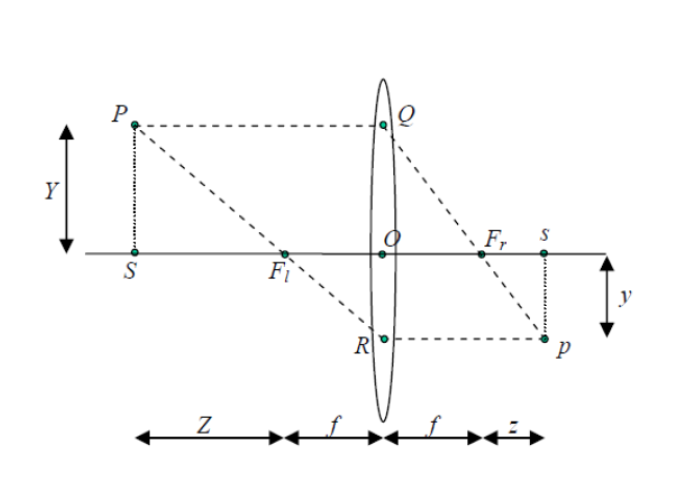
\includegraphics[width=0.76\textwidth]{source/tutorial-01-q1-optical-geometry.png}
  \caption{Q1 所用 thin-lens geometry（薄透镜几何）。来源：\textit{T1 Reference Solutions}，slide~2，裁切自原图。图中 $y$ 取倒立像高的正值。}
  \label{fig:sc4061-tut01-thin-lens}
\end{figure}

\begin{checkedsolution}
由穿过 left focal point（左焦点）并在折射后平行于光轴的光线，得到
\[
  \frac{Y}{Z}=\frac{y}{f}
  \quad\Longrightarrow\quad
  f=\frac{yZ}{Y}=\frac{y(\hat Z-f)}{Y}
  \quad\Longrightarrow\quad
  f=\frac{y\hat Z}{Y+y}.
\]
由入射时平行于光轴、折射后穿过 right focal point（右焦点）的光线，得到
\[
  \frac{Y}{f}=\frac{y}{z}
  \quad\Longrightarrow\quad
  f=\frac{Yz}{y}=\frac{Y(\hat z-f)}{y}
  \quad\Longrightarrow\quad
  f=\frac{Y\hat z}{Y+y}.
\]
两式相等，因此
\[
  \boxed{y\hat Z=Y\hat z}
  \qquad\Longleftrightarrow\qquad
  \boxed{\frac{Y}{\hat Z}=\frac{y}{\hat z}}.
\]
直角三角形 $PSO$ 与 $psO$ 的两条直角边成比例，故两三角形相似，对应的 $O$ 角相等；于是 $PO$ 与 $Op$ 是同一直线，证明 $P,O,p$ 共线。
\end{checkedsolution}

\textbf{检查点：}不能把“通过光心的光线不偏折”作为本题起点，否则会循环论证；必须先用另外两条主光线推出比例关系。

\exercisequestion{SC4061-TUT01-Q02}{Infinity Focus、Blur Diameter 与 Pinhole Trade-off}

\textbf{对应讲义：}
\relatedtopic{SC4061-L01-T04}{Depth of Field 与 Aperture Trade-off}

\subsubsection*{题目与思路}

相机 focused at infinity（聚焦于无穷远），所以 sensor plane（传感器平面）位于距透镜 $f$ 处。对距离透镜 $\hat Z$ 的有限物点 $P$，画出穿过 aperture edges（光圈边缘）的两条 outermost rays（最外侧光线），推导 sensor 上 blur circle diameter（弥散圆直径）$b$，并解释 aperture size（光圈大小）对 depth of field（景深）的影响以及 pinhole camera（针孔相机）的利弊。

\begin{figure}[htbp]
  \centering
  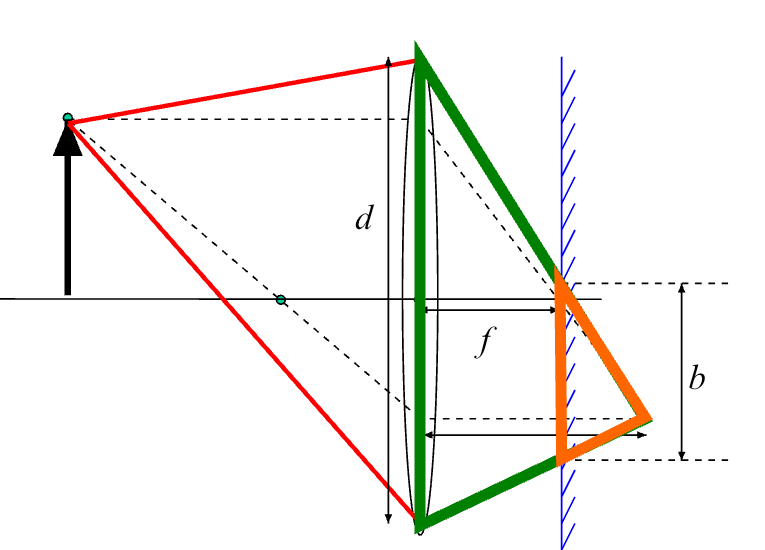
\includegraphics[width=0.88\textwidth]{source/tutorial-01-q2-infinity-focus.png}
  \caption{Q2 的outermost-ray diagram（最外侧光线图）。来源：\textit{T1 Reference Solutions}，slide~5，裁切自原图。有限物点应在 $\hat z>f$ 处聚焦，但sensor固定在 $f$ 处，因此在聚焦之前截得直径为 $b$ 的光束截面。}
  \label{fig:sc4061-tut01-infinity-focus}
\end{figure}

\begin{checkedsolution}
设该有限物点的正确 image distance（像距）为 $\hat z$。由 converging cone（会聚光锥）中的 similar triangles（相似三角形），
\[
  \frac{b}{d}=\frac{\hat z-f}{\hat z},
  \qquad
  b=d\left(1-\frac{f}{\hat z}\right).
\]
再由 thin-lens equation（薄透镜公式）
\[
  \frac{1}{\hat Z}+\frac{1}{\hat z}=\frac{1}{f}
  \quad\Longrightarrow\quad
  1-\frac{f}{\hat z}=\frac{f}{\hat Z},
\]
得到
\[
  \boxed{b=\frac{df}{\hat Z}}.
\]
在 $f$ 和 $\hat Z$ 固定时，$b\propto d$：larger aperture（更大光圈）产生更大的blur circle，因而depth of field更小；smaller aperture（更小光圈）产生更大的depth of field。

理想 pinhole camera 的优点是无需透镜且depth of field很大；缺点是 incoming light（进光量）很少，需要 longer exposure（更长曝光）或 higher ISO/gain（更高感光度/增益），分别容易造成 motion blur（运动模糊）或 noise（噪声）。针孔过小时还会受到 diffraction（衍射）限制，因此不能简单令孔径无限趋近于零。
\end{checkedsolution}

\textbf{检查点：}$b$ 与aperture diameter $d$ 成正比，而不是成反比；缩小光圈增加景深，但同时牺牲进光量。

\exercisequestion{SC4061-TUT01-Q03}{Fixed Sensor 下的 Thin-lens Defocus}

\textbf{对应讲义：}
\relatedtopic{SC4061-L01-T03}{Thin Lens Model 与 Magnification}；
\relatedtopic{SC4061-L01-T04}{Depth of Field 与 Aperture Trade-off}

\subsubsection*{题目与思路}

一台 thin-lens camera（薄透镜相机）的 focal length 为 $f=80\,\mathrm{mm}$，aperture diameter 为 $d=100\,\mathrm{mm}$。先对距离 $Z_1=1.5\,\mathrm{m}$ 的物体准确聚焦；随后不改变lens--sensor distance（透镜到传感器距离），拍摄距离 $Z_2=4\,\mathrm{m}$ 的第二个物体。求第一次聚焦时的sensor位置，以及第二个物点在sensor上的blur diameter。

\begin{checkedsolution}
统一使用毫米。第一次聚焦所需的像距为
\[
  z_1=\frac{fZ_1}{Z_1-f}
  =\frac{80\times1500}{1500-80}
  \approx\boxed{84.51\,\mathrm{mm}}.
\]
第二个物点真正的理想像距为
\[
  z_2=\frac{fZ_2}{Z_2-f}
  =\frac{80\times4000}{4000-80}
  \approx81.63\,\mathrm{mm}.
\]
由于camera is left untouched（相机保持不变），sensor仍位于 $z_1$，而第二个物点的光线已在 $z_2<z_1$ 处聚焦，随后再次发散到sensor。

\begin{figure}[htbp]
  \centering
  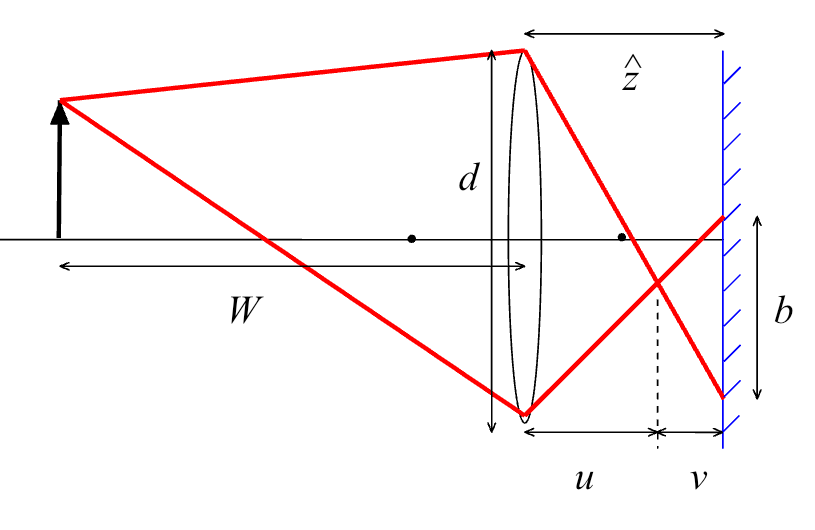
\includegraphics[width=0.88\textwidth]{source/tutorial-01-q3-fixed-sensor.png}
  \caption{Q3(b) 的fixed-sensor geometry（固定传感器几何）。来源：\textit{T1 Reference Solutions}，slide~9，裁切自原图。实际像点位于sensor之前，光线穿过它后再次发散，在sensor上形成blur circle。}
  \label{fig:sc4061-tut01-fixed-sensor-defocus}
\end{figure}

由 actual focus（实际焦点）两侧的similar triangles，
\[
  \frac{b}{d}=\frac{z_1-z_2}{z_2}
  \quad\Longrightarrow\quad
  b=d\frac{z_1-z_2}{z_2}
  \approx\boxed{3.52\,\mathrm{mm}}.
\]
Reference solution 中的 $3.53\,\mathrm{mm}$ 来自intermediate rounding（中间步骤取整）。
\end{checkedsolution}

\textbf{检查点：}“相机保持不变”固定的是sensor位置 $z_1$，不是第二个物点的理想像距；物体更远时 $z_2$ 更接近 $f$，所以本题中焦点位于sensor之前。

\exercisequestion{SC4061-TUT01-Q04}{Perceptron 迭代直至收敛}

\textbf{对应讲义：}
\relatedtopic{SC4061-L02-T03}{Perceptron Learning Rule}

\subsubsection*{题目与思路}

对 augmented samples（增广样本）
\[
  \tilde{\bm x}_1=(3,3,1)^{\mathsf T}\in c_1,
  \qquad
  \tilde{\bm x}_2=(1,1,1)^{\mathsf T}\in c_2,
\]
采用 $\alpha=1$、$\bm w(1)=\bm0$，按 $\tilde{\bm x}_1,\tilde{\bm x}_2$ 的顺序循环训练。$c_1$ 要求 $\bm w^{\mathsf T}\tilde{\bm x}>0$；$c_2$ 要求 $\bm w^{\mathsf T}\tilde{\bm x}<0$。等于零不算正确分类。

\begin{checkedsolution}
Misclassified $c_1$ sample（被错分的$c_1$样本）令 $\bm w\leftarrow\bm w+\tilde{\bm x}$；misclassified $c_2$ sample 令 $\bm w\leftarrow\bm w-\tilde{\bm x}$。全部迭代如下：

\begin{center}
\small
\begin{tabular}{@{}cclcl@{}}
  \toprule
  $k$ & 输入 & $\bm w(k)^{\mathsf T}\tilde{\bm x}$ & 操作 & $\bm w(k+1)^{\mathsf T}$ \\
  \midrule
  1  & $\tilde{\bm x}_1$ & $0$  & $+\tilde{\bm x}_1$ & $(3,3,1)$ \\
  2  & $\tilde{\bm x}_2$ & $7$  & $-\tilde{\bm x}_2$ & $(2,2,0)$ \\
  3  & $\tilde{\bm x}_1$ & $12$ & no update & $(2,2,0)$ \\
  4  & $\tilde{\bm x}_2$ & $4$  & $-\tilde{\bm x}_2$ & $(1,1,-1)$ \\
  5  & $\tilde{\bm x}_1$ & $5$  & no update & $(1,1,-1)$ \\
  6  & $\tilde{\bm x}_2$ & $1$  & $-\tilde{\bm x}_2$ & $(0,0,-2)$ \\
  7  & $\tilde{\bm x}_1$ & $-2$ & $+\tilde{\bm x}_1$ & $(3,3,-1)$ \\
  8  & $\tilde{\bm x}_2$ & $5$  & $-\tilde{\bm x}_2$ & $(2,2,-2)$ \\
  9  & $\tilde{\bm x}_1$ & $10$ & no update & $(2,2,-2)$ \\
  10 & $\tilde{\bm x}_2$ & $2$  & $-\tilde{\bm x}_2$ & $(1,1,-3)$ \\
  \bottomrule
\end{tabular}
\end{center}

最终
\[
  \bm w(11)=\boxed{(1,1,-3)^{\mathsf T}},
\]
且
\[
  \bm w(11)^{\mathsf T}\tilde{\bm x}_1=3>0,
  \qquad
  \bm w(11)^{\mathsf T}\tilde{\bm x}_2=-1<0,
\]
所以已经收敛，decision boundary（决策边界）为
\[
  \boxed{x_1+x_2-3=0}.
\]
若程序必须额外扫描一个完整epoch（轮次）才能检测收敛，则会再得到 $\bm w(12)=\bm w(13)=\bm w(11)$，但不会产生新的权重。
\end{checkedsolution}

\textbf{检查点：}最后一个增广分量对应bias；判断$c_1/c_2$时必须使用严格的正号/负号条件，并记录分类正确时未发生变化的迭代。

\subsubsection*{本次 Tutorial 收口}

Q1--Q3沿同一条camera geometry（相机几何）主线，依次训练光心射线、infinity focus下的离焦，以及固定sensor下的blur diameter；Q4独立训练perceptron online update（感知机在线更新）。复习时应优先掌握三个判断：先确认sensor固定在哪个image plane，blur diameter来自哪一组similar triangles，以及perceptron的类别符号约定。

% Tutorial set: 02
% Source: T2.pdf, Tutorial 2 (Image Enhancement in the Spatial Domain), Questions 1--3
% Reference: T2_Reference solutions.pptx, used for answer checking and qualitative plots
% Session date: 2026-09-01
% Human verified: Yes

\exercisegroup{SC4061-TUT02}{Tutorial 02：Spatial-domain Image Enhancement}
\label{tutorial:SC4061-TUT02}

\tutorialmeta
  {SC4061-TUT02}
  {2026-09-01}
  {T2.pdf，Questions 1--3；T2\_Reference solutions.pptx 仅用于核对}
  {三题均已作答、讨论并完成订正}
  {已确认（2026-09-01）}

\exercisequestion{SC4061-TUT02-Q01}{Monitor Gamma Calibration}

\textbf{对应讲义：}
\relatedtopic{SC4061-L03-T02}{Contrast、Gamma 与 Histogram Equalisation}

\subsubsection*{题目}

Monitor（显示器）的输入 gray level（灰度值）$r$ 与 photosensitive device（光敏设备）测得的输出 $s$ 被假设满足 power law（幂律）
\[
  s=cr^{\gamma}.
\]
实验给出 $100\mapsto0.24$ 与 $200\mapsto0.78$。（a）求 $\gamma$ 并判断曲线形状；（b）若输出单位改为 $24$ 与 $78$，判断估计的 $\gamma$ 是否改变；（c）说明该校准模型的不足。

\begin{checkedsolution}
两组方程相除可消去未知比例系数 $c$：
\[
  \frac{s_2}{s_1}=\left(\frac{r_2}{r_1}\right)^{\gamma},
  \qquad
  \gamma=\frac{\ln(s_2/s_1)}{\ln(r_2/r_1)}
  =\frac{\ln(13/4)}{\ln2}
  \approx\boxed{1.7004}.
\]
$\gamma>1$，故曲线 increasing and convex（单调递增且向上凸）。若所有输出统一乘以常数 $k$，ratio $ks_2/(ks_1)$ 不变，因此 $\gamma$ 不变，只会改变 $c$。

真实显示器通常不严格服从单一 power law；尤其在 $r=0$ 时仍可能存在 black offset（黑电平偏置）。较合理的简单模型可写为
\[
  s=b+cr^{\gamma},
\]
或使用 piecewise model / LUT（分段模型/查找表）。Ambient light、sensor calibration、screen position 与 colour channel 也会影响测量。
\end{checkedsolution}

\textbf{检查点：}改变统一的输入或输出单位不会改变由 ratios 求得的 $\gamma$；black offset 改变的是模型结构，不能仅靠重新估计 $c$ 修复。

\exercisequestion{SC4061-TUT02-Q02}{Step Edge 的 Box 与 Gaussian Smoothing}

\textbf{对应讲义：}
\relatedtopic{SC4061-L03-T04}{Box、Gaussian 与 Median Filtering}

\subsubsection*{题目}

一幅 grayscale image（灰度图像）左半为黑色、右半为白色，其横向 profile（剖面）是从 $0$ 跳至 $255$ 的 step edge（阶跃边缘），并假设 spatial continuous domain（连续空间域）。（a）画原图 histogram；（b）经 $L\times L$ box filter 后画输出 profile 与 histogram；（c）改用 Gaussian smoothing 后重复作图；（d）给出 MATLAB verification（验证）代码。

\begin{checkedsolution}
设edge位于 $x=0$：
\[
  r(x)=
  \begin{cases}
    0,&x<0,\\
    255,&x\ge0.
  \end{cases}
\]
原图只有两个 gray levels，normalized histogram 为
\[
  p_r(t)=\tfrac12\delta(t)+\tfrac12\delta(t-255).
\]

图像沿 $y$ 方向不变，因此 $L\times L$ box filter 可按一维宽度 $L$ 分析：
\[
  g_B(x)=
  \begin{cases}
    0,&x\le-L/2,\\[1mm]
    255\left(x/L+1/2\right),&-L/2<x<L/2,\\[1mm]
    255,&x\ge L/2.
  \end{cases}
\]
Step 被展开成宽度为 $L$ 的 linear ramp（线性斜坡）。大片纯黑/纯白区域仍产生 $0$ 与 $255$ 的 peaks；ramp slope 为常数 $255/L$，故中间 gray levels 对应相同空间宽度，在 histogram 中形成 uniform plateau（均匀平台）。

Gaussian kernel 与step的卷积为 Gaussian CDF：
\[
  g_G(x)=255\Phi\!\left(\frac{x}{\sigma}\right)
  =\frac{255}{2}\left[1+\operatorname{erf}\!\left(\frac{x}{\sqrt2\sigma}\right)\right].
\]
其profile为smooth S-curve（平滑S形曲线）。由变量变换
\[
  p_g(t)\propto\left|\frac{dx}{dt}\right|
  =\frac{1}{|dg_G/dx|},
\]
profile在中间斜率最大，因此中间gray levels较少；两端斜率小，因此histogram两端较高。Ideal Gaussian 具有无限support，只会渐近接近 $0$ 与 $255$；实际截断kernel会保留远离edge的纯黑/纯白区域，并在两端形成明显peaks。

\begin{figure}[htbp]
  \centering
  \resizebox{0.98\textwidth}{!}{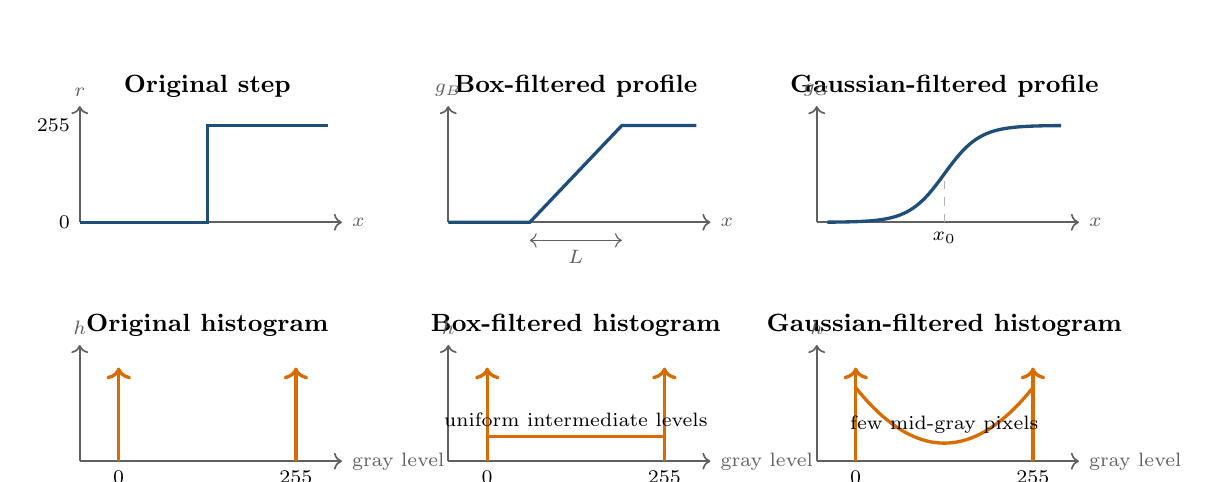
\begin{tikzpicture}[x=0.9cm,y=0.82cm,font=\scriptsize]
  \tikzset{
    axis/.style={->,semithick,gray!75!black},
    signal/.style={very thick,noteBlue},
    hist/.style={very thick,orange!85!black}
  }

  % Profiles
  \begin{scope}[shift={(0,3.7)}]
    \node[font=\small\bfseries] at (1.8,2.1) {Original step};
    \draw[axis] (0,0) -- (3.7,0) node[right] {$x$};
    \draw[axis] (0,0) -- (0,1.8) node[above] {$r$};
    \draw[signal] (0,0) -- (1.8,0) -- (1.8,1.5) -- (3.5,1.5);
    \node[left] at (0,0) {$0$};
    \node[left] at (0,1.5) {$255$};
  \end{scope}

  \begin{scope}[shift={(5.2,3.7)}]
    \node[font=\small\bfseries] at (1.8,2.1) {Box-filtered profile};
    \draw[axis] (0,0) -- (3.7,0) node[right] {$x$};
    \draw[axis] (0,0) -- (0,1.8) node[above] {$g_B$};
    \draw[signal] (0,0) -- (1.15,0) -- (2.45,1.5) -- (3.5,1.5);
    \draw[<->,gray!75!black] (1.15,-0.28) -- node[below] {$L$} (2.45,-0.28);
  \end{scope}

  \begin{scope}[shift={(10.4,3.7)}]
    \node[font=\small\bfseries] at (1.8,2.1) {Gaussian-filtered profile};
    \draw[axis] (0,0) -- (3.7,0) node[right] {$x$};
    \draw[axis] (0,0) -- (0,1.8) node[above] {$g_G$};
    \draw[signal,smooth,samples=80,domain=0.15:3.45]
      plot (\x,{1.5/(1+exp(-4*(\x-1.8)))});
    \draw[dashed,gray!60] (1.8,0) -- (1.8,0.75);
    \node[below] at (1.8,0) {$x_0$};
  \end{scope}

  % Histograms
  \begin{scope}[shift={(0,0)}]
    \node[font=\small\bfseries] at (1.8,2.1) {Original histogram};
    \draw[axis] (0,0) -- (3.7,0) node[right] {gray level};
    \draw[axis] (0,0) -- (0,1.8) node[above] {$h$};
    \draw[hist,->] (0.55,0) -- (0.55,1.45);
    \draw[hist,->] (3.05,0) -- (3.05,1.45);
    \node[below] at (0.55,0) {$0$};
    \node[below] at (3.05,0) {$255$};
  \end{scope}

  \begin{scope}[shift={(5.2,0)}]
    \node[font=\small\bfseries] at (1.8,2.1) {Box-filtered histogram};
    \draw[axis] (0,0) -- (3.7,0) node[right] {gray level};
    \draw[axis] (0,0) -- (0,1.8) node[above] {$h$};
    \draw[hist,->] (0.55,0) -- (0.55,1.45);
    \draw[hist,->] (3.05,0) -- (3.05,1.45);
    \draw[hist] (0.55,0.38) -- (3.05,0.38);
    \node[below] at (0.55,0) {$0$};
    \node[below] at (3.05,0) {$255$};
    \node[above] at (1.8,0.38) {uniform intermediate levels};
  \end{scope}

  \begin{scope}[shift={(10.4,0)}]
    \node[font=\small\bfseries] at (1.8,2.1) {Gaussian-filtered histogram};
    \draw[axis] (0,0) -- (3.7,0) node[right] {gray level};
    \draw[axis] (0,0) -- (0,1.8) node[above] {$h$};
    \draw[hist,->] (0.55,0) -- (0.55,1.45);
    \draw[hist,->] (3.05,0) -- (3.05,1.45);
    \draw[hist,smooth,samples=60,domain=0.55:3.05]
      plot (\x,{0.28+0.55*(\x-1.8)^2});
    \node[below] at (0.55,0) {$0$};
    \node[below] at (3.05,0) {$255$};
    \node[above] at (1.8,0.28) {few mid-gray pixels};
  \end{scope}
\end{tikzpicture}
}
  \caption{Q2 的profile与histogram对照。依据\textit{T2} Question 2及\textit{T2 Reference Solutions} slides 7--8重绘；histogram纵轴只表示定性频数。}
  \label{fig:sc4061-tut02-filter-profiles}
\end{figure}

\textbf{MATLAB verification：}
\begin{verbatim}
N = 512; L = 31; sigma = 5;
I = zeros(N); I(:, N/2+1:end) = 255;
B = imfilter(I, ones(L,L)/(L^2), 'replicate', 'same');
G = imgaussfilt(I, sigma, 'FilterSize', L, ...
                'Padding', 'replicate');

x = 1:N; row = N/2;
subplot(2,2,1); plot(x, I(row,:), x, B(row,:));
subplot(2,2,2); histogram(B(:), 0:256);
subplot(2,2,3); plot(x, I(row,:), x, G(row,:));
subplot(2,2,4); histogram(G(:), 0:256);
\end{verbatim}
\end{checkedsolution}

\textbf{检查点：}Profile 的纵轴是输出intensity，histogram的纵轴是pixel frequency；$g_B(0)=127.5$ 不等于“histogram在$0$处变为$127.5$”。

\exercisequestion{SC4061-TUT02-Q03}{Median Filter 对 Spikes 与 Step Edge 的作用}

\textbf{对应讲义：}
\relatedtopic{SC4061-L03-T04}{Box、Gaussian 与 Median Filtering}

\subsubsection*{题目}

给定1D signal
\[
  [2,6,53,10,7,4,107,103,104,109,57,102].
\]
其中包含两个spikes（尖峰）和一个step edge。（a）画出signal；（b）采用endpoint replication（端点复制）边界，对其施加3-element median filter并写出输出；（c）对输出再次施加同一filter；（d）说明若改用Gaussian filtering，spikes与edge如何变化；（e）说明何时median filtering更合适。

\begin{checkedsolution}
三元素中值滤波为
\[
  y_i=\operatorname{median}(x_{i-1},x_i,x_{i+1}),
  \qquad x_0=x_1,\quad x_{13}=x_{12}.
\]
第一次输出为
\[
  \boxed{[2,6,10,10,7,7,103,104,104,104,102,102]}.
\]
对该结果再次滤波，输出不再改变。两个isolated spikes被移除，而low-to-high step仍被保留。

Gaussian filtering使用weighted average（加权平均）：spike amplitude会减小，但异常值也会扩散到邻近位置；step edge会变宽、斜率降低。Median filtering更适合salt-and-pepper noise（椒盐噪声）或少量extreme outliers，并通常更能保留sharp edges。

Median能恢复正常值的条件是窗口内被污染样本少于一半；若3个元素中至少2个异常，median也会失败。此外，“第二次不再变化”只对本题signal成立，并非median filter普遍只需执行一次。
\end{checkedsolution}

\textbf{检查点：}Median filter是nonlinear filter（非线性滤波器），不能用convolution theorem分析；其robustness来自order statistic（次序统计量），而不是对异常值赋予较小线性权重。

\subsubsection*{本次 Tutorial 收口}

Q1训练power-law calibration与模型失配；Q2用profile slope解释smoothing后的histogram；Q3比较median与Gaussian对outlier和edge的不同影响。复习时优先掌握：ratio消去尺度、histogram density与profile slope成反比，以及median成功需要窗口内正常样本占多数。

% Tutorial set: 03
% Source: T3.pdf, Tutorial 3 (Image Enhancement in the Frequency Domain), Questions 1--3
% Reference: T3_Reference solutions.pptx, used only for answer checking
% Session date: 2026-09-08
% Human verified: Yes

\exercisegroup{SC4061-TUT03}{Tutorial 03：Frequency-domain Image Enhancement}
\label{tutorial:SC4061-TUT03}

\tutorialmeta
  {SC4061-TUT03}
  {2026-09-08}
  {T3.pdf，Questions 1--3；T3\_Reference solutions.pptx 仅用于核对}
  {三题均已完成推导、讨论并订正}
  {已确认（2026-09-08）}

\exercisequestion{SC4061-TUT03-Q01}{Spatial Mask、Frequency Response 与 Separability}

\textbf{对应讲义：}
\relatedtopic{SC4061-L04-T03}{FFT 与 Convolution Theorem}；
\relatedtopic{SC4061-L04-T05}{Low-pass、High-pass 与 Notch Filtering}

\subsubsection*{题目}

给定 spatial convolution mask（空间卷积核）
\[
  h(x,y)=\frac15
  \begin{bmatrix}
    0&1&0\\
    1&1&1\\
    0&1&0
  \end{bmatrix}.
\]
（a）利用 translation property（平移性质）推导其 frequency response（频率响应），并解释其 low-pass property（低通性质）。（b）若 $f(x,y)=f_1(x)f_2(y)$，证明二维 Fourier transform 可分离，并说明该性质对 convolution 的意义。

\begin{checkedsolution}
将 mask 写成 shifted impulses（移位冲激）之和：
\[
  h(x,y)=\frac15\bigl[
  \delta(x,y)+\delta(x-1,y)+\delta(x+1,y)
  +\delta(x,y-1)+\delta(x,y+1)\bigr].
\]
由
\[
  f(x-x_0,y-y_0)
  \Longleftrightarrow
  F(u,v)e^{-j2\pi(ux_0/M+vy_0/N)},
\]
得到
\begin{align*}
  H(u,v)
  &=\frac15\left(1+e^{-j2\pi u/M}+e^{j2\pi u/M}
  +e^{-j2\pi v/N}+e^{j2\pi v/N}\right)\\
  &=\boxed{\frac15\left(1+2\cos\frac{2\pi u}{M}
  +2\cos\frac{2\pi v}{N}\right)}.
\end{align*}
特别地，$H(0,0)=1$，所以 DC component（直流分量）完整保留。该 mask 对中心及四邻域求平均；slow variation（缓慢变化）的各项近似同相，而 rapid oscillation（快速振荡）会在求和中相消，因此总体属于 low-pass filter。它并非 ideal、radially monotone low-pass：例如 $H(M/2,N/2)=-3/5$，仍存在 side lobes（旁瓣）与 phase reversal（相位反转）。

对 separable signal（可分离信号），
\begin{align*}
F(u,v)
&=\sum_{y=0}^{N-1}\sum_{x=0}^{M-1}
f_1(x)f_2(y)e^{-j2\pi ux/M}e^{-j2\pi vy/N}\\
&=\left(\sum_{x=0}^{M-1}f_1(x)e^{-j2\pi ux/M}\right)
\left(\sum_{y=0}^{N-1}f_2(y)e^{-j2\pi vy/N}\right)\\
&=\boxed{F_1(u)F_2(v)}.
\end{align*}
若 filter 也满足 $h(x,y)=h_1(x)h_2(y)$，二维 convolution 可依次执行两个 one-dimensional convolutions（一维卷积）。对 $K\times K$ kernel，每个 pixel 的主要乘法量由约 $K^2$ 降为 $2K$。
\end{checkedsolution}

\textbf{检查点：}``averaging mask'' 足以说明总体 smoothing tendency（平滑倾向），但不意味着 $|H(u,v)|$ 沿任意径向都严格单调。

\exercisequestion{SC4061-TUT03-Q02}{Gaussian Fourier Transform 与 Domain Scaling}

\textbf{对应讲义：}
\relatedtopic{SC4061-L04-T02}{DFT、IDFT 与 Spectrum}；
\relatedtopic{SC4061-L04-T05}{Low-pass、High-pass 与 Notch Filtering}

\subsubsection*{题目}

在
\[
  e^{-\pi x^2}\Longleftrightarrow e^{-\pi u^2},
  \qquad
  f(ax)\Longleftrightarrow \frac1{|a|}F\!\left(\frac ua\right)
\]
的 convention 下，证明 standard deviation（标准差）为 $\sigma$ 的 unit-amplitude Gaussian（单位峰值高斯函数）仍变换为 Gaussian，并求其 frequency-domain amplitude 与 standard deviation。

\begin{checkedsolution}
令 $\sigma>0$，将空间域函数配成已知形式：
\[
  e^{-x^2/(2\sigma^2)}=e^{-\pi(ax)^2},
  \qquad
  \pi a^2=\frac1{2\sigma^2},
  \qquad
  a=\frac1{\sqrt{2\pi}\,\sigma}.
\]
使用 scaling theorem：
\begin{align*}
  e^{-x^2/(2\sigma^2)}
  &\Longleftrightarrow
  \frac1a e^{-\pi(u/a)^2}\\
  &=\sqrt{2\pi}\,\sigma\,
  e^{-2\pi^2\sigma^2u^2}\\
  &=\boxed{\sqrt{2\pi}\,\sigma
  \exp\!\left(-\frac{u^2}{2\alpha^2}\right)},
  \qquad
  \boxed{\alpha=\frac1{2\pi\sigma}}.
\end{align*}
前面的 coefficient（系数）给出 frequency-domain amplitude；指数中的 $\alpha$ 给出 width（宽度），两者作用不同。还可用
\[
  F(0)=\int_{-\infty}^{\infty}e^{-x^2/(2\sigma^2)}\,dx
  =\sqrt{2\pi}\,\sigma
\]
检查 amplitude。空间域越宽，频域越窄，并满足
\[
  \boxed{\sigma\alpha=\frac1{2\pi}}.
\]
该常数依赖这里采用的 $e^{-j2\pi ux}$ Fourier convention；更换 convention 会移动 $2\pi$。
\end{checkedsolution}

\textbf{检查点：}本题空间域 Gaussian 没有除以 $\sqrt{2\pi}\sigma$，所以它的面积和 $F(0)$ 都随 $\sigma$ 增大；不能只改指数而漏掉 scaling coefficient。

\exercisequestion{SC4061-TUT03-Q03}{Second Difference 的 Directional High-pass Response}

\textbf{对应讲义：}
\relatedtopic{SC4061-L04-T05}{Low-pass、High-pass 与 Notch Filtering}；
\relatedtopic{SC4061-L05-T04}{Image Edges、Gradient 与 Curvature}

\subsubsection*{题目}

设
\[
  g(x,y)=f(x+1,y)+f(x-1,y)-2f(x,y).
\]
推导 $G(u,v)$ 与 $F(u,v)$ 的关系，判断 filter type（滤波器类型），并说明其方向性。

\begin{checkedsolution}
两次 spatial shift 分别产生相反的 phase factor：
\begin{align*}
  G(u,v)
  &=\left(e^{j2\pi u/M}+e^{-j2\pi u/M}-2\right)F(u,v)\\
  &=\left(2\cos\frac{2\pi u}{M}-2\right)F(u,v)\\
  &=\boxed{-4\sin^2\!\left(\frac{\pi u}{M}\right)F(u,v)}.
\end{align*}
因此 transfer function（传递函数）为
\[
  H(u,v)=-4\sin^2\!\left(\frac{\pi u}{M}\right),
  \qquad
  |H(u,v)|=4\sin^2\!\left(\frac{\pi u}{M}\right).
\]
$H(0,v)=0$，而 $|H(M/2,v)|=4$；它消除沿 $x$ 不变的成分并增强沿 $x$ 的快速变化，所以是 directional high-pass filter（方向性高通滤波器）。负号改变 response sign/phase，不改变 pass type。

原始 DFT array 中 $u=0,1,\ldots,M-1$ 的后半段代表 negative frequencies（负频率）：
\[
  \widetilde u=
  \begin{cases}
    u,&0\le u\le M/2,\\
    u-M,&M/2<u<M.
  \end{cases}
\]
例如 $u=M-1$ 实际是低频 $-1$，而不是更高的正频率。因此响应从 $u=M/2$ 向 $u=M$ 降低，是 frequency wrapping（频率回绕）后的对称部分；在 centred frequency axis 上，$|H|$ 随 $|\widetilde u|$ 增大，在 Nyquist frequency 处最大。

\begin{figure}[htbp]
  \centering
  \resizebox{0.96\textwidth}{!}{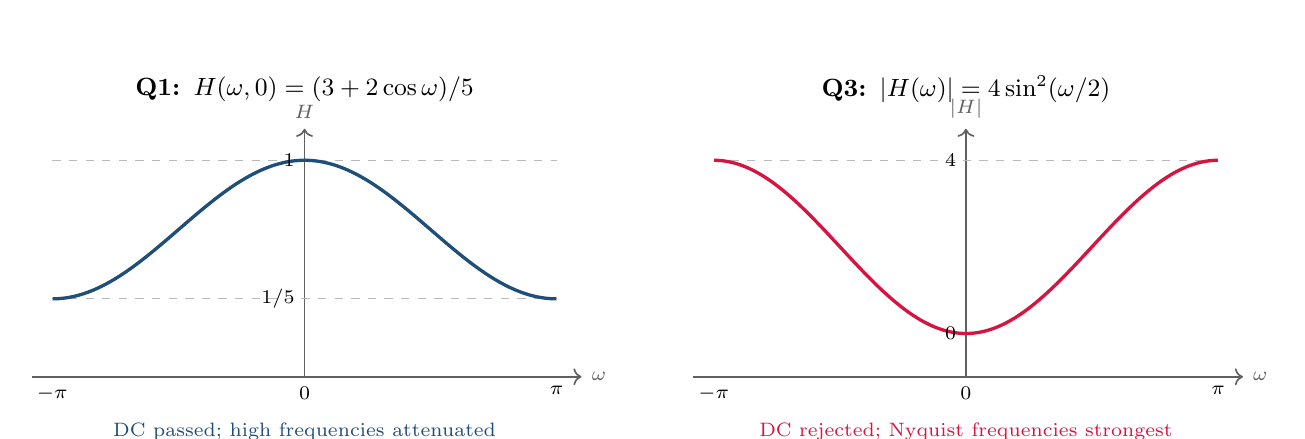
\begin{tikzpicture}[x=1.05cm,y=1.0cm,font=\scriptsize]
  \tikzset{
    axis/.style={->,semithick,gray!75!black},
    lowpass/.style={very thick,noteBlue},
    highpass/.style={very thick,ntuRed},
    guide/.style={dashed,gray!55}
  }

  \begin{scope}[shift={(0,0)}]
    \node[font=\small\bfseries] at (3.3,3.65) {Q1: $H(\omega,0)=(3+2\cos\omega)/5$};
    \draw[axis] (0,0) -- (6.65,0) node[right] {$\omega$};
    \draw[axis] (3.3,0) -- (3.3,3.15) node[above] {$H$};
    \draw[guide] (0.25,2.75) -- (6.35,2.75);
    \draw[guide] (0.25,0.99) -- (6.35,0.99);
    \draw[lowpass,smooth,samples=100,domain=-3.14159:3.14159]
      plot ({3.3+0.97*\x},{0.55+2.2*(3+2*cos(\x r))/5});
    \node[left] at (3.3,2.75) {$1$};
    \node[left] at (3.3,0.99) {$1/5$};
    \node[below] at (0.25,0) {$-\pi$};
    \node[below] at (3.3,0) {$0$};
    \node[below] at (6.35,0) {$\pi$};
    \node[align=center,noteBlue] at (3.3,-0.7) {DC passed; high frequencies attenuated};
  \end{scope}

  \begin{scope}[shift={(8.0,0)}]
    \node[font=\small\bfseries] at (3.3,3.65) {Q3: $|H(\omega)|=4\sin^2(\omega/2)$};
    \draw[axis] (0,0) -- (6.65,0) node[right] {$\omega$};
    \draw[axis] (3.3,0) -- (3.3,3.15) node[above] {$|H|$};
    \draw[guide] (0.25,2.75) -- (6.35,2.75);
    \draw[highpass,smooth,samples=100,domain=-3.14159:3.14159]
      plot ({3.3+0.97*\x},{0.55+0.55*4*(sin(\x/2 r))^2});
    \node[left] at (3.3,2.75) {$4$};
    \node[left] at (3.3,0.55) {$0$};
    \node[below] at (0.25,0) {$-\pi$};
    \node[below] at (3.3,0) {$0$};
    \node[below] at (6.35,0) {$\pi$};
    \node[align=center,ntuRed] at (3.3,-0.7) {DC rejected; Nyquist frequencies strongest};
  \end{scope}
\end{tikzpicture}
}
  \caption{Q1 与 Q3 的一维 frequency-response cross-sections（频率响应截面）。横轴使用 centred angular frequency，避免把 raw DFT index 的回绕误认为更高频率。}
  \label{fig:sc4061-tut03-frequency-responses}
\end{figure}

$g$ 是沿 $x$ 的 exact central second difference（精确中心二阶差分）；当 sampling interval 为 $1$ 且 $f$ 足够平滑时，才近似 $\partial^2f/\partial x^2$，不能直接写成严格相等。

方向名称依赖 coordinate convention（坐标约定）：该算子始终检测 intensity 沿 $x$ 变化的边界，edge tangent 与 $x$ 方向垂直。按本课程常用的 image-matrix convention（$x$ 为 row、从上到下），它响应 horizontal edges（水平边缘）；若采用 Cartesian convention（$x$ 从左到右），同一算子则响应 vertical edges（竖直边缘）。
\end{checkedsolution}

\textbf{检查点：}判断 DFT filter type 时看 centred signed frequency（中心化带符号频率）上的 $|H|$，不能把 raw index $u$ 的数值大小直接当作频率高低。

\subsubsection*{本次 Tutorial 收口}

Q1 将 local averaging mask 转为 frequency response，并利用 separability 把二维运算拆成两个一维运算；Q2 展示 Gaussian 在 Fourier transform 下保持 Gaussian 形状，但 amplitude 与 width 按 scaling theorem 同时变化；Q3 把 central second difference 写成 directional high-pass response。复习时优先掌握：shift 对应 phase factor、$G=HF$、空间域与频域 Gaussian 宽度成反比，以及 raw DFT indices 的后半段代表 negative frequencies。

% Tutorial set: 04
% Source: T4.pdf, Tutorial 4 (Image Edge Processing), Questions 1--3
% Reference: T4_Reference solutions.pptx, used only for answer checking
% Session date: 2026-09-15
% Human verified: Yes

\exercisegroup{SC4061-TUT04}{Tutorial 04：Image Edge Processing}
\label{tutorial:SC4061-TUT04}

\tutorialmeta
  {SC4061-TUT04}
  {2026-09-15}
  {T4.pdf，Questions 1--3；T4\_Reference solutions.pptx 仅用于核对}
  {三题均已作答、讨论并完成订正}
  {已确认（2026-09-15）}

\exercisequestion{SC4061-TUT04-Q01}{Sobel Mask 的 Separable Implementation}

\textbf{对应讲义：}
\relatedtopic{SC4061-L05-T05}{Prewitt 与 Sobel Gradient Filters}

\subsubsection*{题目}

证明 Sobel masks（Sobel 卷积核）可以由一次一维 differencing（差分）和一次正交方向的一维 smoothing（平滑）依次实现：差分核为 $[-1,0,1]^{\mathsf T}$ 或其水平版本，平滑核为 $[1,2,1]$ 或其垂直版本。

\begin{checkedsolution}
令水平差分与垂直平滑分别为
\[
  d_x=\begin{bmatrix}-1&0&1\end{bmatrix},\qquad
  s_y=\begin{bmatrix}1&2&1\end{bmatrix}^{\mathsf T}.
\]
二者的 outer product（外积）为
\[
  K_x=s_y d_x
  =\begin{bmatrix}
    -1&0&1\\
    -2&0&2\\
    -1&0&1
  \end{bmatrix}.
\]
$K_x$ 计算沿 $x$ 的 intensity difference（强度差），因此响应 vertical edges（竖直边缘）。交换两个方向可得
\[
  K_y=d_y s_x
  =\begin{bmatrix}
    -1&-2&-1\\
    0&0&0\\
    1&2&1
  \end{bmatrix},
\]
它计算沿 $y$ 的差分并响应 horizontal edges（水平边缘）。

由 convolution（卷积）的结合律，二维 Sobel filtering 可写成
\[
  f*K_x=(f*d_x)*s_y=(f*s_y)*d_x.
\]
因此先差分再平滑或先平滑再差分都得到同一二维结果。若软件实际执行 cross-correlation（互相关）而没有翻转 kernel，输出可能整体变号；这会改变 gradient orientation（梯度朝向）$180^\circ$，但不会改变 gradient magnitude 或 edge location。
\end{checkedsolution}

\exercisequestion{SC4061-TUT04-Q02}{LoG Kernel、Filtering Response 与 Zero Crossing}

\textbf{对应讲义：}
\relatedtopic{SC4061-L05-T06}{Laplacian of Gaussian 与 Zero Crossing}

\subsubsection*{题目}

令
\[
  h(r)=-\exp\!\left(-\frac{r^2}{2\sigma^2}\right),
  \qquad r^2=x^2+y^2.
\]
（a）详细推导 $\nabla^2h(r)$。（b）使用离散 LoG kernel
\[
  L=\begin{bmatrix}
    0&0&-1&0&0\\
    0&-1&-2&-1&0\\
    -1&-2&16&-2&-1\\
    0&-1&-2&-1&0\\
    0&0&-1&0&0
  \end{bmatrix}
\]
对两幅 $12\times13$ 图像做 valid filtering（不补零，只保留 kernel 完全落入图像的位置），并比较结果。两幅图像的 12 行分别重复以下 row profiles：
\[
  x_{\mathrm{step}}=
  [0,0,0,0,0,0,1,1,1,1,1,1,1],
\]
\[
  x_{\mathrm{ramp}}=
  [0,0,0,0,0,0,0.5,1,1,1,1,1,1].
\]

\begin{checkedsolution}
记 $q=(x^2+y^2)/(2\sigma^2)$。链式法则给出
\[
  \frac{\partial h}{\partial x}
  =\frac{x}{\sigma^2}e^{-q},\qquad
  \frac{\partial^2h}{\partial x^2}
  =-\frac{x^2-\sigma^2}{\sigma^4}e^{-q}.
\]
同理，
\[
  \frac{\partial^2h}{\partial y^2}
  =-\frac{y^2-\sigma^2}{\sigma^4}e^{-q}.
\]
所以
\[
  \boxed{
  \nabla^2h(r)
  =-\frac{r^2-2\sigma^2}{\sigma^4}
  \exp\!\left(-\frac{r^2}{2\sigma^2}\right)}.
\]
题目采用的是 negative unnormalised Gaussian（负的未归一化高斯函数），所以 kernel 中心为正。若从通常的 positive normalised Gaussian
\[
  G_\sigma(r)=\frac{1}{2\pi\sigma^2}
  e^{-r^2/(2\sigma^2)}
\]
出发，则
\[
  \nabla^2G_\sigma(r)
  =\frac{r^2-2\sigma^2}{2\pi\sigma^6}
  e^{-r^2/(2\sigma^2)},
\]
与题目 convention（约定）整体异号并多一个归一化系数；二者的 zero crossing 都位于 $r=\sqrt2\sigma$。

因为图像的每一行都相同，二维 filtering 可约化为一维。将 $L$ 的每列求和，得到 effective kernel（等效卷积核）
\[
  \ell=[-1,-4,10,-4,-1].
\]
输入高度与宽度分别从 $12,13$ 变成
\[
  12-5+1=8,\qquad 13-5+1=9.
\]
每个输出均有 8 个相同行，其 row profiles 为
\[
  \boxed{y_{\mathrm{step}}
  =[0,0,-1,-5,5,1,0,0,0]},
\]
\[
  \boxed{y_{\mathrm{ramp}}
  =[0,0,-0.5,-3,0,3,0.5,0,0]}.
\]
Reference solutions 的渐变响应末尾漏写了一个 $0$；由 $13-5+1=9$ 可确认完整输出必须有 9 列。

Abrupt step（突变阶跃）产生较强的正负 double-lobe response（双瓣响应），zero crossing 位于 $-5$ 与 $5$ 之间。加入 $0.5$ 的过渡后，响应峰值降至 $\pm3$，并在边缘中心出现一个精确的零。LoG 以 sign change（符号变化）定位边缘；整体改变 kernel sign 不改变 zero-crossing location。
\end{checkedsolution}

\exercisequestion{SC4061-TUT04-Q03}{Hough Line Geometry 与 Parameter-space Voting}

\textbf{对应讲义：}
\relatedtopic{SC4061-L06-T01}{Edgel Linking 与 Hough Line Geometry}；
\relatedtopic{SC4061-L06-T02}{Image--Hough Duality、Voting 与 Generalization}

\subsubsection*{题目}

直线可写为
\[
  \rho=x\cos\theta+y\sin\theta.
\]
（a）从几何上说明 $\rho$ 与 $\theta$；（b）在可行时将直线写成 $y=mx+c$；（c）固定图像点 $(x,y)$，证明它在 $(\theta,\rho)$ parameter space（参数空间）中对应 sinusoid（正弦曲线）$\rho=K\cos\alpha$；（d）解释两条以及多条 sinusoids 的交点分别对应什么图像结构。

\begin{checkedsolution}
直线的单位法向量为
\[
  \mathbf n=(\cos\theta,\sin\theta)^{\mathsf T}.
\]
$\theta$ 是 $\mathbf n$ 与 $x$ 轴的夹角，$\rho$ 是原点到直线的 signed distance（有符号距离），而距离原点最近的直线点为 $\rho\mathbf n$。

当 $\sin\theta\ne0$ 时，
\[
  y=-\frac{\cos\theta}{\sin\theta}x
  +\frac{\rho}{\sin\theta}
  =-\cot\theta\,x+\rho\csc\theta.
\]
因此 $m=-\cot\theta$，$c=\rho\csc\theta$。当 $\sin\theta=0$ 时，直线为 $x=\rho/\cos\theta$，即 vertical line（竖直线），不能写成具有有限 slope 的 $y=mx+c$。Normal form（法线式）正是通过 $\rho,\theta$ 避免 slope singularity（斜率奇点）。

对固定点 $(x,y)$，令
\[
  R=\sqrt{x^2+y^2},\qquad
  \phi=\operatorname{atan2}(y,x),\qquad
  x=R\cos\phi,\quad y=R\sin\phi.
\]
代入直线方程：
\begin{align*}
  \rho(\theta)
  &=R\cos\phi\cos\theta+R\sin\phi\sin\theta\\
  &=\boxed{R\cos(\theta-\phi)}.
\end{align*}
所以题目中的 $K=R$，而 $\alpha$ 可取 $\theta-\phi$；由于 cosine（余弦）是偶函数，写成 $R\cos(\phi-\theta)$ 也完全等价。Reference solutions 使用 $\tan^{-1}(y/x)$ 表示 $\phi$，但严格实现时应使用 $\operatorname{atan2}(y,x)$，否则不能正确区分象限，且 $x=0$ 时会发生除零。

每个 edgel（边缘像素）在 Hough space 中给所有经过它的直线投票，因此形成一条 sinusoid。两条 sinusoids 的交点表示两个图像点共同确定的一条直线；多条 sinusoids 在同一 $(\rho,\theta)$ 附近相交，表示多个 edgels 共线，并在 accumulator（累加器）中形成较强 peak。离散实现中受 parameter quantisation（参数量化）和噪声影响，投票通常形成邻近 bins 的峰簇，而不是理想的精确交点。

\begin{figure}[htbp]
  \centering
  \resizebox{0.94\textwidth}{!}{\begin{tikzpicture}[font=\small,>=Latex]
  \begin{scope}[xshift=0cm]
    \draw[->,thick] (-0.3,0) -- (3.4,0) node[right] {$x$};
    \draw[->,thick] (0,-1.3) -- (0,1.7) node[above] {$y$};
    \draw[very thick,noteBlue] (1,-1.15) -- (1,1.45);
    \foreach \yy/\cc in {-0.7/ntuRed,0/orange!85!black,0.7/teal!75!black} {
      \fill[\cc] (1,\yy) circle (3.2pt);
    }
    \node[align=center] at (1.65,-1.55) {image space\\共线 edgels};
  \end{scope}

  \draw[->,very thick,gray!65] (3.7,0.2) -- (5.1,0.2)
    node[midway,above,align=center] {vote};

  \begin{scope}[xshift=5.7cm,x=0.035cm,y=1.05cm]
    \draw[->,thick] (-85,0) -- (88,0) node[right] {$\theta$};
    \draw[->,thick] (0,-1.35) -- (0,1.7) node[above] {$\rho$};
    \draw[ntuRed,very thick,samples=90,domain=-80:80,smooth]
      plot (\x,{cos(\x)-0.7*sin(\x)});
    \draw[orange!85!black,very thick,samples=90,domain=-80:80,smooth]
      plot (\x,{cos(\x)});
    \draw[teal!75!black,very thick,samples=90,domain=-80:80,smooth]
      plot (\x,{cos(\x)+0.7*sin(\x)});
    \fill[noteBlue] (0,1) circle (3.5pt);
    \draw[dashed,noteBlue] (0,0) -- (0,1);
    \node[anchor=west,noteBlue] at (5,1.18) {peak $(\theta^*,\rho^*)$};
    \node[align=center] at (0,-1.65) {Hough space\\sinusoids intersect};
  \end{scope}
\end{tikzpicture}
}
  \caption{Q3 的 image--Hough duality：image space 中的共线 edgels 在 Hough space 中产生共同参数峰。图为依据课程内容绘制的原创示意图。}
  \label{fig:sc4061-tut04-hough-voting}
\end{figure}
\end{checkedsolution}

\subsubsection*{本次 Tutorial 收口}

Q1 利用 separability（可分离性）把二维 Sobel convolution 拆为差分与平滑；Q2 连接 continuous LoG derivation、discrete filtering response 与 zero crossing，并用输出尺寸发现参考答案漏项；Q3 在 image space 与 Hough space 之间切换变量角色，以 signed normal form 统一表示普通直线和竖直线。复习时应优先保留 kernel direction、sign convention、valid-output size、$\sin\theta=0$ 特例与 $\operatorname{atan2}$ 的象限信息。

% Based on templates/tutorial.tex; finished notes omit conversational checks.
% Source: LEC05 Image Segmentation - Tutorial Problems.pdf, PDF p. 1, Q1--Q3.
% Q1 supporting lecture: LEC05 Image Segmentation - 2026.pdf, p. 34.
% No official answer key supplied. Q3 uses approximate diagram coordinates;
% its assignment/update sequence was independently checked numerically.
% Session: 2026-10-20, teaching Week 10. User reviewed and approved publication.

\begingroup
\renewcommand{\recordid}[1]{}
\renewcommand{\relatedtopic}[2]{\hyperref[topic:#1]{#2}}

\exercisegroup{SC4061-TUT05}{Tutorial 05：Image Segmentation}
\label{tutorial:SC4061-TUT05}

{\small 2026-10-20（第十教学周）。来源：\emph{LEC05 Image Segmentation -- Tutorial Problems}，PDF p.~1，Questions 1--3；滤波特征的局部聚合参照 \emph{LEC05 Image Segmentation -- 2026} p.~34。原文件无参考答案；推导与迭代已核对，笔记已确认。}

\exercisequestion{SC4061-TUT05-Q01}{用 Filter Bank 分割纹理图像}

\textbf{对应讲义：}\relatedtopic{SC4061-L08-T01}{Gabor 滤波器与纹理特征向量}；
\relatedtopic{SC4061-L08-T02}{K-means 纹理聚类}。

\textbf{题目。}说明如何利用 filter bank（滤波器组）分割具有不同纹理的图像。

\begin{checkedsolution}
纹理差异体现在局部结构的方向、尺度和空间频率。选择对这些性质具有不同响应的滤波器，例如一组不同方向和波长的 Gabor filters，分别作用于同一幅原图：
\[
  g_j(x,y)=(f*h_j)(x,y),\qquad j=1,\ldots,M.
\]
每个滤波器产生一张响应图。按讲义 p.~34，在各响应图的局部窗口 $\mathcal N$ 内聚合幅值，再拼接成同一个像素的特征向量：
\[
  \tau_j(x,y)=\sum_{(u,v)\in\mathcal N}|g_j(x+u,y+v)|,\qquad
  \bm\tau(x,y)=\bigl[\tau_1(x,y),\ldots,\tau_M(x,y)\bigr]^{\mathsf T}.
\]
幅值聚合避免振荡响应正负抵消，并描述邻域纹理。将每个像素的 $\bm\tau(x,y)$ 视为特征空间中的一个点，用 K-means 等算法将相似特征聚为一类，最后把簇标签放回对应的像素位置，得到分割图。

\[
  \boxed{\text{原图}}
  \ \longrightarrow\ \boxed{M\text{ 张滤波响应图}}
  \ \longrightarrow\ \boxed{\text{逐像素 }M\text{ 维特征}}
  \ \longrightarrow\ \boxed{K\text{ 类标签图}}.
\]
滤波器数 $M$ 决定特征维数，簇数 $K$ 决定输出类别数。聚类比较的是纹理特征；同一簇的像素未必在图像中连成一个区域。
\end{checkedsolution}

\exercisequestion{SC4061-TUT05-Q02}{Otsu：灰度统计量与加权均值}

\textbf{对应讲义：}\relatedtopic{SC4061-L07-T02}{区域统计与归一化直方图}；
\relatedtopic{SC4061-L07-T03}{Global Thresholding 与 Otsu 方法}。
\par\nopagebreak[4]

\textbf{题目。}设 $p(r)$ 描述图像中灰度 $r\in\{0,\ldots,255\}$ 的概率。
(a) 写出与阈值无关的整体均值 $\mu$ 和方差 $\sigma^2$；
(b) 解释 Otsu 目标 $\sigma_w^2=q_L\sigma_L^2+q_H\sigma_H^2$ 的各项；
(c) 给定阈值 $T$，证明 $\mu=q_L\mu_L+q_H\mu_H$。

\begin{checkedsolution}
\textbf{(a) 整体均值与方差。}令图像有 $n$ 个像素，其中 $h(r)$ 个像素的灰度为 $r$。归一化直方图为 $p(r)=h(r)/n$，满足 $\sum_{r=0}^{255}p(r)=1$。因此
\[
  \boxed{\mu=\sum_{r=0}^{255}r\,p(r)},\qquad
  \boxed{\sigma^2=\sum_{r=0}^{255}(r-\mu)^2p(r)}.
\]
改变阈值只改变分组，原图的 $p(r)$ 保持不变，因此 $\mu$ 和 $\sigma^2$ 不变。这里统计的是原始灰度，不能用二值标签代替。

\textbf{(b) 两类的比例与类内方差。}约定低灰度类 $L=\{r\le T\}$，高灰度类 $H=\{r>T\}$。两类在整幅图像中的像素占比为
\[
  q_L=\sum_{r=0}^{T}p(r)=\frac{n_L}{n},\qquad
  q_H=\sum_{r=T+1}^{255}p(r)=\frac{n_H}{n},\qquad q_L+q_H=1.
\]
对两类都非空的阈值，类内统计量为
\[
\begin{aligned}
  \mu_L&=\frac{1}{q_L}\sum_{r=0}^{T}r\,p(r),&
  \mu_H&=\frac{1}{q_H}\sum_{r=T+1}^{255}r\,p(r),\\
  \sigma_L^2&=\frac{1}{q_L}\sum_{r=0}^{T}(r-\mu_L)^2p(r),&
  \sigma_H^2&=\frac{1}{q_H}\sum_{r=T+1}^{255}(r-\mu_H)^2p(r).
\end{aligned}
\]
$\sigma_L^2$、$\sigma_H^2$ 分别衡量各类灰度围绕\emph{各自均值}的离散程度。Within-class variance（类内方差）
\[
  \boxed{\sigma_w^2(T)=q_L\sigma_L^2+q_H\sigma_H^2}
\]
按类的像素占比加权，Otsu 选择使它最小的阈值，使分组后的灰度尽量集中。$q_L$、$q_H$ 和类内统计量随 $T$ 改变；若某一类为空，其条件均值和方差未定义，应跳过该阈值。

\textbf{(c) 整体均值等于两类均值的加权和。}用像素求和直接证明。设第 $i$ 个像素灰度为 $r_i$，则
\[
\begin{aligned}
  q_L\mu_L+q_H\mu_H
  &=\frac{n_L}{n}\left(\frac{1}{n_L}\sum_{i\in L}r_i\right)
    +\frac{n_H}{n}\left(\frac{1}{n_H}\sum_{i\in H}r_i\right)\\
  &=\frac{1}{n}\left(\sum_{i\in L}r_i+\sum_{i\in H}r_i\right)
   =\frac{1}{n}\sum_{i=1}^{n}r_i
   =\boxed{\mu}.
\end{aligned}
\]
两类互不重叠且覆盖全图，所以两类的灰度总和相加就是全图灰度总和；均值的权重由像素占比决定。
\end{checkedsolution}

\exercisequestion{SC4061-TUT05-Q03}{手算 K-means：中心更新、空簇与决策边界}

\textbf{对应讲义：}\relatedtopic{SC4061-L08-T02}{K-means：在特征空间中划分纹理}。
\par\nopagebreak[4]

\textbf{题目。}对图~\ref{fig:sc4061-tut05-kmeans} 的数据手动执行 $K=3$ 的 K-means，画出各轮中心及最终 decision boundaries（决策边界）。圆圈为数据点，方块为中心；初始中心记为 $A$（左）、$B$（右）、$C$（下）。题目规定：某个中心没有分配到点时，该轮保留原位。

\begin{checkedsolution}
每轮先把所有点分给最近的中心，再统一取各簇均值。非空簇更新为
$\bm\mu_k^{\mathrm{new}}=|S_k|^{-1}\sum_{i\in S_k}\mathbf x_i$；空簇保持旧中心。整轮分配使用同一组中心，不能分配一个点就立刻移动中心。

\begin{center}
\small
\begin{tabularx}{\textwidth}{@{}lcccX@{}}
\toprule
分配轮次 & $|S_A|$ & $|S_B|$ & $|S_C|$ & 随后的中心更新 \\
\midrule
初始中心分配 & 5 & 6 & 0 &
$A$ 移到左上 $5$ 点的均值；$B$ 移到右侧上下两组共 $6$ 点的均值；$C$ 保留初始位置。\\
第二轮 & 8 & 0 & 3 &
上方 $8$ 点归 $A$，右下 $3$ 点归 $C$，分别取均值；$B$ 保留\emph{上一轮更新后}的位置。\\
第三轮 & 8 & 0 & 3 &
分配不变，非空簇均值不再移动，算法收敛。\\
\bottomrule
\end{tabularx}
\end{center}

\begin{center}
  % Original schematic based on Tutorial 5, Q3, PDF p. 1.
% Positions are approximate digitizations of the unscaled source diagram,
% divided by 100. They are not coordinates supplied in the question.
% Iteration check: (5,6,0) -> (8,0,3) -> (8,0,3).
\begin{tikzpicture}[x=1.05cm,y=-1.05cm,font=\small]
  \tikzset{
    sample/.style={draw=noteBlue,fill=white,line width=0.6pt},
    centre/.style={fill=ntuRed,draw=ntuRed},
    border/.style={draw=black!50,line width=0.4pt},
    boundary/.style={draw=black!70,line width=0.6pt}
  }
  \foreach \shift/\heading in {0/初始中心,4.45/第一次更新,8.9/最终中心与边界}{
    \begin{scope}[shift={(\shift,0)}]
      \ifdim\shift pt>8pt
        \fill[blue!5] (0,0)--(3.62,0)--(3.62,0.057753)--(0,3.015270)--cycle;
        \fill[black!4] (0,3.015270)--(3.62,0.057753)--(3.62,2.587094)--(0,3.284014)--cycle;
        \fill[orange!8] (0,3.284014)--(3.62,2.587094)--(3.62,4.4)--(0,4.4)--cycle;
        \draw[boundary] (0,3.015270)--(3.62,0.057753);
        \draw[boundary] (0,3.284014)--(3.62,2.587094);
      \fi
      \draw[border] (0,0) rectangle (3.62,4.4);
      \node[anchor=south] at (1.81,-0.12) {\heading};
      \foreach \x/\y in {
        0.64/0.80,0.94/0.60,1.29/0.45,1.04/1.01,1.29/0.95,
        2.19/0.40,2.59/0.24,2.19/0.80,
        2.64/3.54,2.89/3.39,3.19/3.60}{
        \draw[sample] (\x,\y) circle[radius=0.065cm];
      }
    \end{scope}
  }
  \begin{scope}
    \foreach \x/\y/\label in {1.49/3.34/A,2.14/3.34/B,1.79/3.94/C}{
      \fill[centre] (\x-0.055,\y-0.055) rectangle (\x+0.055,\y+0.055);
      \node[above=3pt] at (\x,\y) {$\label$};
    }
    \node[anchor=north] at (1.81,4.52) {分配：$(5,6,0)$};
  \end{scope}
  \begin{scope}[shift={(4.45,0)}]
    \foreach \x/\y/\label in {1.04/0.762/A,2.615/1.995/B,1.79/3.94/C}{
      \fill[centre] (\x-0.055,\y-0.055) rectangle (\x+0.055,\y+0.055);
    }
    \node[anchor=west] at (1.45,0.762) {$A$};
    \node[above=3pt] at (2.615,1.995) {$B$};
    \node[above=3pt] at (1.79,3.94) {$C$};
    \node[anchor=north] at (1.81,4.52) {再次分配：$(8,0,3)$};
  \end{scope}
  \begin{scope}[shift={(8.9,0)}]
    \foreach \x/\y in {1.52125/0.65625,2.615/1.995,2.906667/3.51}{
      \fill[centre] (\x-0.055,\y-0.055) rectangle (\x+0.055,\y+0.055);
    }
    \node[anchor=west] at (1.65,0.65625) {$A$};
    \node[above=3pt] at (2.615,1.995) {$B$};
    \node[anchor=north] at (2.906667,3.77) {$C$};
    \node[anchor=north] at (1.81,4.52) {稳定：$(8,0,3)$};
  \end{scope}
\end{tikzpicture}

  \par\smallskip
  \refstepcounter{figure}\label{fig:sc4061-tut05-kmeans}
  {\small 图~\thefigure：按原题 p.~1 重绘，圆圈为数据点，方块为中心。原题无坐标刻度，位置与边界为近似示意。}
\end{center}

\textbf{决策边界。}到两个中心等距的点满足
\[
  \|\mathbf x-\bm\mu_i\|_2^2=\|\mathbf x-\bm\mu_j\|_2^2,
\]
在二维中就是两中心连线的垂直平分线。作为有效边界，还要求这些点到第三个中心的距离不更小。图示范围内，两条边界将区域分成上方 $A$、中间 $B$ 和下方 $C$。

最终 $B$ 的决策区域内没有样本。按本题的空簇保留规则，指定 $K=3$ 可以得到两个非空簇；结果受初始中心影响。
\end{checkedsolution}

\textbf{一分钟回顾。}纹理分割对滤波特征聚类；Otsu 最小化加权类内方差；K-means 交替分配与取均值，本题稳定为 $(8,0,3)$。

\endgroup


\end{groupedexercises}

\end{document}
